% Pre-ambulo
\documentclass[a4paper, 12pt]{abnt}

\usepackage{ucs}
\usepackage[brazil]{babel}
\usepackage[utf8]{inputenc}
\usepackage[T1]{fontenc}
\usepackage{dsfont}
\usepackage{amssymb,amsmath}
\usepackage{multirow}
\usepackage[pdftex, colorlinks=true, citecolor=blue, urlcolor=blue, linkcolor=black]{hyperref}
\usepackage[num, no-abnt-option-file]{abntcite}
\usepackage[pdftex]{color, graphicx}
\usepackage{colortbl}
\usepackage{url}
\usepackage{abnt-num}
\usepackage{abntcite}
\usepackage{algorithm}
\usepackage{algorithmic}
\usepackage{etoolbox}
\usepackage{enumerate}
\usepackage{rotating}
\usepackage[section]{placeins}
\usepackage[export]{adjustbox}% http://ctan.org/pkg/adjustbox

%\usepackage{alg}

\citebrackets[]

% Redefinicao de instrucoes
\floatname{algorithm}{Algoritmo}
\renewcommand{\algorithmicrequire}{\textbf{Entrada:}}
\renewcommand{\algorithmicensure}{\textbf{Saída:}}
\renewcommand{\algorithmicend}{\textbf{fim}}
\renewcommand{\algorithmicif}{\textbf{se}}
\renewcommand{\algorithmicthen}{\textbf{então}}
\renewcommand{\algorithmicelse}{\textbf{senão}}
\renewcommand{\algorithmicfor}{\textbf{para}}
\renewcommand{\algorithmicforall}{\textbf{para todo}}
\renewcommand{\algorithmicdo}{\textbf{faça}}
\renewcommand{\algorithmicwhile}{\textbf{enquanto}}
\renewcommand{\algorithmicloop}{\textbf{loop}}
\renewcommand{\algorithmicrepeat}{\textbf{repetir}}
\renewcommand{\algorithmicuntil}{\textbf{até que}}
\renewcommand{\algorithmiccomment}[1]{\% #1}

\renewcommand{\author}{Leo Moreira Silva}
\newcommand{\toolName}{Performance QA Evolution}
\newcommand{\perfMinerName}{PerfMiner}
\newcommand{\mscThesisTitle}{\toolName: uma ferramenta para análise da evolução do atributo de qualidade de desempenho em sistemas de software}
\newcommand{\mscThesisEnglishTitle}{\toolName: a tool for the analysis of performance quality attribute evolution in software systems}
\newcommand{\advisor}{Prof. Dr. Uirá Kulesza}
\newcommand{\coadvisor}{Prof. Dr. Felipe Pinto}
\newcommand{\cocoadvisor}{Prof. Dr. Christoph Treude}
\newcommand{\city}{Natal-RN}
\renewcommand{\date}{Junho de 2017}


% Definicao da lista de simbolos
% \simb[entrada na lista de simbolos]{simbolo}:
% Escreve o simbolo no texto e uma entrada na lista de simbolos.
% Se o parametro opcional e omitido, usa-se o parametro obrigatorio.
\newcommand{\simb}[2][]
{%
	\ifthenelse{\equal{#1}{}}
	{\addcontentsline{los}{simbolo}{#2}}
	{\addcontentsline{los}{simbolo}{#1}}#2
}

\makeatletter
\renewcommand\paragraph{\@startsection{paragraph}{4}{\z@}%
            {-2.5ex\@plus -1ex \@minus -.25ex}%
            {1.25ex \@plus .25ex}%
            {\normalfont\normalsize\bfseries}}

\makeatother
\setcounter{secnumdepth}{5} % how many sectioning levels to assign numbers to

% Para aceitar comandos com @ (at) no nome
\makeatletter 
% \listadesimbolos: comando que imprime a lista de simbolos
\newcommand{\listadesimbolos}
{
	\pretextualchapter{Lista de símbolos}
	{\setlength{\parindent}{0cm}
	\@starttoc{los}}
}
% Como a entrada sera impressa
\newcommand\l@simbolo[2]{\par #1}
\makeatother


% Definicao da lista de abreviaturas e siglas
% \abrv[entrada na lista de simbolos]{abreviatura}:
% Escreve a sigla/abreviatura no texto e uma entrada na lista de abreviaturas e siglas.
% Se o parametro opcional e omitido, usa-se o parametro obrigatorio.
\newcommand{\abrv}[2][]
{%
	\ifthenelse{\equal{#1}{}}
	{\addcontentsline{loab}{abreviatura}{#2}}
	{\addcontentsline{loab}{abreviatura}{#1}}#2
}
% Para aceitar comandos com @ (at) no nome
\makeatletter 
% \listadeabreviaturas: comando que imprime a lista de abreviaturas e siglas
\newcommand{\listadeabreviaturas}
{
	\pretextualchapter{Lista de abreviaturas e siglas}
	{\setlength{\parindent}{0cm}
	\@starttoc{loab}}
}
% Como a entrada sera impressa
\newcommand\l@abreviatura[2]{\par #1}
\makeatother

\makeatletter
\renewcommand\@biblabel[1]{[#1] \hspace{5 mm}}
\apptocmd{\thebibliography}{\setlength\itemindent{-30pt}}{}{}
\makeatother


% \listofalgorithms: comando que imprime a lista de algoritmos
\renewcommand{\listalgorithmname}{Lista de algoritmos}


% Hifenização de palavras feita de forma incorreta pelo LaTeX
\hyphenation{PYTHON ou-tros}

% Inicio do documento
\begin{document}

	\frenchspacing
	
	% Capa (arquivo Includes/Capa.tex)
	% Capa
% Proteção externa do trabalho e sobre a qual se imprimem as informações indispensáveis 
% à sua identificação.

% Especificação da capa
\begin{titlepage}
	\begin{center}
		
		% Cabeçalho (não deve ser modificado)
		% Contém o brasão da Universidade, o logotipo do Departamento, além dos dados
		% relacionados à vinculação do aluno (Universidade, Centro, Departamento e Curso)
		%\begin{minipage}{2.3cm}
			\begin{center}
				
\includegraphics[width=2.25cm, height=2.68cm]{Imagens/Brasao-UFRN.jpg}
			\end{center}
		%\end{minipage}
		\begin{minipage}{11.15cm}
			\begin{center}
				\begin{espacosimples}
					{\small \ \\
                       \textsc{Universidade Federal do Rio Grande do Norte}		   			\\
							  \textsc{Centro de Ciências Exatas e da Terra}					\\
							  %\textsc{Departamento de Informática e Matemática Aplicada}	\\
							  \textsc{Programa de Pós-Graduação em Sistemas e Computação}  	\\
                       \textsc{Mestrado Acadêmico em Sistemas e Computação}}   				\\
				\end{espacosimples}
			\end{center}
		\end{minipage}
		%\begin{minipage}{2.3cm}
		%	\begin{center}
		%		
\includegraphics[width=2.52cm, height=1.96cm]{Imagens/Logotipo-DIMAp.png}
		%	\end{center}
		%\end{minipage}
			
		\vspace{5cm}
						
		% Tíulo do trabalho
		{\setlength{\baselineskip}%
		{1.3\baselineskip}
		{\LARGE \textbf{\mscThesisTitle}}\par}
			
		\vspace{3cm}
			
		% Nome do aluno (autor)
		{\large \textbf{\author}}
						
		\vspace{4cm}
		
		% Local da instituição onde o trabalho deve ser apresentado e ano de entrega do mesmo
		{\city} \\ {\date}
	\end{center}
\end{titlepage}

	% Folha de rosto (arquivo Includes/FolhaRosto.tex)
	% Folha de rosto
% Contém os elementos essenciais à identificação do trabalho.

% Título, nome do aluno e respectivo orientador e filiação
\titulo{\Large{\mscThesisTitle}}
\autor{\author}
\orientador[Orientador]{\par \advisor}
\coorientador[Coorientador]{\par \coadvisor}
%\coorientador[Coorientador]{\par \cocoadvisor}
\instituicao
{
	PPgSC -- Programa de Pós-Graduação em Sistemas e Computação\par 
   CCET -- Centro de Ciências Exatas e da Terra\par
   UFRN -- Universidade Federal do Rio Grande do Norte
}
	
% Natureza do trabalho (não deve ser modificada)
\comentario
{
	Dissertação de Mestrado apresentada ao Programa de Pós-Graduação em Sistemas e Computação do Centro de Ciências Exatas e da Terra da Universidade Federal do Rio Grande do Norte como requisito parcial para a obtenção do grau de Mestre em Sistemas e Computação.\bigskip\\
   \textit{Linha de pesquisa}:\\Engenharia de Software
}
		
% Local e data
\local{\city}
\data{\date}
	
\folhaderosto	
	
	% Folha de aprovacao (arquivo Includes/FolhaAprovacao.tex)
	%% Folha de aprovação
\begin{folhadeaprovacao}
	\setlength{\ABNTsignthickness}{0.4pt}
	\setlength{\ABNTsignwidth}{10cm}
	
	% Informações gerais acerca do trabalho 
	% (nome do autor, título, instituição à qual é submetido e natureza)
	\noindent 
	Dissertação de Mestrado sob o título \textit{\mscThesisTitle} apresentada por \author e aceita pelo Programa de Pós-Graduação em Sistemas e Computação do Departamento de Informática e Matemática Aplicada da Universidade Federal do Rio Grande do Norte, sendo aprovada por todos os membros da banca examinadora abaixo especificada:
		
	% Membros da banca examinadora e respectivas filiações
	\assinatura
	{
		\advisor   			                  \\
		{\small Presidente}											          \smallskip\\ 
		{\footnotesize
			DIMAp -- Departamento de Informática e Matemática Aplicada		   \\
		  	UFRN -- Universidade Federal do Rio Grande do Norte
		}
   }
      
   \assinatura
	{
      Profa. Dra. Lyrene Fernandes da Silva    			                  \\
		{\small Examinador}											          \smallskip\\ 
		{\footnotesize
			DIMAp -- Departamento de Informática e Matemática Aplicada		\\
		  	UFRN -- Universidade Federal do Rio Grande do Norte
		}
   }   
   
   \assinatura
	{
      Prof. Dr. Renato Lima Novais   			                  \\
		{\small Examinador}											          \smallskip\\ 
		{\footnotesize
		  	IFBA -- Instituto Federal da Bahia
		}
	}
		
	\vfill
	
	\begin{center}
		{\city}, \date
	\end{center}
\end{folhadeaprovacao}
	
	
	% Dedicatoria (arquivo Includes/Dedicatoria.tex)
	%% Dedicatória

\chapter*{}
\vspace{15cm}
\begin{flushright}
	Homenagem que o autor presta a uma ou mais pessoas.
\end{flushright}
	
	% Agradecimentos (arquivo Includes/Agradecimentos.tex)
	%% Agradecimentos

\chapter*{Agradecimentos}

Eu gostaria, primeiramente, de externar os meus sinceros agradecimentos aos meus pais, que, durante toda a minha vida acadêmica e profissional, sempre me apoiaram, me ouviram e me orientaram nas mais difíceis decisões da vida.

Eu gostaria de agradecer, profundamente, à minha esposa Márcia Marillac Cardoso Oliveira e ao meu filho Mateus Cardoso Moreira pela paciência, amor e por compreenderem a dura jornada que enfrentei. Muito obrigado por me apoiarem em todos os momentos.

Gostaria, também, de expressar os meus sinceros agradecimentos ao meu orientador Uirá Kulezsa, pela oportunidade de trabalhar juntos e por me guiar sabiamente durante o período do mestrado. Em particular, para mim, o aprendizado foi ainda maior, pois pude amadurecer no tocante à relação aluno-professor. Eu, enquanto aluno e professor, poderei me espelhar e inspirar em diversas atitudes do professor e do orientador Uirá quando me relacionar com os meus alunos. Esse aprendizado será levado para toda a vida acadêmica e profissional.

Também gostaria de agradecer ao meu co-orientador Felipe Alves Pereira Pinto, por me dar a oportunidade de colaborar e ajuda-lo no seu trabalho de doutorado, quando eu ainda aspirava ser um aluno de mestrado. Além disso, durante a minha jornada, suas orientações, dicas e apoio foram fundamentais para a condução dos estudos e conclusão deste trabalho. Gostaria de agradecer, também, ao professor Christoph Treude, da escola de Ciências da Computação da Universidade de Adelaide, Austrália, que foi fundamental por nos guiar com relação ao modo de avaliação empregado neste trabalho. Seus conselhos e dicas nos guiaram na condução dos estudos e posterior análise dos resultados.

Por fim, gostaria de agradecer aos colegas do CASE Lab \& Research Group, em particular ao João Helis, e aos colegas do Laboratório LETS, em especial a Fábio Penha. Juntos, durante a nossa chamada ``hora do café'', pudemos discutir e compartilhar as nossas pesquisas, aliviar a pressão pelos prazos e, claro, nos divertir um pouco. Certamente, boas decisões e sugestões para este trabalho surgiram nesses momentos.
   
   % Epigrafe (arquivo Includes/Epigrafe.tex)
	%% Epírafe (citação seguida de indicação de autoria)

\chapter*{}
\vspace{15cm}
\begin{flushright}
	\textit
	{
		Citação
	}\medskip\\ 
	Autor
\end{flushright}
	
	% Resumo em língua vernacula (arquivo Includes/Resumo.tex)
	% Resumo em língua vernácula
\begin{center}
	{\Large{\textbf{\mscThesisTitle}}}
\end{center}

\vspace{1cm}

\begin{flushright}
	Autor: \author\\
	Orientador(a): \advisor \\
	Coorientador(a): \coadvisor
\end{flushright}

\vspace{1cm}

\begin{center}
	\Large{\textsc{\textbf{Resumo}}}
\end{center}

\noindent Durante o processo de manutenção e evolução de um sistema de software, o mesmo pode sofrer diversas modificações, as quais podem trazer consequências negativas, diminuindo a sua qualidade e aumentando sua complexidade. Essa deterioração também pode afetar o desempenho dos sistemas ao longo do tempo. Assim, sem o devido acompanhamento, o atributo de qualidade de desempenho pode deixar de ser atendido adequadamente. A área de visualização de software propõe o uso de técnicas cujo objetivo é melhorar o entendimento do software e tornar mais produtivo o seu processo de desenvolvimento. Neste contexto, este trabalho apresenta uma ferramenta de visualização de desvios de desempenho de evoluções subsequentes de um sistema de software com o intuito de auxiliar a análise da evolução do desempenho entre versões de um software. A ferramenta permite, através de visualizações de grafos de chamadas e sumarização de cenários, que desenvolvedores e arquitetos possam identificar cenários e métodos que tiveram variações no seu desempenho, inclusive as potenciais causas desses desvios através dos \textit{commits}. O trabalho também apresenta um estudo empírico que avalia o uso da ferramenta aplicando-a em 10 versões de evolução de 2 sistemas \textit{open source} de domínios diferentes e submetendo questionários online para obter feedback dos seus desenvolvedores e arquitetos. Os resultados do estudo conduzido trazem evidências preliminares da eficácia das visualizações providas pela ferramenta em comparação com dados tabulares. Além disso, o algoritmo de supressão de nós da visualização do grafo de chamadas foi capaz de reduzir entre 73,77\% e 99,83\% a quantidade de nós a serem exibidos para o usuário, permitindo que ele possa identificar mais facilmente as possíveis causas das variações.

\noindent\textit{Palavras-chave}: visualização de software, evolução de software, desempenho.
	
	% Abstract, resumo em língua estrangeira (arquivo Include/Abstract.tex)
	% Resumo em língua estrangeira (em inglês Abstract, em espanhol Resumen, em francês Résumé
\begin{center}
	{\Large{\textbf{\mscThesisEnglishTitle}}}
\end{center}

\vspace{1cm}

\begin{flushright}
	Author: \author\\
	Advisor: \advisor \\
	Co-advisor: \coadvisor
\end{flushright}

\vspace{1cm}

\begin{center}
	\Large{\textsc{\textbf{Abstract}}}
\end{center}

\noindent During the maintenance and evolution process of a software system, it can undergo several modifications, which can have negative consequences, reducing its quality and increasing its complexity. This deterioration can also affect system performance over time. Thus, without due monitoring, the performance quality attribute may no longer be adequately met. The software visualization area proposes the use of techniques whose objective is to improve the understanding of the software and to make its development process more productive. In this context, this work presents a tool to visualize performance deviations from subsequent evolutions of a software system to assist the analysis of performance evolution between software versions. The tool allows, through call graph and scenario summarization visualizations, that developers and architects can identify scenarios and methods that have had variations in their performance, including the potential causes of such deviations through commits. This work also presents an empirical study that evaluates the use of the tool by applying it to 10 evolutionary versions of 2 open source systems from different domains and by submitting online questionnaires to obtain feedback from its developers and architects. The results of the conducted study bring preliminary evidence of the effectiveness of visualizations provided by the tool compared to tabular data. In addition, the nodes suppression algorithm of the call graph visualization was able to reduce between 73.77\% and 99.83\% the number of nodes to be displayed to the user, allowing him to be able to identify more easily the possible causes of variations.

\noindent\textit{Keywords}: software visualization, software evolution, performance.
	
	% Lista de figuras
	\listoffigures

	% Lista de tabelas
	\listoftables
	
	% Lista de abreviaturas e siglas
	\listadeabreviaturas
	
	% Lista de símbolos
	%\listadesimbolos
	
	% Lista de algoritmos (se houver)
	% Devem ser incluídos os pacotes algorithm e algorithmic
	% \listofalgorithms
	
	% Sumário
	\sumario

	% Parte central do trabalho, englobando os capítulos que constituem o mesmo
	% Os referidos capítulos devem ser organizados dentro do diretório "Capítulos"

	% Capitulo 1: Introdução (arquivo Includes/Introducao.tex)
	% Introdução
\chapter{Introdução} \label{ch:introducao}

%Quando um avião decola do solo a partir de uma cidade de origem para uma cidade de destino, vários softwares presentes na aeronave auxiliam a tripulação durante o trajeto. Um deles é o \abrv[TCAS -- \textit{Traffic Collision Avoidance System}]{TCAS}II (\textit{Traffic Collision Avoidance System}), um sistema anticolisão que, através de dados obtidos das aeronaves presentes nas imediações, calcula o nível de ameaça de cada uma delas. O software, inclusive, pode realizar manobras alternativas se o risco de colisão for iminente \cite{Williamson1989}.

%Existem também softwares para automóveis. Destes, pode ser citado o \abrv[ABS -- \textit{Anti-Lock Break System}]{ABS}(\textit{Anti-Lock Break System}), que calcula a maior força de frenagem possível a ser aplicada nas rodas, no entanto, sem deixa-las travar. O ABS melhora a eficiência dos freios, reduzindo a distância de parada do automóvel e evitando que a dirigibilidade seja perdida durante a frenagem \cite{burckhardt1989anti}.

%Além de estar presente em aeronaves e automóveis, os softwares também podem ser encontrados em televisores, celulares, tablets, computadores, \textit{smart} TVs e em outros dispositivos. Ademais, os softwares estão presentes nas mais diversas áreas, como medicina, educação física e direito. Tais exemplos reforçam e justificam a importância que as aplicações têm, estando atualmente presentes no dia a dia da população, nas mais variadas atividades.

%Os sistemas podem ser desde os mais simples, como aplicativos de calculadora para smartphones, até mais complexos, como sistemas de tempo real que monitoram pacientes em uma Unidade de Terapia Intensiva \abrv[UTI -- Unidade de Terapira Intensiva]{(UTI)}de um hospital. Todos eles, no entanto, possuem uma arquitetura que serve como base para o seu desenvolvimento.

%Como parte integrante da descrição de uma arquitetura, os softwares podem possuir requisitos de qualidade críticos. O TCAS II, por exemplo, requer que o cálculo das ameaças seja realizado com o maior \textit{desempenho} possível. Por sua vez, o ABS necessita que o cálculo da força de frenagem aplicada nas rodas tenha um alto grau de \textit{confiabilidade}, ou seja, quanto mais os freios funcionarem em relação ao número de tentativas, mais confiável ele será. Além de desempenho e confiabilidade, outros exemplos de requisitos de qualidade comuns são segurança, portabilidade, robustez e escalabilidade.

%As áreas de arquitetura dos softwares e de requisitos de qualidade são bem abordadas pela disciplina de Engenharia de Software. Não obstante, apesar dessa adequada abordagem, há um entendimento ainda deficiente devido a intrínseca característica que difere os programas de computador da maioria dos produtos industriais: um software é um artefato inerentemente intelectual. É invisível, imaterial \cite{Steinbruckner2010}. Como menciona Ball e Eick \cite{Ball1996}, software é intangível, não tem forma física ou tamanho. Depois que é escrito, o código “desaparece” em arquivos armazenados em discos.

A crescente utilização dos softwares por usuários com diferentes características e executando em dispositivos distintos, faz com que seja alta a demanda por novas funcionalidades e tecnologias ou para reparação de erros. Caserta e Zendra \cite{Caserta2011} mencionam que um software se torna rapidamente complexo quando o seu tamanho aumenta, trazendo dificuldades para o seu entendimento, manutenção e evolução. Nesse sentido, a manutenção e evolução de sistemas de software tem se tornado uma tarefa difícil e crítica com o passar dos anos.

O processo de manutenção é conhecido como o mais caro e o que mais consome tempo dentro do ciclo de vida de um software \cite{Abreu1995}. A maior parte do tempo gasto nesse processo é dedicada a compreender o sistema, especialmente se os desenvolvedores não estiverem envolvidos desde o início do desenvolvimento. Os desenvolvedores podem gastar mais de 60\% do esforço de manutenção entendendo o software \cite{Corbi1989}.

Nesse contexto, a evolução de um software tem sido um dos mais importantes tópicos da engenharia de software. Geralmente, lida com grandes quantidades de dados originados de locais diferentes como repositórios de gerenciamento de código-fonte \abrv[SCM -- \textit{Source Code Management}]{(do inglês \textit{Source Code Management} -- SCM)}, sistemas de rastreamento de erros \abrv[BTS -- \textit{Bug Tracking System}]{(do inglês \textit{Bug Tracking System} -- BTS)} e listas de email. Um dos principais aspectos da evolução do software é construir teorias e modelos que permitam compreender o passado e o presente, dessa forma, apoiando as tarefas do processo de manutenção de software \cite{Novais2013}.

A área de Visualização de Software provê representações visuais com o intuito de tornar o software mais compreensível. Essas representações se fazem necessárias para os analistas, arquitetos e desenvolvedores examinarem os softwares devido a sua natureza complexa, abstrata e difícil de ser observada \cite{Petre2006}. Essa área pode focar em vários aspectos de sistemas de software, como padrões de projeto, arquitetura, processo de desenvolvimento, histórico de código-fonte, esquemas de banco de dados, interações de rede, processamento paralelo, execução de processos, dentre outros \cite{Ghanam2008}. Entretanto, um dos componentes essenciais é a visualização da arquitetura de um software e seus atributos de qualidade.

%Este capítulo introduz este trabalho. A seção \ref{sec:apresentacao-do-problema} exibe o contexto do trabalho e apresenta o problema a ser tratado. A seção \ref{sec:limitacao-abordagens-atuais} apresenta as principais limitações das abordagens atuais. A seção \ref{sec:abordagem-proposta} apresenta a abordagem proposta, ao passo que a seção \ref{sec:objetivos-gerais-especificos} discute os objetivos gerais e específicos. Por fim, a organização do trabalho é mostrada na seção \ref{sec:organizacao-trabalho}.

\section{Apresentação do Problema} \label{sec:apresentacao-do-problema}

Ghanam e Carpendale \cite{Ghanam2008} afirmam que não apenas os arquitetos estão interessados em visualizar arquiteturas de software, mas também os desenvolvedores, testadores, gerentes de projetos e até mesmo os clientes. Um dos principais desafios dessas visualizações é descobrir representações visuais eficientes e eficazes para exibir a arquitetura de um software juntamente com as métricas de código envolvidas. Essa visualização se torna especialmente difícil quando é adicionada a variável tempo, passando a ser necessária a representação de sua evolução. Desse modo, a quantidade de dados envolvidos aumenta uma vez que todas as versões do software passam a ser consideradas \cite{Caserta2011}\cite{Khan2012}.

Dentre os atributos de qualidade de uma arquitetura de software, o desempenho pode ser considerado um dos mais importantes para sistemas de software. Falhas de desempenho podem resultar em relações com o cliente prejudicadas, perda de produtividade para os usuários, perda de receitas, etc \cite{Williams1998}. A maioria das falhas de desempenho se dá devido à falta de acompanhamento de problemas dessa natureza no início do processo de desenvolvimento \cite{Williams1998}.

A evolução de software se refere às mudanças dinâmicas de características e comportamento de um software ao longo do tempo \cite{Pablo2016}. Nesse processo, as modificações progressivas podem ter consequências negativas, diminuindo a qualidade do software e aumentando a sua complexidade \cite{BeladyLaszloA.andLehman1976}\cite{LehmanMeirMandRamilJuanFandWernickPaulDandPerryDewayneEandTurski}. Essa deterioração pode também afetar o desempenho dos sistemas ao longo do tempo \cite{Molyneaux2009}. \citeauthor{SandovalAlcocer2013} reforçam que mudanças no código-fonte podem causar comportamentos inesperados em tempo de execução, como, por exemplo, o desempenho de partes da aplicação podem ser degradados em uma nova versão em comparação com a versão anterior. Nesse contexto, sem o devido acompanhamento, os atributos de qualidade, como o desempenho, inicialmente definidos a partir de decisões arquiteturais e de \textit{design} tomadas durante o processo de desenvolvimento podem deixar de ser bem atendidos.

%Nesse contexto, a inexistência de atividades para que os desenvolvedores possam entender a evolução arquitetural pode levar a sua degradação \cite{DAmbros2009}, fazendo com que os atributos de qualidade inicialmente definidos, a partir de decisões arquiteturais e de \textit{design} tomadas durante o processo de desenvolvimento, deixem de ser atendidos.

%Durante o processo de manutenção, mudanças no código-fonte podem causar comportamentos inesperados em tempo de execução, como, por exemplo, o desempenho de partes da aplicação podem ser degradados em uma nova versão em comparação com a versão anterior \cite{SandovalAlcocer2013}. Nesse contexto, a inexistência de atividades para que os desenvolvedores possam entender a evolução arquitetural pode levar a sua degradação \cite{DAmbros2009}, fazendo com que os atributos de qualidade inicialmente definidos, a partir de decisões arquiteturais e de \textit{design} tomadas durante o processo de desenvolvimento, deixem de ser atendidos.

%Diante disso, é importante que alguma abordagem de visualização da evolução arquitetural de um software, em especial quando se trata de um importante atributo de qualidade como o desempenho, auxilie os arquitetos, desenvolvedores e analistas no processo de desenvolvimento, diminuindo a probabilidade de ocorrer a degradação da arquitetura durante o processo de manutenção.

%Diante disso, é importante que alguma abordagem visual para analisar a evolução do atributo de qualidade de desempenho auxilie os desenvolvedores e arquitetos no processo de desenvolvimento, de modo a diminuir a probabilidade de ocorrer a degradação desse atributo de qualidade durante o processo de manutenção.

Diante disso, é importante a definição de uma abordagem visual para facilitar a análise da evolução do atributo de qualidade de desempenho para os desenvolvedores e arquitetos dos sistemas, de modo a ajudá-los a gerenciar essa evolução e, consequentemente, diminuir a probabilidade de ocorrer variações não planejadas desse atributo de qualidade durante o processo de manutenção ou desenvolvimento de uma nova funcionalidade.

\section{Limitações das Abordagens Atuais} \label{sec:limitacao-abordagens-atuais}

De acordo com a literatura, existem várias ferramentas que tratam da visualização da evolução arquitetural de softwares, inclusive relacionadas ao monitoramento de desempenho, cada uma com suas particularidades. Caserta e Zendra \cite{Caserta2011} apontam que essas ferramentas apresentam a evolução arquitetural a partir de: (i) como a arquitetura global é alterada a cada versão, incluindo mudanças no código fonte; (ii) como os relacionamentos entre os componentes evoluem; e (iii) como as métricas evoluem a cada \textit{release}. Este trabalho considera tais aspectos focalizando especificamente o atributo de qualidade de desempenho, em termos de tempo de execução.

As ferramentas de \textit{profiling} realizam análise desse atributo de qualidade no software, porém com características diferentes. A \textit{VisualVM} \cite{Vis}, distribuída gratuitamente com o \textit{Java Development Kit} \abrv[JDK -- \textit{Java Development Kit}]{(JDK),}exibe o tempo de execução de cada método em tempo real e o usuário pode, à medida que deseja, tirar fotografias instantâneas da execução do software, os chamados \textit{snapshots}. Essa ferramenta, no entanto, não oferece a comparação do tempo de execução do mesmo método em versões anteriores do software, tornando difícil a visualização da evolução do atributo de qualidade de desempenho, uma vez que teria que ser feita manualmente para cada método desejado.

Já o \textit{JProfiler} \cite{JProfiler}, ferramenta paga, pode exibir o \textit{call graph} de chamadas dos métodos em tempo real, com seus respectivos tempos de execução. Assim como o \textit{VisualVM}, a ferramenta oferece a possibilidade de guardar snapshots de determinados momentos da execução. Contudo, os \textit{snapshots} não são automáticos, o usuário precisa, deliberadamente, informar à ferramenta quando ele deve ser acionado. Uma maneira de contornar esse problema é fazendo o uso de \textit{triggers}, onde o usuário pode configurar a ferramenta para responder a determinados eventos da \textit{Java Virtual Machine} \abrv[JVM -- \textit{Java Virtual Machine}]{(JVM)} e, assim, executar algumas ações. Apesar da funcionalidade ser interessante e poderosa, dependendo do que o usuário deseja, a configuração das \textit{triggers} pode se tornar maçante. A ferramenta oferece a comparação entre os \textit{snapshots}, porém, não é automática e necessita da ação do usuário para escolher quais \textit{snapshots} serão comparados. A ferramenta \textit{YourKit Java Profiler} \cite{Profiler2016} possui funcionalidades semelhantes às comentadas para o \textit{JProfiler}. Entretanto, é uma ferramenta paga e a comparação entre os \textit{snapshots} também não é automática.

Com exceção do \textit{VisualVM}, as ferramentas de \textit{profiling} mencionadas possuem uma característica em comum: a forma com que apresentam a evolução do atributo de qualidade de desempenho não é automática e tampouco é direcionada ao(s) método(s) desejado(s) pelo usuário. É necessário selecionar manualmente os \textit{snapshots} que se deseja comparar e as ferramentas exibem duas formas de visualização da evolução do desempenho, em geral: \textit{call tree} e \textit{hot spot}. Em ambas, são apresentados todos os métodos monitorados, cabendo ao usuário procurar o método desejado para, então, verificar qual a sua evolução.

Corroborando com o exposto para o \textit{JProfiler} e o \textit{YourKit Java Profiler}, \citeauthor{SandovalAlcocer2013} mencionam que essas duas ferramentas, apesar de serem úteis para acompanhar o desempenho geral, comparar a diferença dos tempos dos métodos é muitas vezes insuficiente para compreender as razões para a variação de desempenho. Os autores listam algumas limitações dessas duas ferramentas, tais como: as variações de desempenho têm que ser manualmente rastreadas e as visualizações utilizadas são ineficientes. Essas ferramentas também não oferecem maiores detalhes sobre os desvios, tais como: código-fonte dos métodos, possíveis commits que introduziram o desvio e quais tarefas estariam relacionadas com a degradação ou melhoria encontrada. Novamente, caso o usuário queira identificar tais características para determinado método com desvio terá que pesquisar manualmente diretamente na fonte dos dados: repositório de código-fonte e sistema de gerenciamento de tarefas.

\citeauthor{Ahmed2016} realizaram um estudo para verificar se as ferramentas de gerenciamento de desempenho de aplicações\abrv[APM -- \textit{Application Performance Management}]{}(APM, do inglês \textit{Application Performance Management}) são eficazes na identificação de regressões de desempenho. Os autores definem regressão de desempenho quando as atualizações em um software provocam uma degradação no seu desempenho \cite{Ahmed2016}. As ferramentas utilizadas no estudo foram \textit{New Relic} \cite{Relic2016}, \textit{AppDynamics} \cite{Appdynamics}, \textit{Dynatrace} \cite{Dynatrace2016} e \textit{Pinpoint} \cite{Pinpoint2016}. Como resultado, eles mostram que a maioria das regressões inseridas no código-fonte foram detectadas pelas ferramentas. Contudo, o processo de identificação da causa da regressão, ou seja, o método exato cujo código foi inserido, foi mais complicado, sendo necessário bastante trabalho manual: os autores inspecionavam as transações (requisições) marcadas como lentas e, manualmente, comparavam os respectivos \textit{stacktraces} para verificar se a ferramenta indicava corretamente a regressão de desempenho. O processo, mais uma vez, não é automático e não existem visualizações adequadas que esclareçam a regressão de desempenho.

As abordagens existentes trazem melhorias no tocante à necessidade de novas visualizações da evolução do software com foco no atributo de qualidade de desempenho, bem como a automação completa (ou parcial) do processo de análise, uma vez que ainda é necessária considerável intervenção manual do usuário nas ferramentas existentes para visualizar a evolução de diferentes versões do sistema. Além da necessidade de novas visualizações, outros requisitos de uma abordagem para análise de desvios de desempenho na evolução de sistemas são mencionados por Pinto \cite{Pinto2015}:
\begin{itemize}
	\item Deveria automatizar o processo ao máximo. Técnicas manuais consomem tempo e são custosas, além de não se mostrarem adequadas se o processo de avaliação requerer a análise de sucessivas evoluções;
	\item Os softwares podem ser muitos grandes para uma análise completa. Dessa forma, a ferramenta deveria focar em partes selecionadas do sistema;
	\item A ferramenta deveria ser capaz de medir o desempenho de determinados cenários e seus métodos a fim de identificar onde ocorreu o desvio;
	\item Deveria prover suporte para análise do código-fonte com o intuito de oferecer \textit{feedback} detalhado sobre o código relacionado com o desvio detectado;
	\item Deveria ser capaz de acessar dados dos repositórios do software, como ferramentas de controle de versão e sistemas de gerenciamento de tarefas, com a finalidade de exibir as mudanças relacionadas ao código com desvio de desempenho.
\end{itemize}

\section{Abordagem Proposta} \label{sec:abordagem-proposta}

Este trabalho apresenta uma ferramenta, chamada \textit{\toolName}, cujo objetivo é aplicar técnicas de visualização de software para ajudar desenvolvedores e arquitetos a analisar a evolução do atributo de qualidade de desempenho, em termos de tempo de execução, ao longo das versões de um software. A ferramenta propõe duas visualizações com escopos e granularidades diferentes e proporciona ao usuário mecanismos de interação para explorá-las.

O tempo de execução, neste trabalho, é o tempo que um dado método ou cenário\footnote{Um cenário é definido como uma ação de alto nível que representa a maneira como os \textit{stakeholders} interagem com o sistema.} do sistema demora para executar. Pode também ser tratado como tempo de resposta. Para medir o desempenho, além do tempo de execução, outras propriedades podem ser usadas, como: consumo de memória, entrada e saída de disco, uso do processador e tráfego de rede \cite{Malik2013}. A medição desse atributo em termos de tempo de execução foi escolhida por se tratar de uma propriedade geral e comum para a capacidade de resposta de um sistema.

%Este trabalho visa aplicar técnicas de visualização de software para acompanhar a evolução arquitetural do atributo de qualidade de desempenho. Pretende-se que as visualizações sejam capazes de exibir os cenários e métodos relacionados que tiveram desvios de desempenho durante a avaliação de diferentes versões do sistema, de forma direta e fácil.

A ferramenta foi implementada como extensão a outra já existente, chamada \textit{\perfMinerName} \cite{Pinto2015}. Essa ferramenta busca apontar quais cenários degradaram ou otimizaram o atributo de qualidade de desempenho. A escolha desse atributo de qualidade se deu pelo fato de ser uma propriedade crítica para a maioria dos sistemas de software atuais.

A extensão proposta visa oferecer um melhor entendimento da evolução desse atributo de qualidade na arquitetura de um software por parte dos arquitetos e desenvolvedores, beneficiando-os ao: (i) fornecer uma visão geral dos cenários com desvios de desempenho entre uma determinada versão do software e a anterior; (ii) possibilitar a identificação dos cenários que possuem elevado tempo de execução; (iii) saber qual desses cenários teve o maior desvio de desempenho; (iv) acompanhar a evolução de cada cenário ao longo das versões analisadas; (v) saber, para cada cenário, os métodos que foram detectados com algum tipo de desvio, além de ter conhecimento sobre os métodos que foram adicionados e removidos; e (vi) fornecer uma listagem de \textit{commits} que possivelmente foram as causas dos desvios de desempenho identificados. Com base nisso, a equipe de desenvolvimento pode tomar ações para sanar possíveis problemas no desempenho das aplicações além de acompanhar a evolução, planejada ou não, desse atributo de qualidade.

% perceber quais cenários de casos de uso degradaram ou melhoraram o seu desempenho; (ii) identificar qual trecho de código-fonte foi o responsável por uma dada degradação; e (iii) identificar questões de desenvolvimento associadas, como quando e qual desenvolvedor realizou mudanças relacionadas à degradação, e qual tarefa está relacionada a alteração no sistema de gerenciamento de tarefas.

\section{Objetivos Gerais e Específicos} \label{sec:objetivos-gerais-especificos}

O objetivo principal deste trabalho é implementar uma ferramenta com o intuito de prover um conjunto de visualizações de modo a facilitar o entendimento da evolução do atributo de qualidade de desempenho. A implementação dessa ferramenta foi feita estendendo outra ferramenta já existente desenvolvida pelo grupo de pesquisa \abrv[CASE -- \textit{Collaborative \& Automated Software Engineering Research Group}]{\textit{Collaborative \& Automated Software Engineering Research Group} (CASE),}do Departamento de Informática e Matemática Aplicada \abrv[DIMAp -- Departamento de Informática e Matemática Aplicada]{(DIMAp)}da \abrv[UFRN -- Universidade Federal do Rio Grande do Norte]{UFRN.}

A ferramenta estendida, chamada de \textit{\perfMinerName} \cite{Pinto2015}, pode ser definida como uma abordagem automatizada baseada em cenários para identificar desvios de desempenho, em termos de tempo de execução. A ferramenta indica, também, quais trechos de código-fonte podem ter causado a variação de desempenho baseado na mineração de \textit{commits} e tarefas (\textit{issues}) de desenvolvimento. Técnicas de análise dinâmica e mineração de repositórios de software são usadas pela ferramenta para atingir os seus objetivos. Nesse contexto, os objetivos específicos deste trabalho são:
\begin{itemize}
	\item Investigar as principais abordagens de visualização da evolução do atributo de qualidade de desempenho, a fim de conhecer quais técnicas são utilizadas atualmente, e identificar lacunas que servem como motivação para o desenvolvimento do trabalho;
	\item Projetar e implementar a ferramenta \textit{{\toolName}}. A ferramenta é desenvolvida na linguagem de programação Groovy, de modo que a análise de desempenho é suportada para sistemas desenvolvidos na linguagem Java, além do Groovy;
	\item Conduzir estudos de avaliação da ferramenta para avaliar a utilidade e eficácia das visualizações para encontrar informações sobre os desvios de desempenho e a aplicabilidade da ferramenta como parte integrante dos processos de desenvolvimento desses sistemas.
\end{itemize}

\section{Organização do trabalho} \label{sec:organizacao-trabalho}

Este trabalho está organizado como segue: o capítulo \ref{ch:fundamentacao-teorica} apresenta a fundamentação teórica para o entendimento do trabalho, tais como arquitetura de software, visualização de software e ferramentas de análise de desempenho. O capítulo \ref{ch:pqae} apresenta a solução proposta, mostrando as visualizações definidas e implementadas para melhorar o entendimento das análises, além de explicar o funcionamento do \textit{\perfMinerName} integrado com o conjunto de visualizações proposto. O capítulo \ref{ch:avaliacao} discute o estudo aplicado para a avaliação da ferramenta e suas visualizações. O capítulo \ref{ch:trabalhos-relacionados} exibe trabalhos relacionados, mencionando as suas limitações e comparando-os com este trabalho. Finalmente, o capítulo \ref{ch:conclusao} apresenta as conclusões do trabalho, discute as limitações e propõe trabalhos futuros.
	
	% Capitulo 2: Segundo capítulo (arquivo Includes/Capitulo2.tex)
	% Capítulo 2
\chapter{Fundamentação Teórica} \label{ch:fundamentacao-teorica}

Este capítulo apresenta conceitos importantes para a compreensão deste trabalho. A seção \ref{sec:arquitetura-software} explora os conceitos de arquitetura de software e atributos de qualidade, incluindo a definição de cenários. A seção \ref{sec:visualizacao-software} discorre sobre os conceitos de visualização de software, além de definições sobre a visualização da evolução de arquitetura de software. Na seção \ref{sec:ferramentas-analise-desempenho}, são explanados os conceitos empregados nas ferramentas de análise de desempenho. Por fim, na seção \ref{sec:consideracoes-cap2} são apresentadas as considerações finais do capítulo.

\section{Arquitetura de Software} \label{sec:arquitetura-software}

O estudo da arquitetura de software é o estudo de como sistemas de software são projetados e construídos. Ela deve ser o coração do projeto e desenvolvimento de um sistema, estando acima dos processos, análises e do desenvolvimento \cite{Taylor2009}.

A arquitetura de software pode ser definida como a estrutura ou estruturas do sistema, que compreendem os elementos de software, as propriedades externamente visíveis desses elementos e as relações entre eles \cite{Bass2007}. Adicionalmente, de acordo com \citeauthor{Taylor2009}, a arquitetura de um software incorpora todas as decisões de projeto tomadas pelos seus arquitetos, que podem afetar muitos dos seus módulos, incluindo sua estrutura e atributos de qualidade.

Antes da implementação do sistema, decisões arquiteturais tais como quais componentes pertencem a arquitetura do software, quais serviços ou propriedades desses componentes serão externamente visíveis e como eles estão relacionados uns com os outros, devem ser tomadas e deveriam permanecer atendidas durante todo o ciclo de vida do sistema. A arquitetura do software é essencial para o sistema alcançar os requisitos relacionados aos atributos de qualidade \cite{Kazman2001}.

\subsection{Atributos de Qualidade} \label{subsec:atributos-qualidade}

A medida que o domínio de um software evolui, assim como os seus requisitos, a arquitetura do software precisa ser reavaliada de modo que ainda reflita um sistema moderno que se encaixa no domínio evoluído. Uma arquitetura não é regida apenas por requisitos funcionais, mas em grande parte por atributos de qualidade. Desse modo, criar uma arquitetura apropriada não é uma tarefa trivial \cite{Svahnberg2002}.

A qualidade não pode ser adicionada ao sistema de maneira tardia, pelo contrário, deve ser incorporada desde o início \cite{Svahnberg2002}. Portanto, a arquitetura de um software necessita ser reavaliada para verificar a conformidade dos requisitos funcionais e atributos de qualidade.

Os atributos de qualidade que serão analisados em um processo de avaliação dependem do contexto e domínio do sistema. Uma estratégia comum é abordar os atributos de qualidade mais críticos. Alguns desses atributos são definidos adiante \cite{Kazman2001}:
\begin{itemize}
	\item \textit{Desempenho}: trata da capacidade de resposta do sistema, o tempo requerido para responder a eventos ou o número de eventos processados em determinado intervalo de tempo;
	\item \textit{Confiabilidade}: é a habilidade do sistema se manter operante com o passar do tempo. É geralmente medido pelo tempo médio até a falha;
	\item \textit{Segurança}: mede a habilidade do sistema de resistir a tentativas de uso não autorizado e negação de serviço, enquanto continua fornecendo seus serviços a usuários autorizados;
	\item \textit{Portabilidade}: é a capacidade do sistema de executar em diversos ambientes computacionais.
\end{itemize}

Embora existam outros atributos de qualidade, o atributo de interesse deste trabalho é o desempenho, em termos de tempo de execução. O desempenho será destacado como uma das principais informações mostradas nas visualizações descritas posteriormente.

\subsection{Avaliação Baseada em Cenários} \label{subsec:avaliacao-baseada-cenarios}

Algumas abordagens de avaliação arquitetural foram propostas para lidar com questões relacionadas com a qualidade em arquiteturas de software, dentre elas, a avaliação baseada em cenários é considerada bastante madura \cite{Babar2004}. O propósito dessa avaliação é exercitar os cenários com a finalidade de determinar se a arquitetura é adequada para um conjunto de atributos de qualidade.

Um cenário é definido pela interação entre os \textit{stakeholders} e o sistema. Eles são particularmente úteis para ajudar os arquitetos a entender como os atributos de qualidade podem ser abordados. Os \textit{stakeholders} podem ter diferentes perspectivas dos cenários. Por exemplo, um usuário pode imaginar um cenário como uma tarefa que ele precisa fazer no sistema. Por outro lado, um desenvolvedor, que irá implementar o cenário, pode focar em uma visão arquitetural e usar a arquitetura do software para guiar o processo de desenvolvimento \cite{Pinto2015}.

Nesse contexto, os cenários se tornam especialmente úteis quando os programadores e arquitetos precisam obter uma melhor compreensão sobre os atributos de qualidade, uma vez que especificam todos os tipos de operações que o sistema terá que executar para atender a determinadas funcionalidades. Assim, uma análise detalhada do modo como essas operações serão implementadas, executadas ou até mesmo se elas podem falhar ou não, ajuda os avaliadores a extrair informações importantes sobre os atributos de qualidade, por exemplo, o desempenho.

\section{Visualização de Software} \label{sec:visualizacao-software}

A área visualização de software é parte da visualização da informação e pode ser definida, de maneira ampla, como a visualização de artefatos relacionados ao software e seu processo de desenvolvimento. Adicionalmente ao código-fonte do programa, esses artefatos incluem documentação de requisitos e projeto, mudanças no código-fonte e relatório de \textit{bugs}, por exemplo \cite{Diehl2007}. Ainda de acordo com \citeauthor{Diehl2007}, a visualização de software é a arte e ciência de gerar representações visuais de vários aspectos de um software e de seu processo de desenvolvimento. O objetivo principal é ajudar a compreender sistemas de software e aumentar a produtividade do processo de desenvolvimento.

Essas representações são necessárias para que os desenvolvedores examinem os sistemas de software devido à sua natureza complexa, abstrata e difícil de observar \cite{Petre2006}. Tais dificuldades são ainda piores em sistemas de grande escala.

Existem três tipos de aspectos do software que a visualização pode abordar \cite{Diehl2007}:
\begin{enumerate}[(i)]
	\item \textit{Estático}: neste tipo, a visualização do software apresenta o software como ele é codificado, lidando com informações que são válidas para todas as suas possíveis execuções. A estrutura do software em vários níveis de abstração pode ser obtida através desse aspecto, incluindo sua arquitetura;
	\item \textit{Dinâmico}: provê informações sobre uma execução particular do sistema e ajuda a entender o seu comportamento. Pode exibir quais instruções são executadas e como o estado do programa se altera. Exemplos: visualização dinâmica da arquitetura, algoritmos animados e depuração e testes visuais;
	\item \textit{Evolução}: adiciona a variável tempo à visualização dos aspectos estáticos ou dinâmicos do software.
\end{enumerate}

Com relação ao que os usuários visualizam, \citeauthor{Gomez-Henriquez2001a} menciona que a visualização de software é principalmente usada para: (i) exibição do comportamento do programa, normalmente para fins pedagógicos; (ii) depuração lógica; e (iii) depuração de desempenho. Entretanto, a lista pode ser estendida para: atividades de desenvolvimento, depuração, testes, manutenção e detecção de falhas, reengenharia, engenharia reversa, gerenciamento de processo de desenvolvimento e marketing \cite{Maletic2002}. \citeauthor{Diehl2007} sumariza a lista em todas as fases de um processo de desenvolvimento de software: projeto, implementação, testes, depuração, análise e manutenção.

\subsection{Visualização de Arquitetura de Software} \label{subsec:visualizacao-arquitetura-software}

Um importante tópico na área de visualização de software é a visualização da arquitetura do software \cite{Ghanam2008}\cite{Denford2002}\cite{Gallagher2005}\cite{Gallagher2008}. Geralmente, os sistemas orientados a objetos são estruturados de maneira hierárquica, com pacotes contendo subpacotes, recursivamente, e com classes estruturadas por métodos e atributos. Visualizar a arquitetura consiste em observar a hierarquia e os relacionamentos entre os componentes do software \cite{Caserta2011}. No entanto, estudos indicam que, além dos módulos do software, com suas estruturas, relacionamentos e métricas, existe um interesse crescente em visualizar a evolução desses módulos \cite{Ambros2007}.

As representações visuais mais comuns para visualizar a estrutura hierárquica da arquitetura de um software é uma estrutura em árvore \cite{Khan2012}. Exemplos de outras formas de se representar a arquitetura são o \textit{Treemap} retangular \cite{Johnson1991} e circular \cite{Wang:2006:VLH:1124772.1124851} e o \textit{Icicle Plot} \cite{Barlow2001}. Já para a visualização dos relacionamentos, podem ser mencionados: \textit{Dependency Structure Matrix} \cite{Holten2006}, \textit{DA4Java} \cite{Pinzger2008}, \textit{EvoSpaces} \cite{Alam2007} e \textit{Clustered Graph Layout} \cite{Balzer2007}. Para a visualização das métricas de um software, são exemplos as soluções: \textit{Metric View} \cite{Termeer2005}, \textit{Areas of Interest} \cite{Byelas2009}, \textit{CodeCrawler} \cite{Lanza2005} e \textit{SourceMiner} \cite{Novais2012}.

\begin{figure}[htb]
	\centering
  	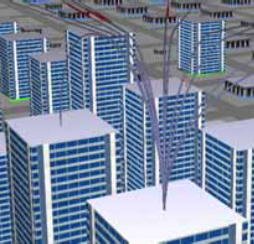
\includegraphics[scale=0.75]{Imagens/evospaces.png}
  	\textsf{\caption[EvoSpaces.]{EvoSpaces \cite{Alam2007}.\label{fig:evospaces}}}
\end{figure}

O EvoSpaces \cite{Alam2007}, mostrado na Figura \ref{fig:evospaces}, é uma ferramenta que provê a visualização da arquitetura e métricas de sistemas de software complexos em um mundo virtual 3D, utilizando metáforas familiares para ajudar no entendimento desse software. Aproveita o fato de que os sistemas são, muitas vezes, estruturados hierarquicamente para sugerir o uso de uma metáfora de cidades. As entidades, junto com suas relações, são representadas como glifos residenciais (casa, apartamento, escritório, etc), ao passo que as métricas dessas entidades são exibidas como posições e escalas visuais (tamanho, cor, etc). A ferramenta possui diferentes modos de interação, como \textit{zoom} e outras formas de navegação no ambiente virtual.

\begin{figure}[htb]
	\centering
  	\frame{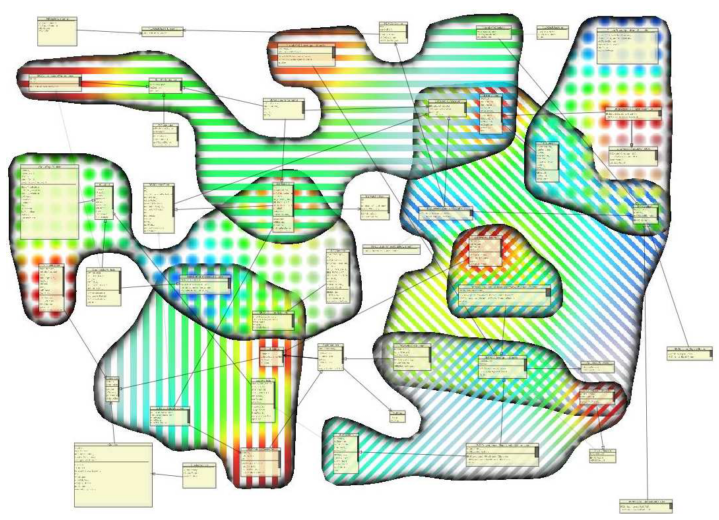
\includegraphics[scale=0.30]{Imagens/areas_of_interest.png}}
  	\textsf{\caption[Areas of Interest.]{Areas of Interest \cite{Byelas2009}.\label{fig:areas-of-interest}}}
\end{figure}

O Areas of Interest \cite{Byelas2009}, mostrado na Figura \ref{fig:areas-of-interest}, é uma técnica que consiste em aplicar um algoritmo que agrupa entidades de software com propriedades comuns, as engloba com um contorno e adiciona cores para descrever métricas de software. Para distinguir áreas de sobreposição, cada área tem uma textura diferente, como linhas horizontais, verticais, diagonais e círculos. Além disso, técnicas de sombreamento e transparência são usadas para melhorar a distinção entre várias áreas.

\subsection{Visualização da Evolução da Arquitetura de Software} \label{subsec:visualizacao-evolucao-arquitetura-software}

A evolução de um software tem sido destacada como um dos tópicos mais importantes na engenharia de software \cite{Novais2013}. Trata-se de uma tarefa complexa por ter que lidar com uma grande quantidade de dados: estima-se que 60\% do esforço na etapa de manutenção é para entender o software \cite{Corbi1989}. A visualização de software visa ajudar os \textit{stakeholders} a melhorar a compreensão do software, no entanto, elaborar metáforas visuais que representem efetivamente a dimensão tempo com todas as informações relacionadas a evolução do software é uma tarefa difícil \cite{Magnavita2015}.

No contexto da visualização da evolução da arquitetura de um software, um dos grandes desafios, além da quantidade de dados provenientes da evolução, é o crescente tamanho e complexidade do software. Apesar da dificuldade, é importante prover visualizações gerais da arquitetura, dos relacionamentos entre os módulos e das métricas, para cada versão \cite{Khan2012}.

\begin{figure}[htb]
	\centering
  	\frame{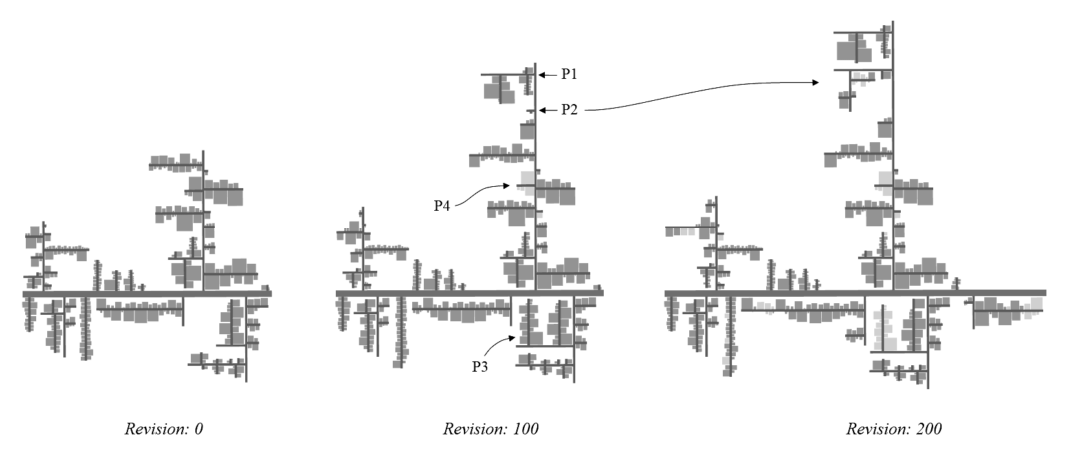
\includegraphics[scale=0.40]{Imagens/crococosmos.png}}
  	\textsf{\caption[CrocoCosmos.]{CrocoCosmos \cite{Steinbruckner2010b}.\label{fig:crococosmos}}}
\end{figure}

O \textit{CrocoCosmos} \cite{Steinbruckner2010b} é um exemplo de ferramenta que utiliza uma metáfora de cidades para representar a evolução estrutural da arquitetura de um software, onde ruas representam pacotes e construções refletem as classes Java. A sequência de representações visuais objetiva destacar as mudanças básicas na estrutura do software, como elementos que foram adicionados, removidos ou movidos dentro da hierarquia. A Figura \ref{fig:crococosmos} mostra um exemplo dessa ferramenta. O \textit{Code Flows} \cite{Telea2008} e o \textit{Successive Inheritance Graphs} \cite{Collberg2003} são outros exemplos de visualizações de evolução estrutural de arquitetura de software.

Outra forma de se exibir a evolução de um software é através das suas métricas. Elas encapsulam, sumarizam e proveem informações de qualidade sobre o código-fonte \cite{Langelier2008}. As métricas são essenciais para o entendimento contínuo e para a análise da qualidade do sistema durante todas as fases do seu ciclo de vida \cite{Khan2012}.

O \textit{CodeCity} \cite{Wettel2007} é uma visualização interativa em 3D que avalia a evolução estrutural de sistemas de software e as apresenta utilizando uma metáfora de cidades. As métricas são exibidas através de propriedades visuais dos artefatos da cidade: as propriedades das classes, como o número de métodos e de atributos, são mapeadas como a altura e o tamanho da base das construções, respectivamente; a profundidade dos pacotes é representada através da saturação de cores dos distritos. A Figura \ref{fig:codecity} exemplifica essa ferramenta.

\begin{figure}[htb]
	\centering
  	\frame{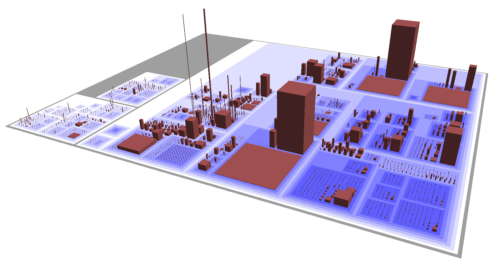
\includegraphics[scale=0.75]{Imagens/codecity.png}}
  	\textsf{\caption[CodeCity.]{Codecity \cite{Wettel2007}.\label{fig:codecity}}}
\end{figure}

Outras soluções que apresentam visualizações da evolução da arquitetura de um software através das métricas são: \textit{The Evolution Matrix} \cite{Lanza2001}, \textit{VERSO} \cite{Langelier2008}, \textit{RelVis} \cite{Pinzger2005} e \textit{SourceMiner Evolution} \cite{Novais2013a}.

\subsection{Estudos Empíricos em Visualização de Software} \label{subsec:estudos-empiricos-visualizacao-software}

As visualizações são importantes para ajudar na compreensão de vários aspectos de um software, além de ajudar a aumentar a produtividade do processo de desenvolvimento, lançando mão de metáforas visuais para representar esses aspectos. Entretanto, não significa que toda visualização de software é útil. Para cada técnica em particular, e para cada intenção de uso, é necessário avaliar a sua utilidade \cite{Diehl2007}. O objetivo principal de uma visualização é transmitir informações de forma compreensível, eficaz e fácil de lembrar. \citeauthor{Diehl2007} agrupa as avaliações das visualizações em dois grupos: quantitativa e qualitativa.

Os métodos quantitativos de avaliação medem propriedades da visualização ou propriedades do usuário interagindo com a visualização. Esse tipo de avaliação requer uma análise estatística dos resultados de um experimento controlado \cite{Diehl2007}.

Já o método qualitativo coleta dados sobre a experiência dos usuários com as visualizações, verbalizados em formato de relatórios. Os métodos qualitativos são de extrema importância quando se trata da percepção humana e da interação com uma visualização \cite{McConathy1993}, incluindo o fato de eles exigirem menos pessoas para o teste e cobrirem mais aspectos da visualização avaliada.

\citeauthor{komlodi2004information}, em sua pesquisa com cerca de 50 estudos de usuários de sistemas de visualização de informação, encontrou quatro áreas de avaliação:
\begin{enumerate}[(i)]
	\item \textit{Experimentos controlados comparando elementos de design}: esses estudos podem comparar elementos específicos;
	\item \textit{Avaliação de usabilidade de uma ferramenta}: esses estudos podem fornecer \textit{feedback} sobre problemas encontrados pelos usuários com uma ferramenta e mostrar como os \textit{designers} podem refinar o \textit{design};
	\item \textit{Experimentos controlados comparando duas ou mais ferramentas}: geralmente tentam comparar novas abordagens com o estado da arte;
	\item \textit{Estudos de caso de ferramentas em contextos realistas}: a vantagem dos estudos de caso é que eles relatam os usuários em seu ambiente natural fazendo tarefas reais, demonstrando viabilidade e utilidade no contexto. A desvantagem é que eles são demorados para conduzir e os resultados podem não ser replicáveis e generalizáveis.
\end{enumerate}

\citeauthor{Seriai2014} realizou um estudo de mapeamento sistemático de métodos de validação em visualização de software. Os autores definiram seis propriedades de classificação desses métodos:
\begin{enumerate}[(i)]
	\item \textit{Tipo de Investigação}: determina qual o tipo de estudo empírico foi usado: experimento, estudo de caso ou questionário;
	\item \textit{Tarefas}: especifica a natureza das tarefas envolvidas na avaliação. Elas são específicas quando o participante tem que resolver um problema específico, ou exploratórias quando o participante não tem uma tarefa específica para executar;
	\item \textit{Fonte de Dados}: caracteriza a fonte dos dados da visualização: industrial, \textit{open source} e/ou dados domésticos;
	\item \textit{Participantes}: determina o perfil dos participantes usados na avaliação, se houver: estudantes, profissionais ou ambos;
	\item \textit{Medidas}: especifica se a avaliação incluiu medidas objetivas, ou seja, sem ser baseadas no julgamento dos participantes. Caso contrário, as medidas poderiam ser subjetivas ou sem medida
	\item \textit{Referência de Comparação}: define se a ferramenta foi comparada a outras ferramentas.
\end{enumerate}

Como resultados, os autores destacam que 78,16\% dos artigos analisados utilizaram o método de estudo de caso, sendo destes, 65\% puramente análise qualitativa. Além disso, 72,5\% envolviam tarefas específicas na avaliação, 77\% dos artigos usaram ferramentas \textit{open source}, 70,1\% das avaliações foram realizadas sem participantes. Com relação às medidas, 60,9\% dos trabalhos coletaram medidas objetivas. Por fim, 77\% dos artigos não incluíram nenhuma comparação com outras abordagens. Baseado nesses resultados, os autores concluíram que a análise dos tipos de experimentos feitos mostra uma tendência em relação aos estudos de caso, tarefas específicas, fonte de dados \textit{open source}, sem participantes, com medidas objetivas e sem referência de comparação \cite{Seriai2014}.

\section{Ferramentas de Análise de Desempenho} \label{sec:ferramentas-analise-desempenho}

O tamanho e a complexidade das aplicações modernas aumentaram a demanda por ferramentas que coletem dados sobre o comportamento dinâmico dos programas, e portanto permitam aos desenvolvedores identificarem gargalos de desempenho nas suas aplicações com um mínimo de esforço. O processo de coleta automática e apresentação dos dados de desempenho de sistemas em execução é chamado de \textit{profiling} \cite{Dmitriev2004}.

Nesse contexto, o \textit{profiling} de \abrv[CPU -- \textit{Central Processing Unit}]{CPU}determina quanto tempo o programa gastou executando várias partes do código. Com isso, pode-se calcular o desempenho, em termos de tempo de execução, de determinada funcionalidade ou rotina. Já o \textit{profiling} de memória determina o número, tipos e ciclos de vida dos objetos que o programa aloca \cite{Dmitriev2004}. Existem outras modalidades, no entanto a de CPU e memória são as mais usadas.

Das diferentes técnicas de se realizar o \textit{profiling}, a baseada em instrumentação é a mais comum. Essa técnica trabalha inserindo, ou injetando, trechos especiais de código, chamados de código de instrumentação, na aplicação. A execução desses trechos gera eventos, como entrada/saída de métodos ou alocação de objetos. Esses dados são coletados, processados e, eventualmente, apresentados ao usuário. Com relação ao \textit{profiling} de CPU, essa técnica grava exatamente o número exato de eventos, ao invés de uma aproximação estatística (como acontece com o \textit{profiling} baseado em amostragem) \cite{Dmitriev2004}.

Uma das formas de utilizar o \textit{profiling} baseado em instrumentação é lançando mão do paradigma de programação orientado a aspectos, que permite o aumento da modularidade de um sistema através da separação de interesses. O princípio é que alguma lógica ou funcionalidade possa agir transversalmente entre as diferentes lógicas encapsuladas no sistema usando diferentes tipos de abstrações \cite{Bateman2009}. Para a linguagem de programação Java, o suporte a programação orientada a aspectos é feito usando a biblioteca \textit{AspectJ}.

Existem no mercado várias ferramentas que realizam a medição do atributo de qualidade de desempenho para a linguagem Java. Algumas delas são:
\begin{itemize}
	\item \textit{VisualVM} \cite{Vis}: distribuída gratuitamente com o \textit{Java Development Kit} (JDK), exibe o tempo de execução de cada método em tempo real e o usuário pode, à medida que deseja, tirar fotografias instantâneas da execução do software, os chamados \textit{snapshots};
	\item \textit{JProfiler} \cite{JProfiler}: ferramenta paga, pode exibir o \textit{call graph} de chamadas dos métodos em tempo real, com seus respectivos tempos de execução. Assim como o \textit{VisualVM}, a ferramenta oferece a possibilidade de guardar \textit{snapshots} de determinados momentos da execução;
	\item \textit{YoutKit Java Profiler} \cite{Profiler2016}: ferramenta paga que possui funcionalidades semelhantes às do \textit{JProfiler}.
\end{itemize}

Além das ferramentas de \textit{profiling}, outra maneira de se realizar a análise de desempenho de aplicações é utilizando ferramentas de gerenciamento de desempenho de aplicações, as chamadas APM. Essas ferramentas integram abordagens de mineração de dados de desempenho em ferramentas de monitoramento de desempenho disponíveis no mercado e são frequentemente utilizadas para detectar anomalias no desempenho \cite{Ahmed2016}. Exemplos desse tipo de ferramentas são o \textit{New Relic} \cite{Relic2016}, \textit{AppDynamics} \cite{Appdynamics}, \textit{Dynatrace} \cite{Dynatrace2016} e \textit{Pinpoint} \cite{Pinpoint2016}.

\section{\perfMinerName} \label{sec:perfminer}

A ferramenta \textit{\toolName} foi desenvolvida como uma extensão da ferramenta \textit{\perfMinerName}, a qual provê a avaliação de cenários de execução do sistema no que diz respeito a desvios de desempenho, de forma a minimizar a erosão de tal atributo de qualidade \cite{Pinto2015}.

A principal funcionalidade do \textit{\perfMinerName} é realizar a análise de desvio de desempenho entre duas versões de um sistema, revelando de maneira automatizada, as potenciais causas para o desvio nos cenários. Para isso, técnicas de análise dinâmica e mineração de repositório são usadas para estabelecer uma abordagem baseada em cenários para a avaliação do atributo de qualidade de desempenho, medido em termos de tempos de execução \cite{Pinto2015}.

Para atingir o objetivo de realizar a análise de desvio de desempenho, o \textit{\perfMinerName} define três fases, descritas nas subseções a seguir: (i) análise dinâmica; (ii) análise de desvio; e (iii) mineração de repositório.

\subsection{Fase 1: Análise Dinâmica} \label{subsec:fase1}

A fase de análise dinâmica consiste em realizar a execução dos cenários através de uma suíte de testes automatizados. Como resultado, essa fase gera um modelo de análise dinâmica, que é persistido em um banco de dados e contém informações sobre os \textit{traces} de execução do sistema, modelados por um grafo de chamadas dinâmico que representa cada execução dos cenários selecionados para determinada versão \cite{Pinto2015}. A Figura \ref{fig:perfminer-fase1} ilustra esta fase.

\begin{figure}[!htb]
   \centering
   \frame{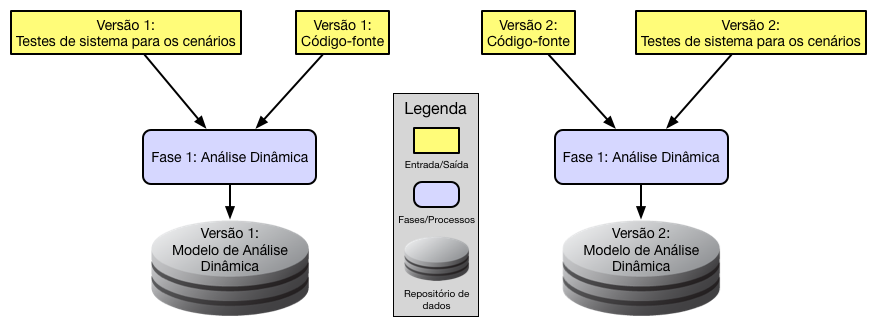
\includegraphics[scale=0.52]{Imagens/perfminer_fase_1.png}}
   \textsf{\caption[Fase 1 do \perfMinerName.]{Fase 1 do \perfMinerName.\label{fig:perfminer-fase1}}}
\end{figure}

O grafo é montado interceptando os métodos de entrada de cada cenário e instrumentando suas execuções, calculando o tempo de execução de cada nó, bem como informações sobre se o cenário falhou ou não. Esse grafo pode ser interpretado como uma estrutura em árvore onde cada nó é a execução de um método, onde os métodos de entrada representam os nós raiz \cite{Pinto2015}.

Duas informações são importantes nesse processo:
\begin{enumerate}[(i)]
   \item É fundamental que cada versão do sistema analisado possua testes automatizados para que o sistema seja executado. Caso o sistema não tenha testes automatizados, uma estratégia alternativa é utilizar ferramentas de teste de desempenho, como o \textit{JMeter} \cite{ApacheJMeter2016}, para submeter requisições que exercitem os cenários em um sistema web;
   \item Cada teste de sistema executado é considerado um cenário. Dessa forma, cada cenário analisado é representado na ferramenta com o seguinte nome: \textit{``Entry point for SimpleClassName.testMethodName''}.
\end{enumerate}

A ferramenta usa \textit{AspectJ} para definir um aspecto que instrumenta as execuções dos cenários, interceptando os métodos de entrada para montar o grafo de chamadas e calcular os tempos de execução dos cenários e dos seus métodos \cite{Pinto2015}. Vale salientar que todo o processo dessa fase deve ser executado uma vez para cada versão do sistema a ser analisado. Dessa forma, serão gerados dois modelos de análise dinâmica que são utilizados para calcular os desvios de desempenho dos cenários e métodos na fase seguinte.

A análise dinâmica é executada no mesmo computador para todas as versões, sob as mesmas condições. A suíte de testes para cada versão é executada 10 vezes. Essa quantidade de execuções ajuda a ter medições de desempenho mais precisas em termos de tempo de execução.

\subsection{Fase 2: Análise de Desvio} \label{subsec:fase2}

A segunda fase é a análise de desvio, que consiste em realizar a comparação do modelo de análise dinâmica, extraído durante a fase 1 (análise dinâmica) para cada uma das duas versões do sistema. Essa comparação revela os cenários e métodos que foram degradados ou otimizados durante a evolução. O artefato de saída desta fase é um relatório contendo os cenários e métodos degradados ou otimizados em termos de tempo de execução \cite{Pinto2015}. Esta fase pode ser vista na Figura \ref{fig:perfminer-fase2} adiante.

\begin{figure}[!htb]
   \centering
   \frame{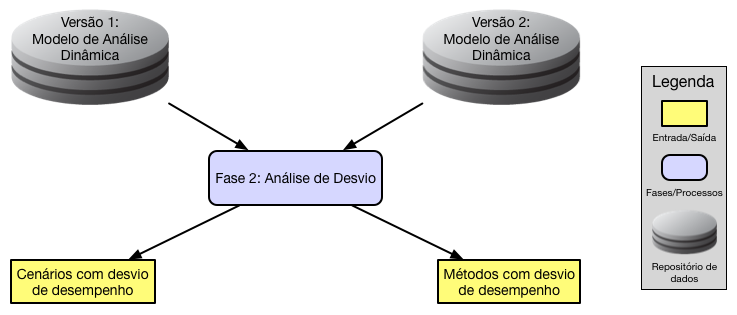
\includegraphics[scale=0.60]{Imagens/perfminer_fase_2.png}}
   \textsf{\caption[Fase 2 do \perfMinerName.]{Fase 2 do \perfMinerName.\label{fig:perfminer-fase2}}}
\end{figure}

Para realizar a comparação entre os tempos de execução, o \textit{\perfMinerName} pode utilizar duas estratégias: média aritmética e teste estatístico. A primeira compara a média do tempo de execução para cada método em ambas as versões. Se o valor da versão mais nova aumentou ou diminuiu mais do que um limiar configurado, é considerado que o método teve um desvio de desempenho. Já a segunda, usa um teste estatístico para observar se duas amostras independentes têm a mesma tendência. Neste caso, as amostras são formadas pelo conjunto dos valores dos tempos de execução para cada método comum em cada cenário \cite{Pinto2015}.

A estratégia de teste estatístico utilizado pela ferramenta é o Mann-Whitney U-Test \cite{Neuhauser2011}. Para esse teste, a ferramenta usa um valor padrão para o nível de significância (\textit{alpha}) de 0,05. Dado um método, se o \textit{p-value} calculado for igual ou menor do que o nível de significância, houve um desvio de desempenho para este método. Para os casos em que há o desvio, o tempo médio de execução é usado para determinar se houve uma degradação ou otimização. Embora, no geral, os desenvolvedores e arquitetos estejam interessados em degradações, a ferramenta também sinaliza as otimizações. Isso pode se tornar interessante, pois os desenvolvedores podem checar se algumas modificações esperadas realmente diminuíram o tempo de execução \cite{Pinto2015}.

\subsection{Fase 3: Mineração de Repositório} \label{subsec:fase3}

A última fase realiza a mineração nos repositórios de controle de versões e gerenciador de tarefas com o intuito de encontrar os \textit{commits} e tarefas que alteraram os métodos identificados na fase anterior. Para cada método detectado com desvio de desempenho (degradação ou otimização), esta fase recupera os \textit{commits} do sistema de controle de versões. Se esse \textit{commit} alterou linhas dentro do método detectado, o número da respectiva tarefa é procurado na mensagem de \textit{commit}. O número da tarefa é usado para procurá-la no sistema de gerenciamento de tarefas em busca de informações extras, tais como o tipo da tarefa (defeito, melhoria, nova funcionalidade, etc) \cite{Pinto2015}. A Figura \ref{fig:perfminer-fase3} ilustra essa fase.

\begin{figure}[!htb]
   \centering
   \frame{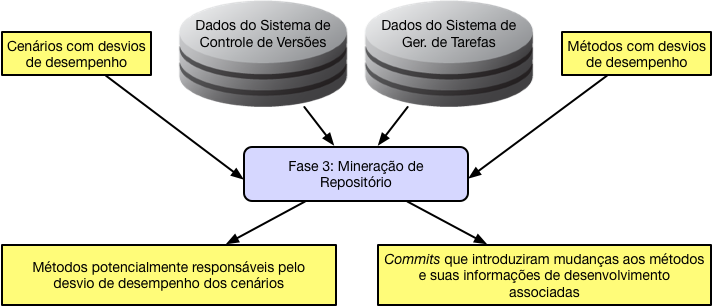
\includegraphics[scale=0.62]{Imagens/perfminer_fase_3.png}}
   \textsf{\caption[Fase 3 do \perfMinerName.]{Fase 3 do \perfMinerName.\label{fig:perfminer-fase3}}}
\end{figure}

É importante notar que os métodos identificados com desvios de desempenho nas fases anteriores, mas que não foram alterados durante a evolução, são também selecionados e armazenados, contudo, não estarão presentes no relatório final por, provavelmente, não representar causas reais do desvio de desempenho do cenário. Eles podem ter sido impactados por outros métodos na hierarquia de chamadas \cite{Pinto2015}.

A abordagem completa do \textit{\perfMinerName} pode ser vista na Figura \ref{fig:perfminer-completo} adiante. Os artefatos de saída são usados como entradas para as fases seguintes, até a geração do relatório final. Os testes de sistemas em ambas as versões são considerados como os cenários para a análise e apenas os cenários e métodos comuns entre as versões são comparados.

\begin{figure}[!htb]
   \centering
   \frame{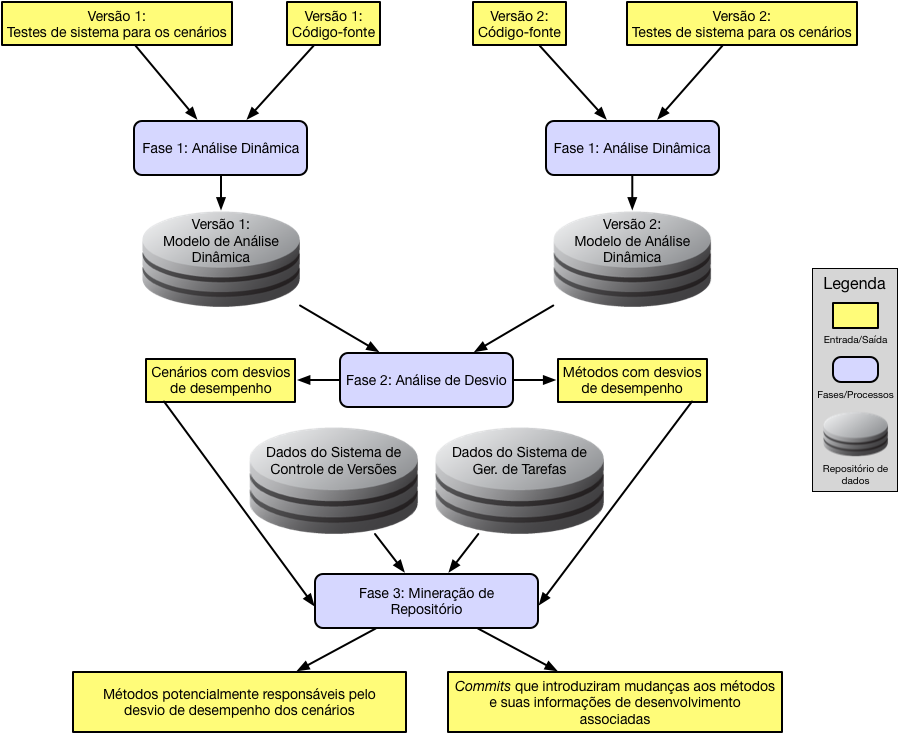
\includegraphics[scale=0.50]{Imagens/perfminer_completo.png}}
   \textsf{\caption[Abordagem completa do \perfMinerName.]{Abordagem completa do \perfMinerName.\label{fig:perfminer-completo}}}
\end{figure}

\section{Considerações} \label{sec:consideracoes-cap2}

Os conceitos apresentados neste capítulo são importantes para o entendimento da proposta. Com relação ao conceito de arquitetura de software, a ferramenta \textit{\perfMinerName}, utilizada neste trabalho, é focada principalmente na implementação do sistema, e não nos componentes arquiteturais ou relacionamentos entre eles. Além disso, apesar de existirem vários atributos de qualidade, apenas o de desempenho, medido em termos de tempo de execução, é considerado. Com relação aos cenários, é a forma com a qual a avaliação da arquitetura do software é guiada e eles são definidos, no contexto deste trabalho, como sendo um caso de teste automatizado do sistema.

A respeito da visualização de software, a ferramenta proposta utiliza representações visuais para exibir aspectos dinâmicos e a evolução do atributo de qualidade de desempenho ao longo das versões do sistema. Assim, como o \textit{\perfMinerName} não trata dos componentes arquiteturais ou dos seus relacionamentos, não são usadas representações visuais para tal fim na ferramenta proposta.

Foram mencionadas neste capítulo ferramentas de análise de desempenho, como as de \textit{profiling} e APM, pois é possível medir o desempenho de aplicações utilizando-as. Entretanto, a ferramenta \textit{\toolName} se diferencia pela identificação automatizada da evolução do desempenho e a sua apresentação através de metáforas visuais. Com relação a técnica de coleta automática de dados, o \textit{\perfMinerName} utiliza a instrumentação de código através do \textit{AspectJ}.
	
	% Capitulo 3: Terceiro capítulo (arquivo Includes/Capitulo3.tex)
	% Capíulo 3
\chapter{\toolName} \label{ch:visualizacoes}

{\color{red}rever texto a seguir...}

{\color{red}para cada visualização, comentar quais seriam os benefícios e o que os desenvolvedores podem tirar de informações delas...}

Este capítulo apresenta o conjunto de visualizações proposto como extensão à ferramenta \textit{\perfMinerName}. A seção \ref{sec:perfminer} destaca o funcionamento dessa ferramenta. A seção \ref{visao-geral-architecture-qa-evolution} mostra uma visão geral sobre o funcionamento das visualizações propostas. As seções \ref{sec:visualizacao1}, \ref{sec:visualizacao2} e \ref{sec:visualizacao3} descrevem cada uma das visualizações, sendo esta última em detalhes, com suas características, propriedades visuais, funcionamento e exemplo de uso. Por fim, são reportadas considerações finais sobre o capítulo na seção \ref{sec:consideracoes-cap3}.

\section{\perfMinerName} \label{sec:perfminer}

A implementação das visualizações está sendo desenvolvida como uma extensão da ferramenta \textit{\perfMinerName}, a qual provê a avaliação contínua de cenários no que diz respeito a análise de desvios de desempenho, de forma a minimizar a erosão de atributos de qualidade em cenários arquiteturalmente relevantes \cite{Pinto2015}.

A principal funcionalidade do \textit{\perfMinerName} é realizar a análise de desvio de desempenho entre duas versões de um sistema, revelando de maneira automatizada, as potenciais causas para o desvio nos cenários. Para isso, técnicas de análise dinâmica e mineração de repositório são usadas para estabelecer uma abordagem baseada em cenários para a avaliação do atributo de qualidade de desempenho, medido em termos de tempos de execução \cite{Pinto2015}.

\subsection{Funcionamento} \label{subsec:funcionamento-perfminer}

Para atingir o objetivo de realizar a análise de desvio de desempenho, foram definidas três fases, descritas com maiores detalhes nas subseções a seguir: (i) análise dinâmica; (ii) análise de desvio; e (iii) mineração de repositório.

\subsubsection{Fase 1: Análise Dinâmica} \label{subsec:fase1}

A fase de análise dinâmica consiste em realizar a execução dos cenários através de uma suíte de testes automatizados. Como resultado, essa fase gera um modelo de análise dinâmica, que é persistido em um banco de dados e contém informações sobre os \textit{traces} de execução do sistema, modelados por um grafo de chamadas dinâmico que representa cada execução dos cenários selecionados para determinada versão \cite{Pinto2015}. A figura \ref{fig:perfminer-fase1} a seguir ilustra esta fase.

\begin{figure}[!htb]
   \centering
   \frame{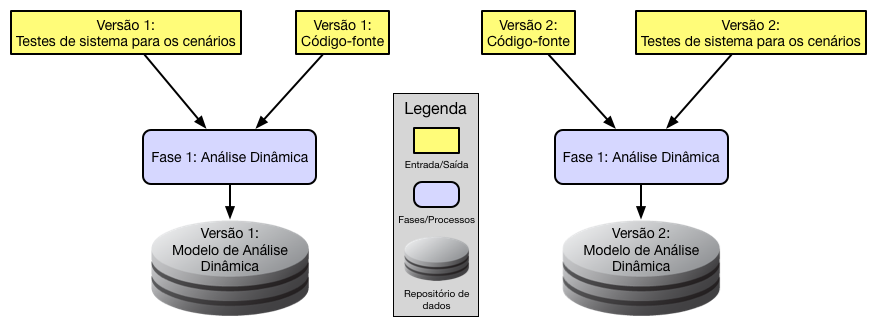
\includegraphics[scale=0.52]{Imagens/perfminer_fase_1.png}}
   \textsf{\caption[Fase 1 do \perfMinerName.]{Fase 1 do \perfMinerName.\label{fig:perfminer-fase1}}}
\end{figure}

O grafo é montado interceptando os métodos de entrada de cada cenário e instrumentando suas execuções, calculando o tempo de execução de cada nó, bem como informações sobre se o cenário falhou ou não. Esse grafo pode ser interpretado como uma estrutura em árvore onde cada nó é a execução de um método, onde os métodos de entrada representam os nós raiz \cite{Pinto2015}.

Duas informações são importantes nesse processo:
\begin{enumerate}[(i)]
   \item É fundamental que cada versão do sistema analisado possua testes automatizados para que o sistema seja executado. Caso o sistema não tenha testes automatizados, uma estratégia alternativa é utilizar ferramentas de teste de desempenho, como o \textit{JMeter} \cite{ApacheJMeter2016}, para submeter requisições que exercitem os cenários em um sistema web;
   \item Cada teste de sistema executado é considerado um cenário. Dessa forma, cada cenário analisado é representado na ferramenta com o seguinte nome: \textit{``Entry point for SimpleClassName.testMethodName''}.
\end{enumerate}

A ferramenta usa \textit{AspectJ} para definir um aspecto que instrumenta as execuções dos cenários, interceptando os métodos de entrada para montar o grafo de chamadas e calcular os tempos de execução dos cenários e dos seus métodos \cite{Pinto2015}.

De maneira sumária, o processo da figura \ref{fig:perfminer-fase1} se inicia com a execução dos testes de sistema, que são, então, interceptados pelo \textit{AspectJ} a fim de calcular seus tempos de execução. Após isso, o modelo de análise dinâmica resultante é persistido no banco de dados. Vale salientar que todo o processo dessa fase deve ser executado uma vez para cada versão do sistema a ser analisado. Dessa forma, serão gerados dois modelos de análise dinâmica que são utilizados para calcular os desvios de desempenho dos cenários e métodos na fase seguinte.

A análise dinâmica é executada no mesmo computador para todas as versões, nas mesmas condições e com todos os serviços não essenciais desabilitados (por exemplo: atualizações, antivírus, memória virtual). A suíte de testes para cada versão é executada, no mínimo, 10 vezes. Essa quantidade de execuções ajuda a ter medições de desempenho mais precisas em termos de tempo de execução.

\subsubsection{Fase 2: Análise de Desvio} \label{subsec:fase2}

A segunda fase é a análise de desvio, que consiste em realizar a comparação do modelo de análise dinâmica, extraído durante a fase de análise dinâmica, para cada uma das duas versões do sistema. Essa comparação revela os cenários e métodos que foram degradados ou otimizados durante a evolução. O artefato de saída desta fase é um relatório contendo os cenários e métodos degradados ou otimizados em termos de tempo de execução \cite{Pinto2015}. Esta fase pode ser vista na figura \ref{fig:perfminer-fase2} adiante.

\begin{figure}[!htb]
   \centering
   \frame{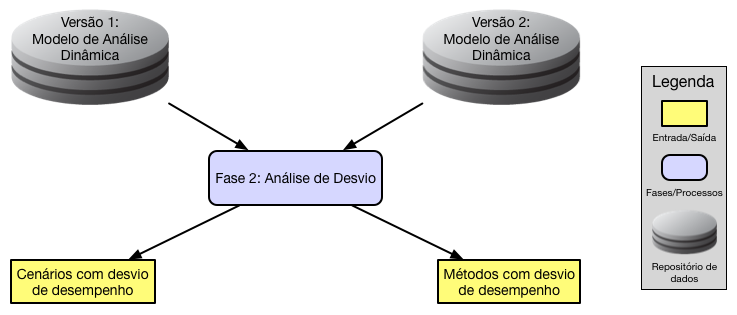
\includegraphics[scale=0.60]{Imagens/perfminer_fase_2.png}}
   \textsf{\caption[Fase 2 do \perfMinerName.]{Fase 2 do \perfMinerName.\label{fig:perfminer-fase2}}}
\end{figure}

Para realizar a comparação entre os tempos de execução, o \textit{\perfMinerName} pode utilizar duas estratégias: média aritmética e teste estatístico. A primeira compara a média do tempo de execução para cada método em ambas as versões. Se o valor da versão mais nova aumentou ou diminuiu mais do que um limiar configurado, é considerado que o método teve um desvio de desempenho. Já a segunda, usa um teste estatístico para observar se duas amostras independentes têm a mesma tendência. Neste caso, as amostras são formadas pelo conjunto dos valores dos tempos de execução para cada método comum em cada cenário \cite{Pinto2015}.

A estratégia de teste estatístico utilizado pela ferramenta é o Mann-Whitney U-Test \cite{Neuhauser2011}. Para esse teste, a ferramenta usa um valor padrão para o nível de significância (\textit{alpha}) de 0,05. Dado um método, se o \textit{p-value} calculado for igual ou menor do que o nível de significância, houve um desvio de desempenho para este método. Para os casos em que há o desvio, o tempo médio de execução é usado para determinar se houve uma degradação ou otimização. Embora, no geral, os desenvolvedores e arquitetos estejam interessados em degradações, a ferramenta também sinaliza as otimizações. Isso pode se tornar interessante, pois os desenvolvedores podem checar se algumas modificações esperadas realmente diminuíram o tempo de execução \cite{Pinto2015}.

\subsubsection{Fase 3: Mineração de Repositório} \label{subsec:fase3}

A última fase realiza a mineração nos repositórios de controle de versões e gerenciador de tarefas com o intuito de encontrar os \textit{commits} e tarefas que alteraram os métodos identificados na fase anterior. Para cada método detectado com desvio de desempenho (degradação ou otimização), esta fase recupera os commits do sistema de controle de versões. Se esse \textit{commit} alterou linhas dentro do método detectado, o número da respectiva tarefa é procurado na mensagem de \textit{commit}. O número da tarefa é usado para procurá-la no sistema de gerenciamento de tarefas em busca de informações extras, tais como o tipo da tarefa (defeito, melhoria, nova funcionalidade, etc) \cite{Pinto2015}. A figura \ref{fig:perfminer-fase3} ilustra essa fase.

\begin{figure}[!htb]
   \centering
   \frame{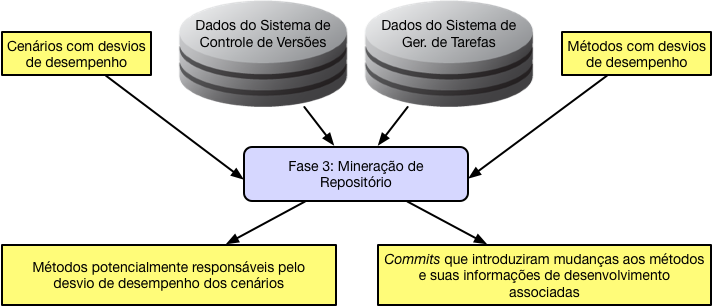
\includegraphics[scale=0.62]{Imagens/perfminer_fase_3.png}}
   \textsf{\caption[Fase 3 do \perfMinerName.]{Fase 3 do \perfMinerName.\label{fig:perfminer-fase3}}}
\end{figure}

É importante notar que os métodos identificados com desvios de desempenho nas fases anteriores, mas que não foram alterados durante a evolução, são também selecionados e armazenados, contudo, não estarão presentes no relatório final por, provavelmente, não representar causas reais do desvio de desempenho do cenário. Eles podem ter sido impactados por outros métodos na hierarquia de chamadas \cite{Pinto2015}.

A abordagem completa do \textit{\perfMinerName} pode ser vista na figura \ref{fig:perfminer-completo} adiante. Os artefatos de saída são usados como entradas para as fases seguintes, até a geração do relatório final. Os testes de sistemas em ambas as versões são considerados como os cenários para a análise e apenas os cenários e métodos comuns entre as versões são comparados.

\begin{figure}[!htb]
   \centering
   \frame{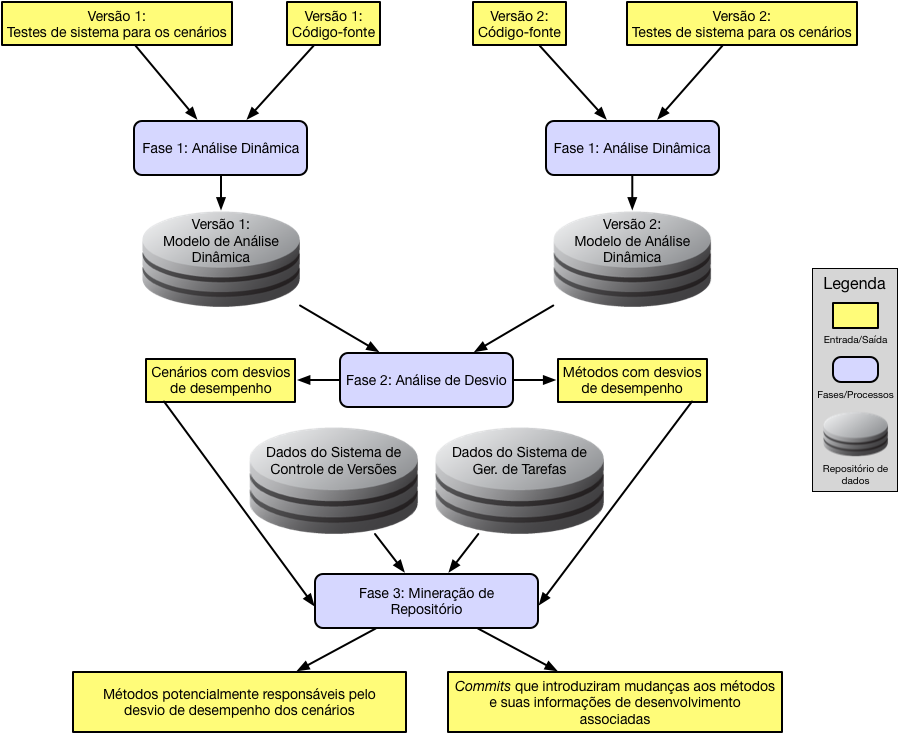
\includegraphics[scale=0.50]{Imagens/perfminer_completo.png}}
   \textsf{\caption[Abordagem completa do \perfMinerName.]{Abordagem completa do \perfMinerName.\label{fig:perfminer-completo}}}
\end{figure}

\begin{figure}[!htb]
   \centering
   \frame{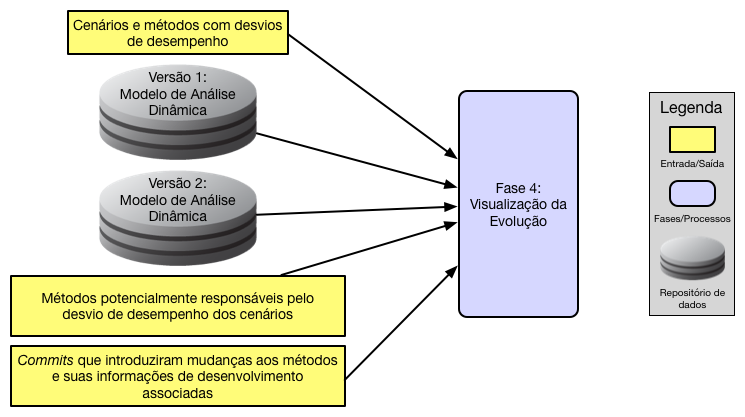
\includegraphics[scale=0.60]{Imagens/perfminer_fase_4.png}}
   \textsf{\caption[Fase 4 do \perfMinerName.]{Fase 4 do \perfMinerName.\label{fig:perfminer-fase4}}}
\end{figure}

As visualizações propostas como extensão da ferramenta utilizam os artefatos de saída gerados após a execução completa da abordagem, caracterizando assim mais uma fase da ferramenta: a Fase 4. Como ilustra a figura \ref{fig:perfminer-fase4} a seguir, os artefatos de saída utilizados pelas visualizações são: (i) os modelos de análise dinâmica de ambas as versões, (ii) os relatórios de cenários e métodos com desvios de desempenho, (iii) os métodos potencialmente responsáveis pelo desvio de desempenho dos cenários e (iv) os \textit{commits} que introduziram mudanças aos métodos, bem como suas informações de desenvolvimento associadas. Cada uma das visualizações implementadas utilizam total ou parcialmente os artefatos gerados nas fases anteriores, de acordo com o seu propósito.

\section{Visão Geral} \label{sec:visao-geral-architecture-qa-evolution}

A extensão ao \textit{\perfMinerName} foi implementada na forma de uma aplicação web, intitulada de \textit{Architecture QA Evolution}. O processamento do \textit{\perfMinerName} em suas fases 1, 2 e 3 não foi alterado, continuando \textit{standalone}. A escolha por esse tipo de aplicação se deu pelo fato de sua execução ocorrer em um ambiente distribuído, onde cada parte que compõe a aplicação está localizada em locais diferentes. Por exemplo, a interface com o usuário reside em sua estação de trabalho, ao passo que o servidor e o banco de dados estão localizados em outro computador.

Por ser web, os usuários da aplicação, como os desenvolvedores e arquitetos, podem utilizá-la sem a necessidade de instalar nenhum módulo nas suas estações de trabalho. Essa é uma importante característica da extensão à ferramenta, fazendo com que esta se diferencie das outras ferramentas mencionadas neste trabalho. A ideia é que distribuição e facilidade de acesso façam com que a equipe de desenvolvimento acompanhe mais adequadamente a evolução do atributo de qualidade de desempenho.

A implementação foi feita utilizando o \textit{framework} web Grails\footnote{https://grails.org}, banco de dados relacional PostgreSQL\footnote{https://www.postgresql.org} e o \textit{layout} das páginas foi elaborado lançando mão do \textit{framework front-end} Bootstrap\footnote{http://getbootstrap.com}. As visualizações foram geradas a partir de \textit{scripts} em JavaScript através da biblioteca JointJS\footnote{https://www.jointjs.com}. A estrutura das páginas web da ferramenta é dividida em três partes: canto superior, canto esquerdo e centro.

No canto superior situa-se uma barra de título, onde é apresentado o nome do sistema e o nome da página atual exibida. Na figura \ref{fig:pagina-inicial}, o nome do sistema é identificado como \texttt{\toolName} ao passo que o nome da página é \texttt{Analyzed Systems}.

Já no canto esquerdo é encontrada uma barra de menus contendo dois itens:
\begin{itemize}
   \item Nova análise (
\includegraphics[height=1.5em,valign=b]{Imagens/icon_new_analysis.png}): a partir deste item o usuário pode iniciar uma nova análise, que será descrita com maiores detalhes posteriormente;
   \item Sistemas analisados (
\includegraphics[height=1.5em,valign=b]{Imagens/icon_analyzed_systems.png}): é a página inicial mostrada na figura \ref{fig:pagina-inicial} explicada adiante.
\end{itemize}

Ao centro está a área principal da aplicação, onde são exibidas os conteúdos das páginas acessadas pelo usuário. Na página inicial exibida na figura \ref{fig:pagina-inicial}, pode ser verificada uma tabela contendo todos os sistemas analisados. Cada linha da tabela representa uma análise, onde são exibidas: a versão anterior (\textit{Version From}), versão posterior (\textit{Version To}), \textit{status} e ações (\textit{Actions}). No exemplo da figura, dois sistemas foram analisados pela ferramenta: o sistema \textit{System A} teve três análises e o sistema \textit{System B} teve quatro análises.

Dependendo do \textit{status} de cada análise, algumas ações pode ser tomadas. Caso o \textit{status} seja \texttt{COMPLETED}, o usuário pode navegar até a visualização de sumarização de cenários (
\includegraphics[height=1.5em,valign=b]{Imagens/visualizacao_1_icone.png}) ou apagar a análise (
\includegraphics[height=1.4em,valign=b]{Imagens/icon_delete_analysis.png}). Caso seja \texttt{ERROR}, a única ação que pode ser tomada é a de apagar a análise para que esta possa ser realizada novamente. Se o \textit{status} for \texttt{PENDING}, nenhuma ação pode ser efetuada uma vez que a análise ainda está em processamento.

\begin{figure}[htb]
   \centering
   \frame{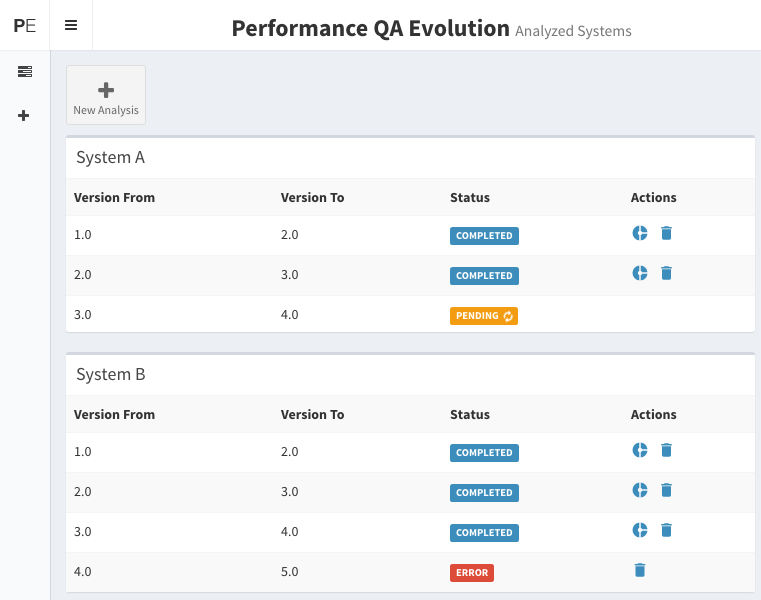
\includegraphics[scale=0.60]{Imagens/pagina_inicial.png}}
   \textsf{\caption[Página inicial da aplicação.]{Página inicial da aplicação.\label{fig:pagina-inicial}}}
\end{figure}

\subsection{Nova Análise} \label{subsec:new-analysis}

Para que o usuário da ferramenta obtenha acesso às visualizações é necessário que seja realizada uma análise dos artefatos gerados pelo \textit{\perfMinerName} onde, após o processamento, sejam gerados os dados responsáveis por supri-las.

A partir do menu de \texttt{Nova Análise} (
\includegraphics[height=1.5em,valign=b]{Imagens/icon_new_analysis.png}) ou do botão com o mesmo nome e ícone situado na página inicial (figura \ref{fig:pagina-inicial}), o usuário pode navegar até a página responsável por essa funcionalidade, exibida na figura \ref{fig:new-analysis}.

\begin{figure}[htb]
   \centering
   \frame{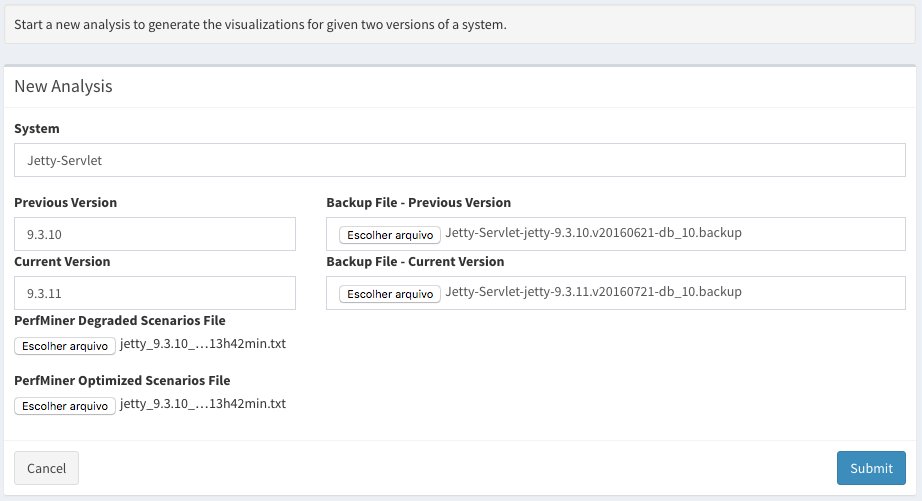
\includegraphics[scale=0.50]{Imagens/new_analysis.png}}
   \textsf{\caption[Página da funcionalidade de Nova Análise.]{Página da funcionalidade de Nova Análise.\label{fig:new-analysis}}}
\end{figure}

Nessa página, o usuário precisa informar os dados e arquivos necessários para que uma análise seja feita. No primeiro campo, o nome do sistema ao qual se deseja realizar a análise é informado. Após isso, é informada a versão anterior do sistema, no campo \texttt{Previous Version}, e o seu respectivo arquivo de \textit{backup} contendo os dados resultantes da análise do \textit{\perfMinerName}, no campo \texttt{Backup File - Previous Version}. Igualmente é feito para os campos \texttt{Current Version} e \texttt{Backup File - Current Version}, desta vez para a versão atual do sistema. Por fim, é necessário informar os arquivos contendo os cenários e métodos com desvio de desempenho, um para degradação de desempenho, no campo \texttt{\perfMinerName Degraded Scenarios File}, e outro para otimização de desempenho, no campo \texttt{\perfMinerName Optimized Scenarios File}.

\subsubsection{Funcionamento} \label{subsec:new-analysis-overview}

O funcionamento geral desta funcionalidade é ilustrado na figura \ref{fig:funcionamento-geral-nova-analise}. Vale salientar que esse processamento faz parte da fase 4 do \textit{\perfMinerName}, conforme exposto na figura \ref{fig:perfminer-fase4}. No primeiro passo desse processo (passo 1), o usuário realiza a requisição solicitando que uma nova análise seja realizada, de acordo com os parâmetros e arquivos informados na página da figura \ref{fig:new-analysis}.

\begin{figure}[!htb]
   \centering
   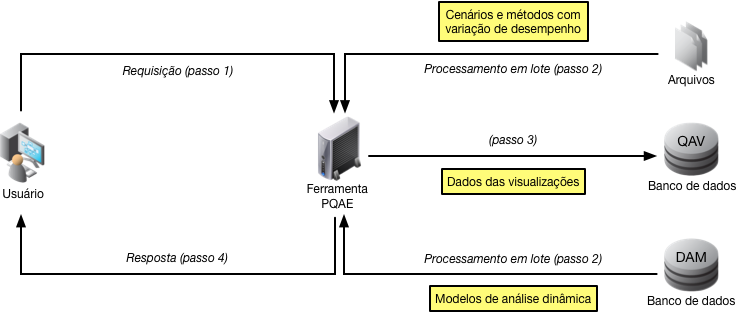
\includegraphics[scale=0.62]{Imagens/funcionamento_geral_nova_analise.png}
   \textsf{\caption[Funcionamento do processamento de uma nova análise.]{Funcionamento do processamento de uma nova análise.\label{fig:funcionamento-geral-nova-analise}}}
\end{figure}

Quando o servidor (Ferramenta PQAE) recebe essa requisição, inicia-se o processamento em lote (passo 2). Esse processamento recupera os arquivos contendo os cenários e métodos com desvio de desempenho que foram enviados pelo usuário, os arquivos de \textit{backups} referentes a versão anterior e atual a ser analisada. Os bancos de dados são restaurados e, então, os modelos de análise dinâmica para cada uma das versões são recuperadas desse banco de dados (identificado por \abrv[DAM -- \textit{Dynamic Analysis Model}]{DAM}– \textit{Dynamic Analysis Model}). De posse de todos esses dados, é realizado um processamento para determinar todos os dados que dão suporte às visualizações oferecidas pela ferramenta. Após isso, no passo 3, os dados resultantes são salvos em um banco de dados (identificado por \abrv[QAV -- \textit{Quality Attribute Visualization}]{QAV}– \textit{Quality Attribute Visualization}). Ao final, o usuário recebe a resposta de que o processamento requisitado foi efetuado com sucesso, no passo 4.

Detalhadamente, no processamento em lote, iniciado no passo 2, os arquivos de saída do \textit{\perfMinerName} contendo informações sobre os cenários e métodos com desvio de desempenho são lidos e os modelos de análise dinâmica de ambas as versões são recuperados do banco de dados DAM. A partir de então, os dados para cada visualização começam a ser processados. Os passos 2 e 3 da figura \ref{fig:funcionamento-geral-nova-analise} são detalhados no diagrama de atividades da figura \ref{fig:nova-analise-passos-2-3}.

De posse desses artefatos, os nós do grafo de chamadas são recuperados e a partir deles são determinados os métodos que foram adicionados ou removidos comparando os nós da versão atual com os da anterior. Depois disso, a partir dos métodos indicados pelos arquivos de saída do \textit{\perfMinerName}, são determinados os nós com desvios de desempenho, seja degradação ou otimização.

Na ferramenta, os nós identificados como adicionados, removidos e com desvio de desempenho são candidatos a serem exibidos. Optou-se por apresentar apenas os nós com desvio, nós adicionados, removidos e poucos nós sem desvio de desempenho, mas que ajudam a tornar o grafo legível, de modo que poucos nós são renderizados no navegador do usuário. Essa decisão levou em consideração a quantidade de nós de um cenário, que pode passar dos milhares, o desempenho da própria aplicação web e um possível ganho no entendimento da visualização do grafo de chamadas por parte do usuário.

\begin{figure}[!htb]
   \centering
   \frame{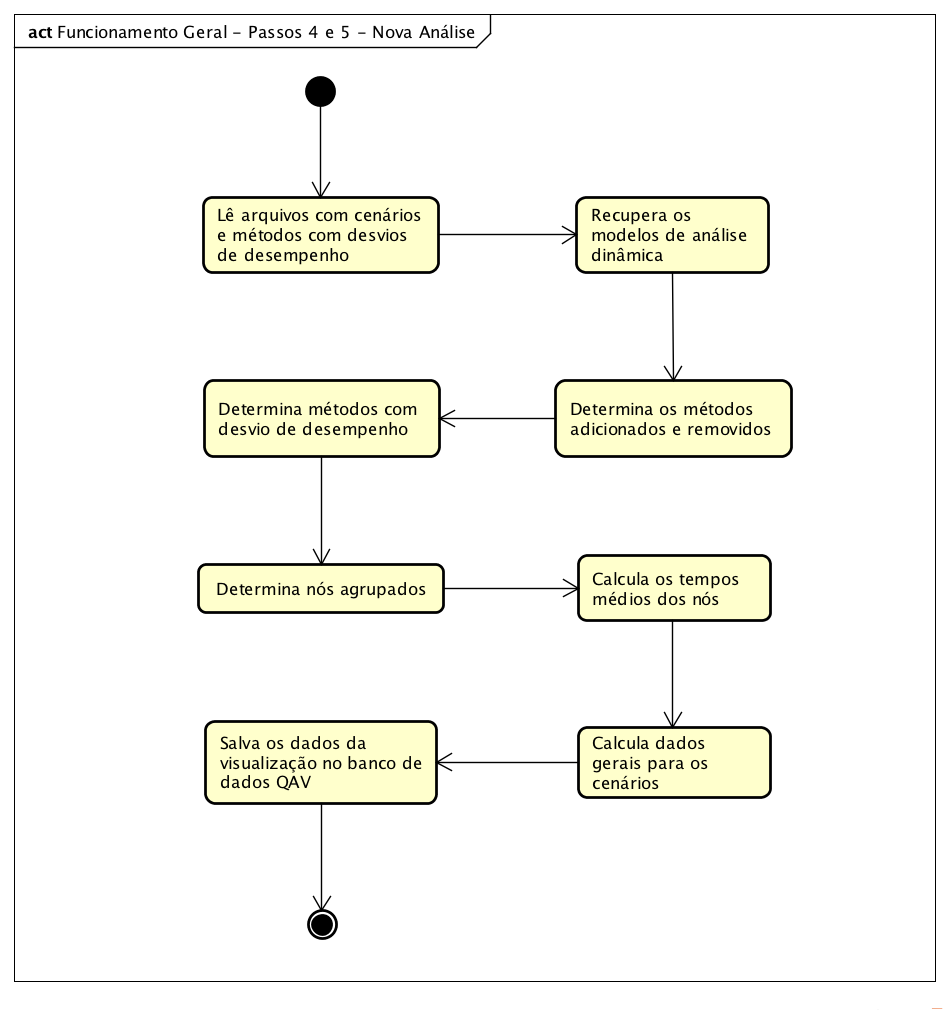
\includegraphics[scale=0.45]{Imagens/funcionamento_geral_nova_analise_diagrama_atividades.png}}
   \textsf{\caption[Passos 2 e 3 da realização de uma nova análise.]{Passos 2 e 3 da realização de uma nova análise.\label{fig:nova-analise-passos-2-3}}}
\end{figure}

Após determinar os nós com desvios de desempenho, são criados nós de agrupamento para representar os que não serão exibidos na visualização. Depois disso, os tempos médios dos nós a serem exibidos são calculados, levando em consideração todas as ocorrências do método no cenário.

Para a visualização da sumarização de cenários, os dados gerais de todos os cenários são calculados e, juntamente com os dados da visualização do grafo de chamadas calculados anteriormente, são salvos no banco de dados QAV no passo 3, marcando o fim do processo.

É importante frisar que o processamento em lote é executado apenas uma vez para duas versões de um sistema, sendo necessário para gerar os dados que possibilitam aos usuários um rápido tempo de resposta na requisição das visualizações.

\FloatBarrier

\subsubsection{Bancos de Dados} \label{subsec:databases}

Os bancos de dados DAM e QAV mencionados anteriormente têm funções distintas. O DAM é utilizado pelo \textit{\perfMinerName} para armazenar os dados coletados na análise dinâmica. Já o QAV é próprio da ferramenta \textit{\toolName} e armazena os dados que dão suporte às visualizações, funcionando também como um \textit{cache}, minimizando o tempo de resposta do servidor para o usuário.

\paragraph{DAM - \textit{Dynamic Analysis Model}} \label{par:estrutura-dados-dam}

O resultado do processamento da fase 1 do \textit{\perfMinerName} gera um modelo de análise dinâmica que contém informações sobre os \textit{traces} de execução do sistema, como mencionado na subseção \ref{subsec:fase1}. Esse modelo é persistido no banco de dados DAM, sendo usado, posteriormente, na extensão proposta por este trabalho para gerar as visualizações. A figura \ref{fig:perfminer-class-diagram} a seguir mostra o diagrama de classes parcial desse modelo.

\begin{figure}[!htb]
   \centering
   \frame{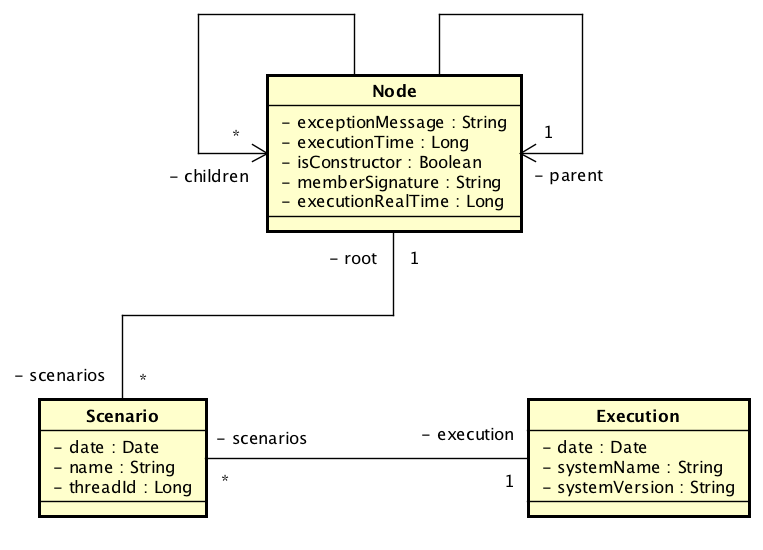
\includegraphics[scale=0.50]{Imagens/perf_miner_class_diagram.png}}
   \textsf{\caption[Diagrama de classes parcial do \textit{\perfMinerName}.]{Diagrama de classes parcial do \textit{\perfMinerName}.\label{fig:perfminer-class-diagram}}}
\end{figure}

A classe \texttt{Execution} representa uma execução específica do \textit{\perfMinerName} para um sistema. Possui atributos que indicam o nome do sistema, a versão e a data que a análise foi iniciada. Já a classe \texttt{Scenario} é o modelo para cada cenário executado. Os cenários têm um nome, uma data que indica quando foi analisado, o \texttt{id} da \textit{thread} que o executou, o contexto para representar requisições web (em caso de sistemas web) e o nó raiz.

A classe \texttt{Node} representa todo membro (método ou construtor) executado dentro de um cenário em particular. Essa classe possui atributos para indicar a assinatura do método ou construtor, uma mensagem se alguma exceção acontecer durante a execução, o tempo de execução total do membro, o tempo de execução do próprio membro, uma propriedade booleana que indica se o nó representa ou não um construtor e dois autorrelacionamentos: um para indicar o nó pai e outro para indicar os nós filhos. Uma atenção especial merece ser dada aos dois tempos de execução: a propriedade \texttt{executionRealTime} indica o tempo de execução do próprio método ou construtor, sem considerar os tempos de execução dos nós filhos. Já a propriedade \texttt{executionTime} representa o tempo total de execução do membro, considerando os tempos dos membros filhos.

\paragraph{QAV - \textit{Quality Attribute Visualization}} \label{par:estrutura-dados-qav}

A ferramenta faz uso de outro banco de dados além do DAM: o QAV. Essa base de dados é responsável por armazenar os dados que darão suporte às visualizações. A figura \ref{fig:archvis-class-diagram} a seguir mostra o diagrama de classes para esse modelo.

\begin{figure}[!htb]
   \centering
   \frame{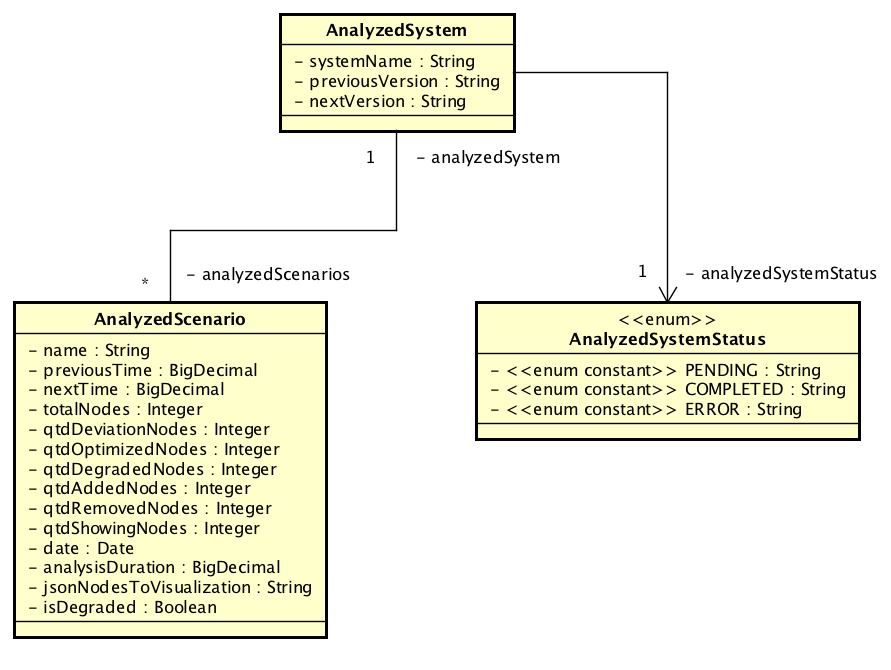
\includegraphics[scale=0.50]{Imagens/arch_vis_class_diagram.png}}
   \textsf{\caption[Diagrama de classes da extensão proposta.]{Diagrama de classes da extensão proposta.\label{fig:archvis-class-diagram}}}
\end{figure}

A classe \texttt{AnalyzedSystem} representa uma análise para dado sistema, em determinadas versões. Possui propriedades para o nome do sistema, versão anterior e versão posterior. Cada análise possui um \textit{status}, definido pela propriedade \texttt{analyzedSystemStatus} dessa classe, do tipo \texttt{AnalyzedSystemStatus}. Essa propriedade pode assumir um dos três valores a seguir: \texttt{PENDING} (análise em andamento), \texttt{COMPETED} (análise finalizada), \texttt{ERROR} (análise com erro - necessário novo processamento).

A classe \texttt{AnalyzedScenario} reflete cada cenário analisado de determinadas versões. Possui propriedades para o nome do cenário, tempos de execução na versão anterior e posterior, total de nós do grafo de chamadas, quantidade de nós otimizados, degradados, adicionados, removidos e exibidos no grafo, data e hora do processamento da análise, um atributo booleano que indica se o cenário é de otimização ou degradação e um atributo que armazena o JSON que dá suporte à visualização do grafo de chamadas. Embora existam atributos que armazenem dados referentes a visualização do grafo de chamadas, essas classes foram modeladas de modo a dar suporte a todas as visualizações propostas neste trabalho.

\section{Visualização da Sumarização de Cenários} \label{subsec:visualizacao1}

A Sumarização dos Cenários permite ao usuário obter uma visualização dos cenários com desvios de desempenho entre duas versões do sistema. Para essa visualização foi utilizada uma variação do gráfico de rosca, que por sua vez é uma derivação do de pizza. O gráfico de pizza é considerado um gráfico de informação simples cujo principal objetivo é mostrar a relação de uma parte com o todo \cite{Spence2005}. No contexto da visualização apresentada, o todo se configura como sendo todos os cenários com desvios de desempenho para as versões analisadas, e as partes são cada cenário com suas características.

A algura, a largura e a cor de uma fatia do grático são as características visuais que possuem significado nessa visualização:

\begin{itemize}
   \item \textit{Largura}: a largura de uma fatia do gráfico indica a porcentagem de desvio de desempenho do cenário na versão atual relacionado com a versão anterior. Quanto mais larga a fatia, maior foi o desvio de desempenho. De maneira contrária, quanto mais fina a fatia, menor o desvio;
   \item \textit{Altura}: a altura da fatia indica o tempo de execução do cenário na versão atual. Quanto mais alta a área preenchida, maior o tempo de execução. De maneira contrária, quanto mais baixa, menor o tempo de execução;
   \item \textit{Cor}: cada fatia do gráfico possui uma cor que indica se houve degradação ou otimização no desempenho do cenário. A cor marrom claro indica que o cenário foi degradado, ao passo que a cor verde indica que ele foi otimizado em relação a versão anterior.
\end{itemize}

A figura \ref{fig:visualizacao-1-visal-geral} exibe uma visão geral desta visualização. Na parte superior, é possível notar 5 blocos com as seguintes informações: nome do sistema, versões analisadas (anterior e atual), quantidade de cenários com desvios de desempenho, quantidade de cenários com degradação e quantidade de cenários com otimização. Na parte central, encontra-se o gráfico. Nele, existem 5 divisões, onde cada uma delas representa um cenário e possui largura, altura e cor. Na parte superior direita, há uma legenda explicativa sobre altura, a largura e as cores das fatias.

\begin{figure}[htb]
   \centering
   \frame{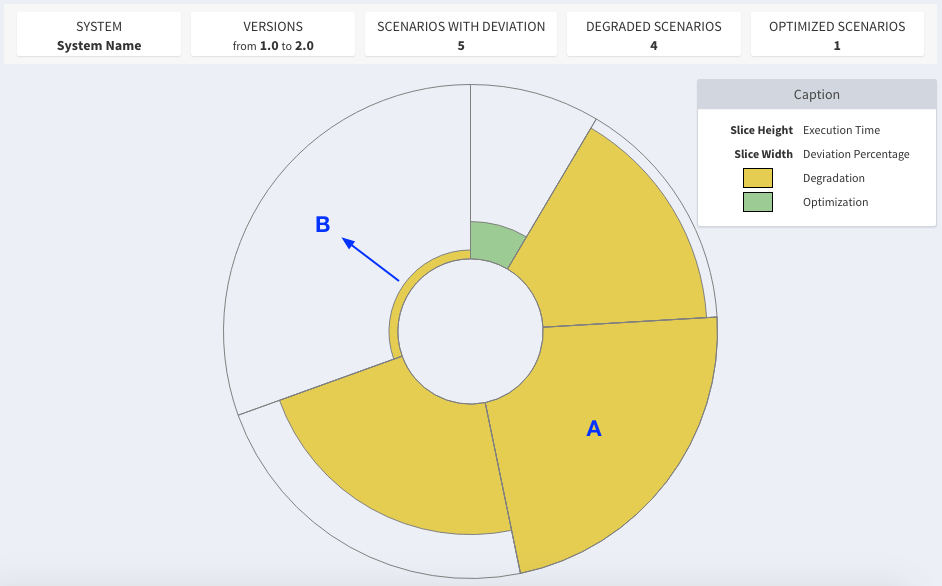
\includegraphics[scale=0.48]{Imagens/sumarizacao_cenarios_visao_geral.png}}
   \textsf{\caption[Visão geral da Sumarização de Cenários.]{Visão geral da Sumarização de Cenários.\label{fig:visualizacao-1-visal-geral}}}
\end{figure}

A partir do gráfico da figura \ref{fig:visualizacao-1-visal-geral}, podem ser vistos 4 cenários com degradação de desempenho e 1 cenário com otimização. Dos cenários com degradação, 3 deles possuem os maiores tempos de execução perante o restante (altura da fatia). A respeito do cenário com otimização, pode-se notar que possui baixo tempo de execução com relação aos demais (altura da fatia) e tem o menor desvio de desempenho com relação à versão anterior analisada (largura da fatia). O cenário indicado pela letra \texttt{A} foi o cenário com maior tempo de execução dentre os analisados, como evidencia a altura da fatia. Já o cenário indicado pela letra \texttt{B} foi o que possuiu a maior variação de desempenho, destacado pela largura da fatia.

\subsection{Interação} \label{subsec:visualizacao1-interacao}

O gráfico desta visualização é passível de ações do usuário, a fim de (i) obter maiores informações sobre determinado cenário ou (ii) avançar para a visualização do grafo de chamadas, descrita mais adiante neste trabalho. Para a primeira ação, o usuário deve posicionar o ponteiro do \textit{mouse} sobre uma das fatias do gráfico e então um \textit{tooltip} é apresentado, como pode ser visto na figura \ref{fig:visualizacao-1-tooltip}.

\begin{figure}[htb]
   \centering
   \frame{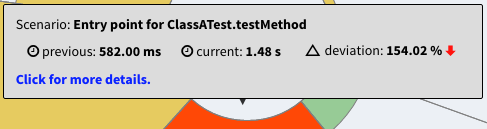
\includegraphics[scale=0.65]{Imagens/sumarizacao_cenarios_tooltip.png}}
   \textsf{\caption[\textit{Tooltip} com maiores informações sobre determinado cenário.]{\textit{Tooltip} com maiores informações sobre determinado cenário.\label{fig:visualizacao-1-tooltip}}}
\end{figure}

No \textit{tooltip} mostrado, é possível verificar o nome do cenário: \texttt{Entry point for ClassA\\Test.testMethod}; o seu tempo de execução na versão anterior: \texttt{582,00 milissegundos}; o tempo de execução na versão atual: \texttt{1,48 segundos}; e a porcentagem de desvio do tempo de execução da versão atual em relação a versão anterior: uma degradação de \texttt{154,02 \%}. É possível concluir que houve uma degradação através da seta vermelha para baixo. Em caso de seta verde para cima, significa que houve uma otimização de desempenho. Ao clicar em uma das fatias do gráfico, o usuário será levado para a visualização do grafo de chamadas.

\subsection{Funcionamento} \label{subsec:sumarizacao-cenarios-funcionamento}

As visualizações apresentadas neste trabalho seguem o mesmo padrão, apresentado na figura \ref{fig:funcionamento-geral-visualizacoes}. Os usuários somente terão acesso às visualizações quando uma análise para a versão desejada já tiver sido processada.

\begin{figure}[!htb]
   \centering
   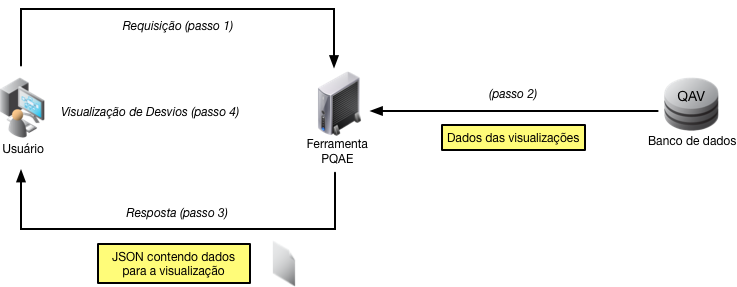
\includegraphics[scale=0.62]{Imagens/funcionamento_geral_visualizacoes.png}
   \textsf{\caption[Funcionamento geral das visualizações.]{Funcionamento geral das visualizações.\label{fig:funcionamento-geral-visualizacoes}}}
\end{figure}

A partir da listagem das análises realizadas na página inicial da aplicação, exibida na figura \ref{fig:pagina-inicial}, o usuário pode clicar no ícone desta visualização (
\includegraphics[height=1.5em,valign=b]{Imagens/visualizacao_1_icone.png}) para acessá-la. Ao clicar, é realizada uma requisição para a aplicação, solicitando acesso à visualização de sumarização de cenários (passo 1). O servidor (Ferramenta PQAE) recebe essa requisição e, a partir dos dados referentes ao sistema e versões desejadas, recupera do banco de dados QAV (passo 2) os dados necessários para a visualização. Após isso, é retornado para o \textit{browser} do usuário um arquivo em formato \abrv[JSON -- \textit{JavaScript Object Notation}]{JSON}(\textit{JavaScript Object Notation}) contendo os dados recuperados (passo 3). O \textit{browser}, por fim, recebe, interpreta esse arquivo e monta a visualização com as devidas informações para que a renderização seja feita com sucesso (passo 4).

O processamento realizado quando o usuário recebe a resposta está exposto na figura \ref{fig:sumarizacao-cenarios-passo-4}. Ao receber o arquivo JSON do servidor, o navegador define a área de desenho que abrigará o gráfico baseado na altura e largura do monitor do usuário. Após isso, é determinado, dentre os cenários indicados pela análise, qual o que possuiu o maior tempo de execução. Esse tempo é utilizado para estabelecer o limite das fatias do gráfico. Isto posto, pelo menos um cenário preencherá por completo uma das fatias do gráfico. Na sequência, a cor, largura e altura, além dos dados do \textit{tooltip} de cada fatia são determinadas baseadas nos dados dos respectivos cenários. Por fim, o gráfico é criado e renderizado.

\begin{figure}[htb]
   \centering
   \frame{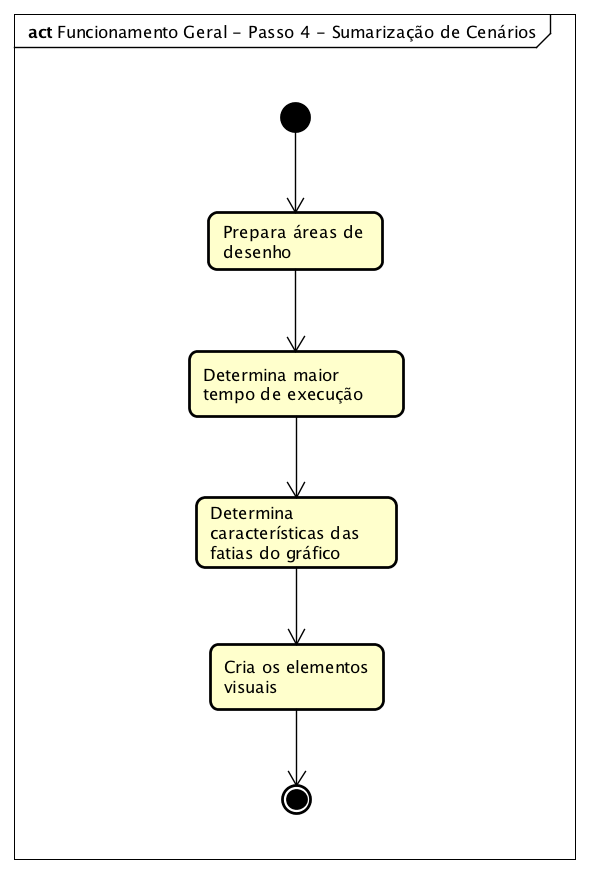
\includegraphics[scale=0.45]{Imagens/sumarizacao_cenarios_passo_4.png}}
   \textsf{\caption[Detalhamento do passo 4 da figura \ref{fig:funcionamento-geral-visualizacoes}, na Sumarização de Cenários.]{Detalhamento do passo 4 da figura \ref{fig:funcionamento-geral-visualizacoes}, na Sumarização de Cenários.\label{fig:sumarizacao-cenarios-passo-4}}}
\end{figure}

\section{Visualização do Grafo de Chamadas} \label{sec:visualizacao2}

Esta visualização tem o objetivo de mostrar, para dadas duas versões de um sistema, os métodos que potencialmente causaram o desvio de desempenho para um determinado cenário. Esses métodos são exibidos em um grafo direcionado de chamadas com propriedades visuais que destacam quais dos métodos mostrados tiveram desvios de desempenho.

Os grafos podem ser utilizados quando os dados a serem representados são estruturados, ou seja, quando existe uma relação inerente entre os elementos de dados a serem visualizados \cite{Herman2000}. Há uma vasta quantidade de áreas onde os grafos podem ser aplicados, por exemplo: hierarquia de arquivos em formato de árvore, mapas de sites, mapas moleculares e genéticos, diagramas de fluxos de dados, entre outros \cite{Herman2000}.

Nesse sentido, em uma chamada de métodos é evidente a relação entre eles, uma vez que os objetos, em um sistema orientado a objetos, trocam mensagens entre si através da invocação dos métodos. O grafo é exibido utilizando o \textit{layout} em árvore, onde os nós filhos estão dispostos abaixo dos nós ancestrais, e a direção dos nós é \textit{top-down}. Um exemplo do grafo é exibido na figura \ref{fig:grafo-chamadas-exemplo}. Nesta seção serão detalhadas as suas propriedades visuais, o seu funcionamento básico, além de descrever a seção de Sumário e Histórico desta visualização.

\begin{figure}[htb]
   \centering
   \frame{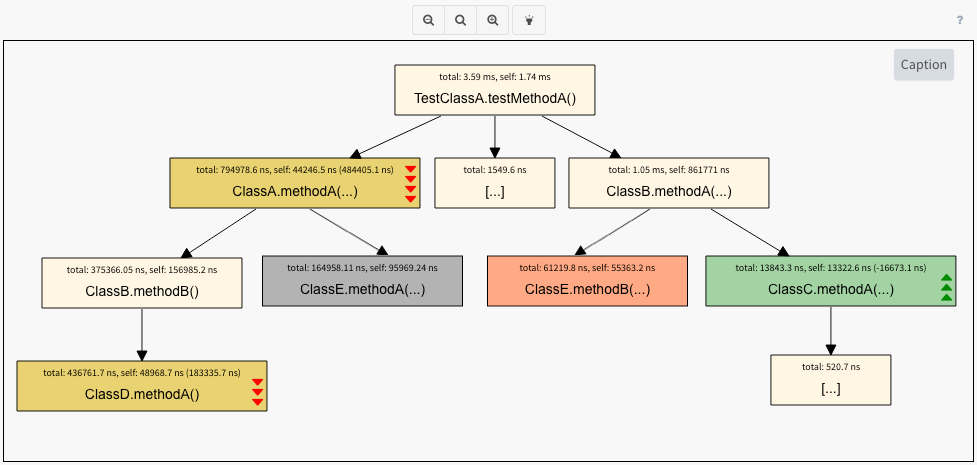
\includegraphics[scale=0.46]{Imagens/grafo_chamadas_exemplo.png}}
   \textsf{\caption[Exemplo do grafo de chamadas.]{Exemplo do grafo de chamadas.\label{fig:grafo-chamadas-exemplo}}}
\end{figure}

\subsection{Sumário} \label{subsubsec:visualizacao2-sumario}

A seção Sumário está disponível acima da seção do Grafo de Chamadas e o seu intuito é trazer outras informações à visualização visando auxiliar os usuários na contextualização do cenário exibido.

\begin{figure}[htb]
   \centering
   \frame{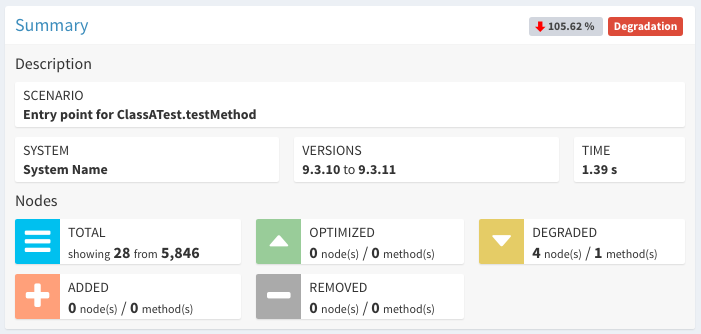
\includegraphics[scale=0.65]{Imagens/grafo_chamadas_sumario.png}}
   \textsf{\caption[Seção de sumário do grafo de chamadas.]{Seção de sumário do grafo de chamadas.\label{fig:grafo-chamadas-sumario}}}
\end{figure}

Na figura \ref{fig:grafo-chamadas-sumario}, é mostrada uma visão geral sobre determinado cenário sendo exibido na visualização. Para a seção \textit{Description}, as informações exibidas são:
\begin{itemize}
   \item \textit{Scenario}: exibe o nome do cenário analisado;
   \item \textit{System}: nome do sistema analisado;
   \item \textit{Versions}: versões do sistema que foram analisadas. É mostrado no formato \textit{<versionA>} to \textit{<versionB>}. Espera-se que a versão B, neste caso, seja posterior a versão A;
   \item \textit{Time}: mostra o tempo de execução do cenário na versão mais recente. A diferença de tempo entre as duas versões vai guiar o que será exibido na barra de títulos da figura. No exemplo mostrado, o tempo na última versão degradou com relação ao tempo na versão anterior, sendo exibido, no canto superior direito, a porcentagem da degradação (\texttt{105,62 \%}) acompanhada de uma seta vermelha para baixo e um rótulo em vermelho marcando o cenário como degradado (\textit{degradation}). Caso o tempo do cenário seja otimizado, é exibida uma seta verde para cima ao lado da porcentagem da variação, além de um rótulo verde marcando o cenário como otimizado (\textit{optimization}).
\end{itemize}

Para a seção \textit{Nodes}, as informações são as seguintes:
\begin{itemize}
   \item \textit{Total}: mostra o número de nós que estão sendo mostrados no grafo de chamadas e total de nós do cenário. Vale salientar que cada nó representa um método executado durante a hierarquia de chamadas do cenário. Pode acontecer de nós diferentes representarem o mesmo método. Isso pode acontecer porque o mesmo método pode ter hierarquias de chamadas diferentes;
   \item \textit{Optimized}: exibe o número de nós e métodos que tiveram otimização de desempenho. Para que um determinado nó seja considerado com otimização de desempenho, ele (i) tem que estar presente nas duas versões analisadas e (ii) o tempo de execução na versão posterior tem que ter sido menor do que na versão anterior;
   \item \textit{Degraded}: exibe o número de nós e métodos que tiveram degradação de desempenho. Para que um determinado nó seja considerado com degradação de desempenho, ele (i) tem que estar presente nas duas versões analisadas e (ii) o tempo de execução na versão posterior tem que ter sido maior do que na versão anterior;
   \item \textit{Added}: apresenta o número de nós e métodos que foram adicionados da versão anterior para a posterior. Ou seja, são os métodos que não existiam na execução do cenário para a versão anterior e passaram a existir na execução da versão posterior. O número de métodos pode ser menor do que o número de nós, uma vez que nós diferentes podem representar o mesmo método;
   \item \textit{Removed}: o contrário do conceito anterior. São apresentados os nós e métodos que foram removidos da versão anterior para a posterior.
\end{itemize}

Para as informações sobre os nós otimizados, degradados, adicionados e removidos, o número de métodos pode ser menor do que o número de nós, uma vez que nós diferentes podem representar o mesmo método se eles estiverem em hierarquias de chamadas diferentes.

\subsection{Histórico} \label{subsubsec:visualizacao2-historico}

A segunda parte da visualização do Grafo de Chamadas apresenta o histórico da evolução do desempenho, em termos de tempo de execução, de determinado cenário. A exibição do histórico é em formato de um gráfico de linha, onde no eixo X são apresentadas as dez últimas versões analisadas em que o cenário esteve presente e no eixo Y é mostrado o tempo de execução. A figura \ref{fig:grafo-chamadas-historico} adiante mostra um exemplo desse gráfico.

\begin{figure}[!htb]
   \centering
   \frame{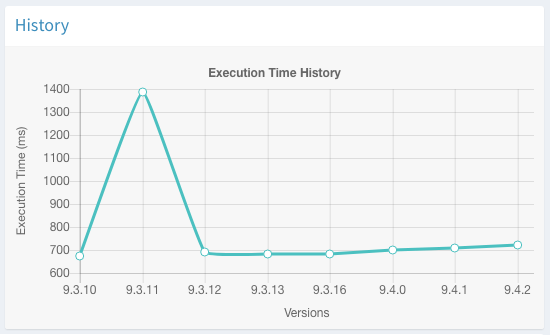
\includegraphics[scale=0.65]{Imagens/grafo_chamadas_historico.png}}
   \textsf{\caption[Seção de histórico do grafo de chamadas.]{Seção de histórico do grafo de chamadas.\label{fig:grafo-chamadas-historico}}}
\end{figure}

Na figura, pode-se concluir que o cenário em questão esteve presente nas versões \texttt{9.3.10}, \texttt{9.3.11}, \texttt{9.3.12}, \texttt{9.3.13}, \texttt{9.3.16}, \texttt{9.4.0}, \texttt{9.4.1} e \texttt{9.4.2}. Entre as versões \texttt{9.3.10} e \texttt{9.3.11}, nota-se uma forte degradação, praticamente duplicando o seu tempo de execução. Por outro lado, da versão \texttt{9.3.11} para a \texttt{9.3.12}, houve uma otimização importante, o que resultou em um tempo de execução próximo ao da versão \texttt{9.3.10}. Da \texttt{9.3.12} a \texttt{9.4.2} pequenas degradações são notadas no desempenho do cenário.

\FloatBarrier % evite que as figuras da subsecao anterior invadam a secao seguinte

\subsection{Grafo de Chamadas} \label{subsubsec:visualizacao2-grafo-chamadas}

A terceira e última parte da visualização é o grafo de chamadas propriamente dito. Esse grafo, como mencionado, é composto de nós e arestas direcionadas que expõem os caminhos das chamadas dos métodos para o cenário analisado. Os nós, representados por caixas, possuem algumas características visuais, apresentadas adiante.

\subsubsection{Nó sem desvio} \label{subsec:no-sem-desvio}

\begin{figure}[htb]
   \centering
   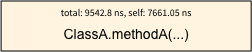
\includegraphics[scale=0.65]{Imagens/no_sem_desvio.png}
   \textsf{\caption[Nó que representa um método sem desvio de desempenho.]{Nó que representa um método sem desvio de desempenho.\label{fig:no-sem-desvio}}}
\end{figure}

O primeiro e mais básico tipo de nó é o que representa um método que não teve desvios de desempenho para o cenário e versões analisadas, apresentado na figura \ref{fig:no-sem-desvio}. As características desse nó são:\tabularnewline
\begin{itemize}
   \item \textit{Cor}: esta é a principal característica que diferencia os nós uns dos outros. No caso deste nó, a cor é marrom claro;
   \item \textit{Nome do nó}: posicionado ao centro, são mostrados o nome da classe e o nome do método executado, no formato \texttt{ClassName.methodName()}. Para otimizar e evitar a exibição de grande quantidade de texto, o nome do pacote e os parâmetros do método foram ocultados, sendo estes, quando houver, representados por três pontos (...). Essa definição serve para todos os tipos de nós dessa visualização;
   \item \textit{Tempos de execução}: localizados no canto superior do nó, são apresentados dois tempos de execução: à esquerda, o tempo total do nó, que representa a soma dos tempos de execução dos nós filhos com o tempo do próprio nó. No exemplo da figura, o tempo total foi de \texttt{9.542,8} nanossegundos; e à direita, o tempo do próprio nó, desconsiderando o tempo dos nós filhos. Na figura, o tempo foi de \texttt{7.661,05} nanossegundos.
   %\item \textit{Detalhes}: no canto superior esquerdo é exibido um ícone onde, ao passar o cursor do \textit{mouse}, o usuário pode obter mais informações sobre o nó. No caso de um nó sem desvio de desempenho, as informações exibidas nesta seção são o nome do pacote e os parâmetros do método, se houver. A figura \ref{fig:detalhes-no-sem-desvio} a seguir mostra essa seção.
\end{itemize}

% \begin{figure}[htb]
%    \centering
%    \frame{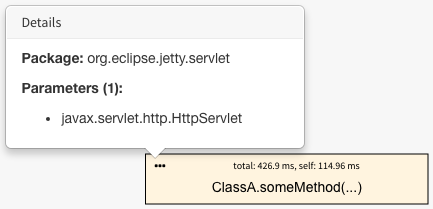
\includegraphics[scale=0.65]{Imagens/detalhes_no_sem_desvio.png}}
%    \textsf{\caption[Seção de detalhes do nó sem desvio de desempenho.]{Seção de detalhes do nó sem desvio de desempenho.\label{fig:detalhes-no-sem-desvio}}}
% \end{figure}

\subsubsection{Nó degradado} \label{subsec:no-degradado}

 A visualização também é capaz de apontar se determinado nó teve o seu desempenho degradado com relação à versão anterior. A figura \ref{fig:no-degradado} apresenta um nó degradado:

\begin{figure}[htb]
   \centering
   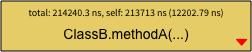
\includegraphics[scale=0.65]{Imagens/no_degradado.png}
   \textsf{\caption[Nó que representa um método com degradação de desempenho.]{Nó que representa um método com degradação de desempenho.\label{fig:no-degradado}}}
\end{figure}

As características visuais deste nó são bem semelhantes às apresentadas para os nós otimizados:
\begin{itemize}
   \item \textit{Cor}: os nós que degradaram o desempenho são mostrados em laranja amarelo;
   \item \textit{Tempos de execução}: além dos tempos total e do próprio nó, um nó com desvio de desempenho, seja otimização ou degradação, apresenta a diferença entre os tempos de execução da versão anterior para a posterior entre parênteses, no canto superior direito. No exemplo da figura, o nó degradou o seu tempo em \texttt{12.202,79} nanossegundos;
   \item \textit{Setas}: no canto inferior direito são mostradas setas indicativas de quão forte ou fraca foi a variação de desempenho. No caso de nós com degradação, são exibidas setas vermelhas apontadas para baixo, onde cada uma delas representa 25\% de desvio do tempo com relação à versão anterior. Sendo assim, uma única seta representa um desvio de 0 a 25\%, duas setas de 25\% a 50\%, três setas de 50\% a 75\% e quatro setas de 75\% ou superior. No exemplo apresentado na figura \ref{fig:no-degradado}, a degradação se deu entre 0 e 25\% do tempo de exeução em relação ao desempenho anterior.
   %\item \textit{Detalhes}: esta seção possui as mesmas informações dos nós relatados até aqui, como podem ser vistas na figura \ref{fig:detalhes-no-degradado} a seguir.
\end{itemize}

% \begin{figure}[htb]
%    \centering
%    \frame{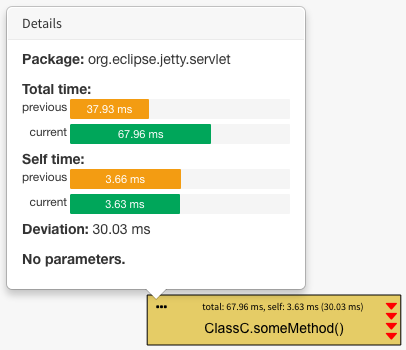
\includegraphics[scale=0.65]{Imagens/detalhes_no_degradado.png}}
%    \textsf{\caption[Seção de detalhes do nó com degradação de desempenho.]{Seção de detalhes do nó com degradação de desempenho.\label{fig:detalhes-no-degradado}}}
% \end{figure}

\subsubsection{Nó otimizado} \label{subsec:no-otimizado}

Quando um cenário possui nós que otimizaram o seu desempenho em relação a versão anterior, outros elementos visuais são acrescidos à visualização. A figura \ref{fig:no-otimizado} a seguir apresenta um nó otimizado:

\begin{figure}[htb]
   \centering
   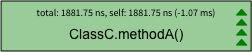
\includegraphics[scale=0.65]{Imagens/no_otimizado.png}
   \textsf{\caption[Nó que representa um método com otimização de desempenho.]{Nó que representa um método com otimização de desempenho.\label{fig:no-otimizado}}}
\end{figure}

As características visuais deste nó, além das comentadas anteriormente, são:
\begin{itemize}
   \item \textit{Cor}: os nós que otimizaram o atributo de qualidade desempenho são mostrados em um tom de verde;
   \item \textit{Tempos de execução}: também são exibidos os tempos de execução total, do próprio nó e o desvio de desempenho. No exemplo, o nó otimizou o tempo em \texttt{1,07} milissegundos;
   \item \textit{Setas}: as setas indicativas de variação de desempenho para nós de otimização são apontadas para cima, de cor verde. No exemplo, a otimização se deu em mais de 75\% do desempenho em relação à versão anteiror.
   %\item \textit{Detalhes}: esta seção para os nós com otimização de desempenho possui informações diferentes das relatadas anteriormente, como podem ser vistas na figura \ref{fig:detalhes-no-otimizado}. Além das informações sobre o pacote e os parâmetros, também são apresentadas sobre os tempos de execução da versão anterior e posterior, além da variação de tempo.
\end{itemize}

%\begin{figure}[htb]
%    \centering
%    \frame{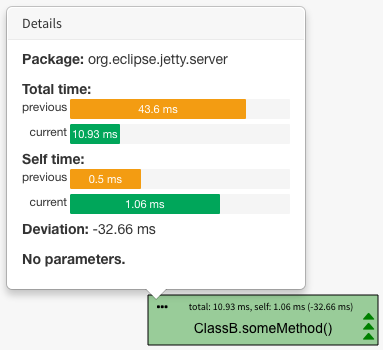
\includegraphics[scale=0.65]{Imagens/detalhes_no_otimizado.png}}
%    \textsf{\caption[Seção de detalhes do nó com otimização de desempenho.]{Seção de detalhes do nó com otimização de desempenho.\label{fig:detalhes-no-otimizado}}}
% \end{figure}

\subsubsection{Nó adicionado} \label{subsec:no-adicionado}

Um cenário pode apresentar, para diferentes versões, nós de chamadas de métodos que estão presentes na versão atual, mas que não existiam na versão anterior: são os nós adicionados. A visualização representa esses nós como mostra a figura \ref{fig:no-adicionado}. A descrição dos atributos visuais é a que segue:

\begin{figure}[htb]
   \centering
   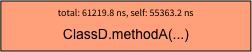
\includegraphics[scale=0.65]{Imagens/no_adicionado.png}
   \textsf{\caption[Nó que representa um método adicionado.]{Nó que representa um método adicionado.\label{fig:no-adicionado}}}
\end{figure}

\begin{itemize}
   \item \textit{Cor}: os nós que foram adicionados na versão atual são mostrados na cor salmão claro;
   \item \textit{Tempos de execução}: os tempos de execução total e do próprio nó são exibidos. No exemplo, o tempo total do nó é de \texttt{61.219,8} nanossegundos e o tempo do próprio nó é de \texttt{55.363,2} nanossegundos.
   %\item \textit{Detalhes}: nos nós adicionados, os detalhes possuem as mesmas informações exibidas para os nós de degradação ou de otimização. No entanto, uma mensagem é exibida em vermelho indicando que o nó adicionado é um potencial causador da degradação de desempenho do cenário. A figura \ref{fig:detalhes-no-adicionado} adiante apresenta esta seção.
\end{itemize}

% \begin{figure}[htb]
%    \centering
%    \frame{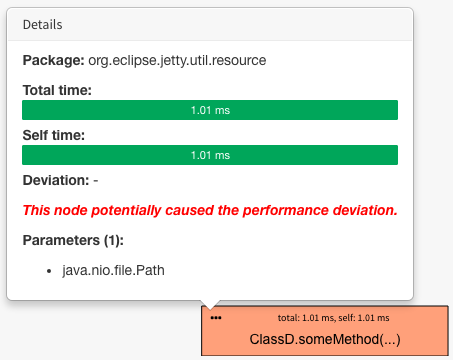
\includegraphics[scale=0.65]{Imagens/detalhes_no_adicionado.png}}
%    \textsf{\caption[Seção de detalhes do nó adicionado.]{Seção de detalhes do nó adicionado.\label{fig:detalhes-no-adicionado}}}
% \end{figure}

\subsubsection{Nó removido} \label{subsec:no-removido}

De maneira contrária ao que foi relatado sobre o nó adicionado, um cenário pode não possuir, na versão atual, chamadas de métodos que estavam presentes na versão anterior. Significa que essas chamadas, para a hierarquia de chamadas de métodos do cenário, foram removidas. No entanto, vale salientar que esse fato não representa que o método em si (código-fonte) foi removido. A figura \ref{fig:no-removido} mostra a representação de um nó removido no grafo. A descrição dos atributos visuais é a que segue:

\begin{figure}[htb]
   \centering
   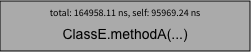
\includegraphics[scale=0.65]{Imagens/no_removido.png}
   \textsf{\caption[Nó que representa um método removido.]{Nó que representa um método removido.\label{fig:no-removido}}}
\end{figure}

\begin{itemize}
   \item \textit{Cor}: os nós que foram removidos na versão atual possuem cor em um tom de cinza;
   \item \textit{Tempos de execução}: os tempos de execução total e do próprio nó na versão anterior são exibidos. No exemplo, o tempo total do nó é de \texttt{164.958,11} nanossegundos e o tempo do próprio nó é de \texttt{95.969,24} nanossegundos.
\end{itemize}

\subsubsection{Nó de agrupamento} \label{subsec:no-agrupamento}

Além dos que representam métodos com ou sem desvio de desempenho, e métodos adicionados e removidos, há um tipo de nó que representa um agrupamento de vários outros: o agrupado. Assim, os que não estão diretamente relacionados com nós de desvio, adicionados ou removidos, são omitidos e representados por um único nó agrupado. A figura \ref{fig:no-agrupamento} a seguir ilustra esse tipo de nó, seguido da descrição dos seus atributos visuais.

\begin{figure}[htb]
   \centering
   \frame{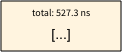
\includegraphics[scale=0.65]{Imagens/no_agrupado.png}}
   \textsf{\caption[Nó que representa um agrupamento de outros nós.]{Nó que representa um agrupamento de outros nós.\label{fig:no-agrupamento}}}
\end{figure}

\begin{itemize}
   \item \textit{Cor}: os nós de agrupamento são mostrados na cor marrom claro;
   \item \textit{Nome do nó}: posicionado ao centro, é exibido o texto \textit{[...]};
   \item \textit{Tempos de execução}: é exibido o tempo de execução total que representa a soma de todos os tempos de execução dos nós contidos no agrupamento. No exemplo, o tempo total é de \texttt{527,3} nanossegundos.
\end{itemize}

Cada nó no grafo de chamadas, da forma como foi apresentado até o momento, representa uma única execução deste. No entanto, um nó, para determinada hierarquia de chamadas, pode ser executado mais de uma vez (por exemplo, em um \textit{loop}). Com o intuito de não acrescentar nós ao grafo para representar essas situações, foi estabelecido que se um nó possuir uma borda espessa, significa que este executou mais de uma vez naquela hierarquia. A figura \ref{fig:no-borda-espessa} adiante exemplifica um nó com uma borda espessa.

\begin{figure}[htb]
   \centering
   \frame{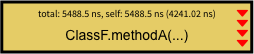
\includegraphics[scale=0.65]{Imagens/no_borda_espessa.png}}
   \textsf{\caption[Borda espessa de um nó, representando múltiplas execuções.]{Borda espessa de um nó, representando múltiplas execuções.\label{fig:no-borda-espessa}}}
\end{figure}

As propriedades visuais apresentadas para a visualização do grafo de chamadas incluem, em suma, três partes: (i) seção de sumário, contendo informações gerais sobre o cenário; (ii) seção de histórico, mostrando o histórico do desempenho do cenário dentre as dez últimas versões analisadas; e (iii) seção do grafo de chamadas, onde a execução dos métodos é representada através de nós e arestas. Esta seção é a mais importante desta visualização, contendo características visuais que diferem os nós de acordo com sua classificação. Um resumo dessas características é apresentado na tabela \ref{tab:resumo-caracteristicas-nos} a seguir.

\begin{table}[!htb]
   \textsf{\caption{Resumo das características visuais dos nós.\label{tab:resumo-caracteristicas-nos}}}
   \centering
   \medskip
   \begin{tabular}{c|c|c|c|c}
   \textbf{Tipo} & \textbf{Cor}   & \textbf{\begin{tabular}[c]{@{}c@{}}Tempos de\\ Execução\end{tabular}} & \textbf{Setas} \\ \hline
   Sem desvio    & Marrom claro   & Total e próprio                                                       & Sem setas \\ \hline
   Degradado     & Vermelho claro & \begin{tabular}[c]{@{}c@{}}Total, próprio\\ e desvio\end{tabular}     & \begin{tabular}[c]{@{}c@{}}Vermelhas,\\ para baixo\end{tabular} \\ \hline
   Otimizado     & Verde claro    & \begin{tabular}[c]{@{}c@{}}Total, próprio\\ e desvio\end{tabular}     & \begin{tabular}[c]{@{}c@{}}Verdes,\\ para cima\end{tabular} \\ \hline
   Adicionado    & Salmão claro   & Total e próprio                                                       & Sem setas \\ \hline
   Removido    & Cinza   & Total e próprio                                                       & Sem setas \\ \hline
   Agrupado      & Marrom claro   & Total                                                                 & Sem setas
   \end{tabular}
\end{table}

\subsection{Interação} \label{subsec:interacao-grafo-chamadas}

Esta visualização exibe um conjunto de informações que a torna capaz de indicar os métodos que potencialmente foram responsáveis por desvios de desempenho de um determinado cenário. Contudo, o usuário pode interagir com o grafo efetuando o efeito de zoom, destacando o caminho de execução de determinado nó com desvio ou obtendo mais informações sobre um nó passando o cursor do \textit{mouse} sobre ele.

O zoom pode ser acessado pela barra de ferramentas mostrada na figura \ref{fig:grafo-chamadas-barra-ferramentas}. Essa barra situa-se logo acima da área de desenho do grafo (como pode ser visto na figura \ref{fig:grafo-chamadas-exemplo}) e exibe os botões marcados de \texttt{A} a \texttt{D}. Os botões \texttt{A}, \texttt{B} e \texttt{C} podem ser clicados para realizar o efeito de zoom. O botão A realiza o efeito de distanciamento (\textit{Zoom Out}), o botão B redefine o zoom para o estado inicial (100\%) e o botão C efetua o efeito de aproximação (\textit{Zoom In}). O zoom pode fazer com que o grafo seja comportado novamente na área de desenho.

\begin{figure}[htb]
   \centering
   \frame{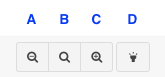
\includegraphics[scale=0.70]{Imagens/grafo_chamadas_barra_ferramentas.png}}
   \textsf{\caption[Barra de ferramentas do grafo de chamadas.]{Barra de ferramentas do grafo de chamadas.\label{fig:grafo-chamadas-barra-ferramentas}}}
\end{figure}

O destaque do caminho de execução de um nó com desvio esmaece todos os nós que não estão no caminho de execução do nó desejado. Existem duas formas de se obter esse efeito: a primeira delas é a partir do botão \texttt{D} da barra de ferramentas. Esse botão, ao ser clicado, destaca os caminhos para todos os nós com desvio mostrados no grafo, como exemplifica a figura \ref{fig:grafo-chamadas-destaque}. Para desfazer o efeito, o botão deve ser clicado novamente; a segunda forma de se obter esse destaque é efetuando um duplo clique em algum dos nós com desvio exibido no grafo. Isso fará com que o caminho do nó raiz até o nó clicado seja destacado, esmaecendo todos os outros. Para reverter o efeito, nessa situação, o usuário pode realizar o duplo clique em qualquer nó sem desvio de desempenho exibido no grafo.

\begin{figure}[htb]
   \centering
   \frame{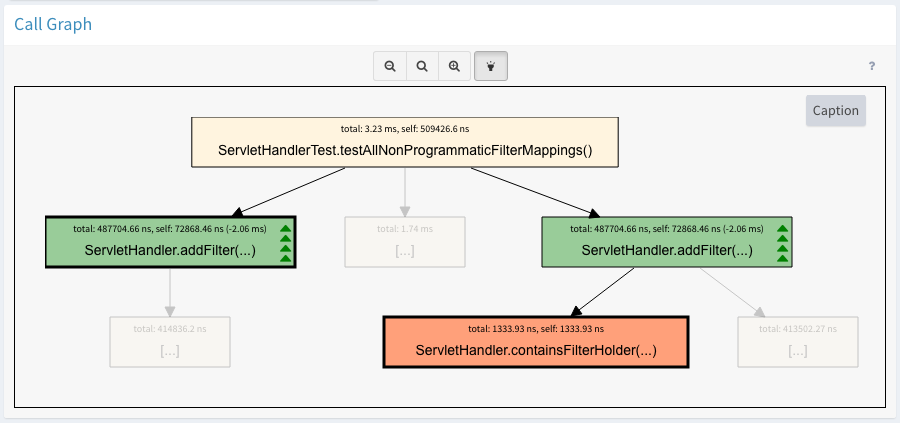
\includegraphics[scale=0.50]{Imagens/grafo_chamadas_destaque.png}}
   \textsf{\caption[Efeito de destaque do caminho de execução de nós com desvio.]{Efeito de destaque do caminho de execução de nós com desvio.\label{fig:grafo-chamadas-destaque}}}
\end{figure}

Uma legenda explicativa também foi implementada para ajudar na interpretação do grafo. O usuário pode acessá-la clicando no botão \texttt{Caption}, no canto superior direito do grafo. Ao ser clicada, a legenda é expandida, exibindo os elementos visuais e seus significados, conforme mostrado na figura \ref{fig:grafo-chamadas-legenda}.

\begin{figure}[htb]
   \centering
   \frame{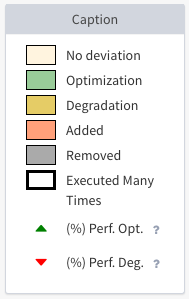
\includegraphics[scale=0.65]{Imagens/grafo_chamadas_legenda.png}}
   \textsf{\caption[Legenda do grafo de chamadas.]{Legenda do grafo de chamadas.\label{fig:grafo-chamadas-legenda}}}
\end{figure}

O usuário pode obter mais detalhes sobre cada nó exibido no grafo. Para isso, ele deve posicionar o ponteiro do mouse sobre o nó desejado e aguardar meio segundo. Após esse tempo, é exibido um \textit{tooltip} com essas informações. A figura \ref{fig:grafo-chamadas-detalhes-no} exemplifica os detalhes de um nó.

\begin{figure}[htb]
   \centering
   \frame{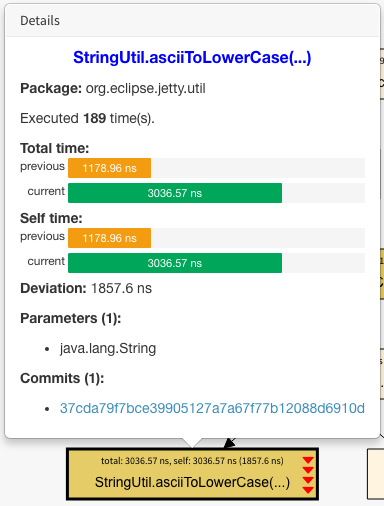
\includegraphics[scale=0.55]{Imagens/grafo_chamadas_detalhes_no.png}}
   \textsf{\caption[Detalhes de um nó no grafo de chamadas.]{Detalhes de um nó no grafo de chamadas.\label{fig:grafo-chamadas-detalhes-no}}}
\end{figure}

Na figura, podem ser encontradas informações sobre o pacote do método representado, a quantidade de vezes que o nó foi executado em caso de execução múltipla, o tempo total na versão anterior e atual, o tempo do próprio nó na versão anterior e atual, o tempo de desvio de desempenho, a listagem de parâmetros do método e a listagem de \textit{commits} que possivelmente causaram o desvio de desempenho do nó. Dependendo do tipo de nó ao qual se quer obter os detalhes, podem existir mais ou menos as informações a serem apresentadas.

\FloatBarrier % evite que as figuras da subsecao anterior invadam a secao seguinte

\subsection{Funcionamento} \label{subsec:funcionamento-visualizacao-2}

Após a execução de uma nova análise, conforme apresentado na seção \ref{subsec:new-analysis}, o funcionamento desta visualização segue o funcionamento geral das visualizações mostrado na figura \ref{fig:funcionamento-geral-visualizacoes}, no entanto, no passo 4 dessa figura, existem processamentos específicos a fim de tratar os dados antes de serem exibidos para o usuário.

Seguindo o fluxo da figura \ref{fig:funcionamento-geral-visualizacoes}, a partir da visualização de sumarização de cenários, o usuário pode clicar em uma das fatias daquele gráfico e realizar uma requisição para a visualização do grafo de chamadas (passo 1). O servidor recebe essa requisição e, a partir dos parâmetros enviados, recupera do banco de dados QAV (passo 2) os dados necessários para a visualização. Após isso, é retornado para o navegador do usuário um arquivo em formato JSON contendo os dados recuperados (passo 3). O navegador, por fim, recebe, interpreta esse arquivo e monta a visualização com as devidas informações para que a renderização seja feita com sucesso (passo 4).

No passo 4 da figura \ref{fig:funcionamento-geral-visualizacoes}, há um procedimento executado no navegador do usuário que recebe e processa o arquivo JSON e, ao final, renderiza o grafo de chamadas. Esse processo está exposto em detalhes na figura \ref{fig:grafo-chamadas-passo-4} adiante. O início ocorre ao receber o arquivo do servidor e a primeira atividade é criar a área de desenho que abrigará o grafo. Nessa atividade são considerados a altura e largura do monitor do usuário, de modo que a área útil de apresentação seja compatível com a área do monitor.

\begin{figure}[!htb]
   \centering
   \frame{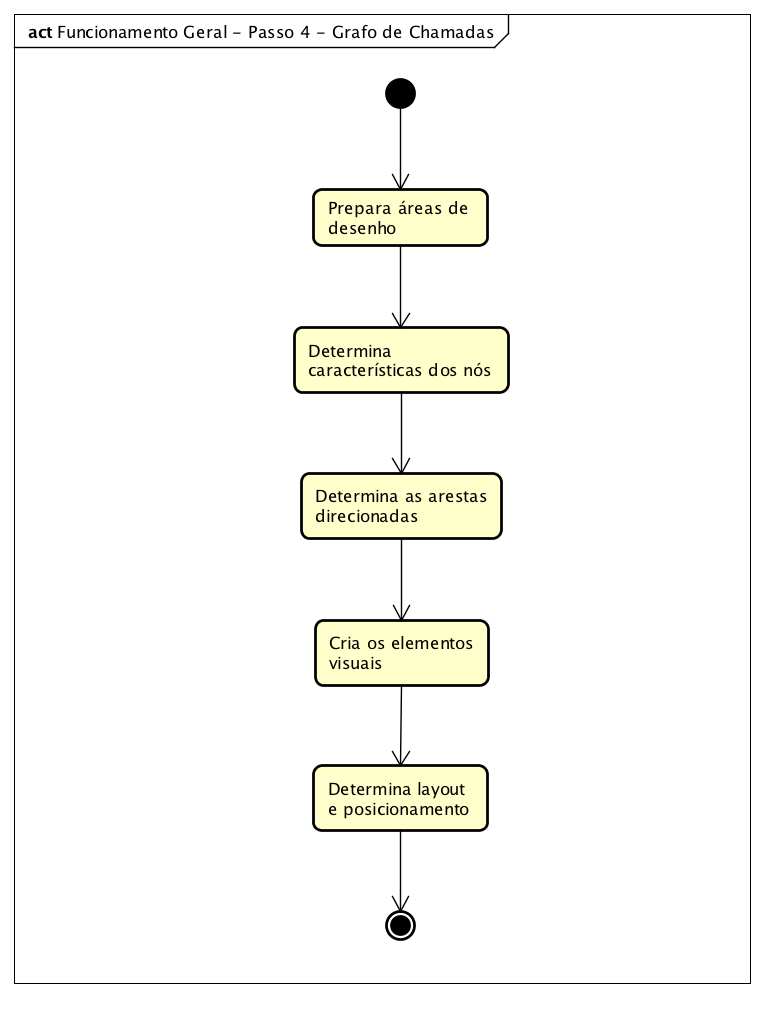
\includegraphics[scale=0.50]{Imagens/grafo_chamadas_passo_4.png}}
   \textsf{\caption[Detalhamento do passo 4 da figura \ref{fig:funcionamento-geral-visualizacoes}, no Grafo de Chamadas.]{Detalhamento do passo 4 da figura \ref{fig:funcionamento-geral-visualizacoes}, no Grafo de Chamadas.\label{fig:grafo-chamadas-passo-4}}}
\end{figure}

Após isso, as características dos nós contidos no arquivo JSON são determinadas. Para cada um deles, são determinados: (i) a altura e largura da sua caixa, que é diretamente proporcional ao tamanho do nome a ser exibido. Vale salientar que o pacote da classe é omitido para a exibição do nome; (ii) a espessura da borda, caso o nó tenha sido executado mais de uma vez; (iii) a cor, que depende do seu tipo; (iv) os tempos de execução total e, caso pertinente, o do próprio nó e o de desvio; (v) as setas, que dependem do seu tipo e da porcentagem de desvio do tempo de execução ocorrida de uma versão para outra; e (vi) os detalhes a serem exibidos no \textit{tooltip}, que dependem do tipo do nó.

Depois, as arestas são determinadas de acordo com a relação de nós pais e filhos contidos no arquivo. Elas são direcionadas do nó pai para os filhos, indicando a hierarquia de chamadas.

Com a definição dos nós e suas características, e das arestas, a próxima atividade do processo é criar os elementos visuais na área de desenho, para, posteriormente, determinar o \textit{layout} (conforme citado anteriormente, o \textit{layout} utilizado é em árvore) e posicionamento dos nós. Por fim, o grafo de chamadas é renderizado para o usuário.

\subsection{Exemplo de Uso da Ferramenta: Jetty {\color{red}fica ou sai?}} \label{subsec:exemplo-uso-jetty}

Foi realizado um estudo de caso para exemplificar o uso das visualizações. Para tanto, foi utilizado duas versões da aplicação Jetty \cite{Jetty2016}: 9.2.6 e 9.3.0.M1. Esse sistema faz parte do Projeto Eclipse e é um \textit{framework open-source} que provê um servidor web além de um servlet container Java. Essa aplicação foi escolhida para o estudo de caso pois todos os tipos de nós foram capazes de ser exemplificados.

Para a primeira fase do \textit{\perfMinerName}, a análise dinâmica, todos os testes automatizados foram considerados cenários. Como os testes são implementados em JUnit 4, o aspecto interceptou todos os métodos marcados com a anotação \texttt{@Test} como métodos de entrada de um cenário. A análise dinâmica, como mencionado anteriormente, foi executada no mesmo computador para ambas as versões, nas mesmas condições e com todos os serviços não essenciais desabilitados. A suíte de testes do Jetty foi executada 30 vezes para que as medições de desempenho fossem mais precisas em termos de tempo de execução \cite{Pinto2015}.

A resultado da análise foi um total de 11 cenários, sendo 7 com degradação do desempenho e 4 com otimização. No grafo gerado, é possível que dois nós representem o mesmo método, indicando duas execuções, e as arestas direcionadas representam invocações entre os métodos. A figura \ref{fig:exemplo-degradacao} exemplifica o grafo de um cenário com degradação.

\begin{figure}[!htb]
   \centering
   \frame{\includegraphics[scale=0.52]{Imagens/exemplo_degradacao.png}}
   \textsf{\caption[Grafo de chamadas de um cenário com degradação de desempenho.]{Grafo de chamadas de um cenário com degradação de desempenho.\label{fig:exemplo-degradacao}}}
\end{figure}

O grafo exibido destaca que o nó raiz, \texttt{DefaultServletTest.testFiltered()}, teve uma degradação de desempenho de mais de 75\%, indicado pela cor do nó, laranja amarelo, e pelas quatro setas vermelhas para baixo. É possível notar também que dois nós que representam o método \texttt{Server.doStart()} foram adicionados. Isso significa que durante a execução do cenário \texttt{Entry point for DefaultServletTest.testFiltered} duas chamadas a esse método foram efetuadas na versão 9.3.0.M1, e elas não existiam na versão 9.3.6. Os nós adicionados são indicados como potenciais causadores de degradação de desempenho, de modo que, possivelmente, esses nós influenciaram na degradação do raiz. Na visualização há nós que não têm relação com os desvios, representados como agrupados, e nós sem desvio, representados na cor marrom claro.

Na mesma figura, além do próprio grafo, na parte superior da seção \textit{Call Graph} é encontrada uma barra de ferramentas com botões de \textit{Zoom Out}, \textit{Zoom to Fit} e \textit{Zoom In}; e na parte inferior é exibida uma legenda ajudando os usuários a identificarem os nós do grafo. Os botões de \textit{zoom} e a legenda são exibidos para todos os grafos, independente da quantidade de nós ou do tipo de desvio ocorrido.

Na figura \ref{fig:exemplo-detalhes-degradacao} adiante, a seção \textit{Details} desse cenário é exibida expandida, indicando, no rótulo, que o cenário teve o seu desempenho degradado entre as versões, e que o total de nós para esse cenário foi de 1695.

\begin{figure}[!htb]
   \centering
   \frame{\includegraphics[scale=0.48]{Imagens/exemplo_detalhes_degradacao.png}}
   \textsf{\caption[Detalhes de um cenário com degradação de desempenho.]{Detalhes de um cenário com degradação de desempenho.\label{fig:exemplo-detalhes-degradacao}}}
\end{figure}

A figura \ref{fig:exemplo-otimizacao} a seguir apresenta o cenário \texttt{Entry point for ServletContextHandler\\Test.testFallThrough} com otimização de desempenho. Dois nós contribuíram para esse desvio, identificados pela cor verde claro: \texttt{Server.doStart()} e \texttt{ServletContextHandler.\\relinkHandlers()}. No primeiro, a variação foi entre 50\% e 75\%, ao passo que no segundo foi de mais de 75\%. Há ainda a representação de nós agrupados e sem desvio.

\begin{figure}[!htb]
   \centering
   \frame{\includegraphics[scale=0.52]{Imagens/exemplo_otimizacao.png}}
   \textsf{\caption[Grafo de chamadas de um cenário com otimização de desempenho.]{Grafo de chamadas de um cenário com otimização de desempenho.\label{fig:exemplo-otimizacao}}}
\end{figure}

\begin{figure}[!htb]
   \centering
   \frame{\includegraphics[scale=0.48]{Imagens/exemplo_detalhes_otimizacao.png}}
   \textsf{\caption[Detalhes de um cenário com otimização de desempenho.]{Detalhes de um cenário com otimização de desempenho.\label{fig:exemplo-detalhes-otimizacao}}}
\end{figure}

A seção \textit{Details} expandida pode ser vista na figura \ref{fig:exemplo-detalhes-otimizacao}. O rótulo de otimização é exibido no canto superior esquerdo indicando o tipo de desvio ocorrido no cenário. A figura indica um total de 986 nós para esse cenário.

% A tabela \ref{tab:jetty-v9.2.6-v9.3.0.M1} a seguir mostra uma lista com todos os cenários para o sistema Jetty, versões 9.2.6 para 9.3.0.M1. Nela, são exibidas as porcentagens de desvio de degradação ou otimização para os cenários.

% \begin{sidewaystable}[!htb]
%    \textsf{\caption{Cenários para o Jetty, versões 9.2.6 para 9.3.0.M1.\label{tab:jetty-v9.2.6-v9.3.0.M1}}}
%    \centering
%    \medskip
%    \begin{tabular}{l|c|c|c|c}
%    \multicolumn{1}{c|}{\textbf{Nome}}                                                                                                       & \textbf{\begin{tabular}[c]{@{}c@{}}Tempo \\ v9.2.6 (ms)\end{tabular}} & \textbf{\begin{tabular}[c]{@{}c@{}}Tempo \\ v9.3.0.M1 (ms)\end{tabular}} & \textbf{\begin{tabular}[c]{@{}c@{}}Variação \\ (\%)\end{tabular}} & \textbf{\begin{tabular}[c]{@{}c@{}}Tipo de \\ Desvio\end{tabular}} \\ \hline
%    \begin{tabular}[c]{@{}l@{}}Entry point for \\ DispatcherForwardTest.testQueryRetainedByForward\\ WithoutQuery\end{tabular}              & 569,26                                                                & 597,33                                                                   & 4,93                                                              & Degradação                                                         \\ \hline
%    \begin{tabular}[c]{@{}l@{}}Entry point for \\ SSLAsyncIOServletTest.testAsyncIOWritesWith\\ Aggregation\end{tabular}                    & 549,21                                                                & 587,55                                                                   & 6,98                                                              & Degradação                                                         \\ \hline
%    \begin{tabular}[c]{@{}l@{}}Entry point for \\ AsyncServletLongPollTest.testSuspendedRequest\\ CompletedByAnotherRequest\end{tabular}    & 620,36                                                                & 634,60                                                                   & 2,29                                                              & Degradação                                                         \\ \hline
%    Entry point for DefaultServletTest.testFiltered                                                                                         & 37,93                                                                 & 67,96                                                                    & 79,17                                                             & Degradação                                                         \\ \hline
%    \begin{tabular}[c]{@{}l@{}}Entry point for \\ ServletContextHandlerTest.testReplaceServlet\\ HandlerWithoutServlet\end{tabular}         & 429,60                                                                & 453,96                                                                   & 5,67                                                              & Degradação                                                         \\ \hline
%    \begin{tabular}[c]{@{}l@{}}Entry point for \\ AsyncContextListenersTest.testAsyncDispatch\\ AsyncCompletePreservesListener\end{tabular} & 601,83                                                                & 622,96                                                                   & 3,51                                                              & Degradação                                                         \\ \hline
%    \begin{tabular}[c]{@{}l@{}}Entry point for \\ AsyncIOServletTest.testAsyncWriteThrowsError\end{tabular}                                 & 599,10                                                                & 611,00                                                                   & 1,98                                                              & Degradação                                                         \\ \hline
%    \begin{tabular}[c]{@{}l@{}}Entry point for \\ DispatcherForwardTest.testQueryAggregatesWith\\ FormByForwardWithoutQuery\end{tabular}    & 26,46                                                                 & 20,76                                                                    & 21,54                                                             & Otimização                                                         \\ \hline
%    \begin{tabular}[c]{@{}l@{}}Entry point for \\ ServletContextHandlerTest.testFallThrough\end{tabular}                                    & 52,00                                                                 & 19,23                                                                    & 63,01                                                             & Otimização                                                         \\ \hline
%    \begin{tabular}[c]{@{}l@{}}Entry point for \\ AsyncContextListenersTest.testListenerCleared\\ OnSecondRequest\end{tabular}              & 23,90                                                                 & 17,16                                                                    & 28,20                                                             & Otimização                                                         \\ \hline
%    \begin{tabular}[c]{@{}l@{}}Entry point for \\ ServletContextHandlerTest.testAddServletAfterStart\end{tabular}                           & 55,56                                                                 & 20,40                                                                    & 63,28                                                             & Otimização                                                     
%    \end{tabular}
% \end{sidewaystable}

%A maior variação absoluta foi para o cenário \texttt{Entry point for DefaultServletTest\\.testFiltered}, uma degradação de 79,17\%. Como destacado na figura \ref{fig:exemplo-degradacao}, dois nós com tempos significantes com relação ao cenário foram adicionados, provavelmente, causando a degradação. O gráfico \ref{fig:grafico-jetty-v9.2.6-v9.3.0.M1} adiante exibe a porcentagem de variação de desempenho.

% \begin{sidewaysfigure}[!htb]
%    \centering
%    \frame{\includegraphics[scale=0.80]{Imagens/grafico_jetty_v926_v931M1.png}}
%    \textsf{\caption[Porcentagem de desvios de desempenho para o Jetty, versões 9.2.6 para 9.3.0.M1.]{Porcentagem de desvios de desempenho para o Jetty, versões 9.2.6 para 9.3.0.M1.\label{fig:grafico-jetty-v9.2.6-v9.3.0.M1}}}
% \end{sidewaysfigure}

\section{Considerações} \label{sec:consideracoes-cap3}

Um dos principais desafios do processo de manutenção de um software é compreendê-lo adequadamente, em especial, a sua arquitetura. A falta de acompanhamento da evolução da arquitetura ao longo do tempo pode levar a sua degradação, impactando os seus atributos de qualidade. Este capítulo apresentou visualizações de arquitetura de software que visam tornar direta e fácil a monitoração da evolução arquitetural, com relação ao atributo de qualidade de desempenho. Uma vez que as ferramentas existentes se mostram complexas ou ineficientes para essa finalidade, as visualizações foram propostas a serem implementadas como extensões da ferramenta \textit{\perfMinerName}. Em suma, são as seguintes:
\begin{enumerate}[(i)]
   \item \textit{Sumarização dos Cenários}: a sumarização dos cenários com desvio de desempenho objetiva mostrar, de maneira sucinta, quais cenários analisados tiveram desvio de desempenho, seja degradação ou otimização;
   \item \textit{Grafo de Chamadas}: a visualização do grafo de chamadas exibe, para cada cenário, as chamadas dos métodos que tiveram desvio de desempenho. Dessa forma, o usuário pode localizar em qual trecho de código da execução do cenário houve o desvio.
\end{enumerate}

A visualização da sumarização de cenários permite aos usuários ter uma visão geral de todos os cenários indicados com desvios de desempenho entre uma determinada versão e a anterior. A visualização mostra os cenários em um gráfico de rosca, onde cada cenário é representado por uma fatia dessa rosca, e todos os cenários compõem a integralidade do gráfico. Dessa forma, os usuários podem identificar se os cenários exibidos são de degradação ou otimização, identificar o cenário com maior tempo de execução dentre os exibidos e o que possuiu a maior porcentagem de desvio de desempenho.

Foi mostrado os detalhes da visualização do grafo de chamadas, que visa exibir, para dadas duas versões de um sistema, os métodos que potencialmente causaram o desvio de desempenho para um determinado cenário. Nesta visualização, os métodos são apresentados em um grafo direcionado de chamadas com propriedades visuais que destacam quais dos métodos mostrados tiveram desvios de desempenho. Com essa visualização, os usuários podem identificar as possíveis causas de desvios de desempenho em determinado cenário através da listagem de \textit{commits} presentes em cada nó com desvio de desempenho, adicionado ou removido.
	
	% Capitulo 4: Quarto capítulo (arquivo Includes/Capitulo4.tex)
	% Capíulo 4
\chapter{Avaliação} \label{ch:avaliacao}

Este capítulo descreve o estudo empírico realizado em dois sistemas \textit{open-source} de diferentes domínios cujo objetivo é avaliar se as visualizações são úteis para representar os desvios de desempenho encontrados durante a análise desses sistemas, além de avaliar a facilidade de se encontrar informações e a possível aplicabilidade da ferramenta como parte integrande dos processos de desenvolvimento dos sistemas analisados.

O restante deste capítulo está organizado como segue: seção \ref{sec:avaliacao-projeto} apresenta como o estudo foi projetado, incluindo as principais contribuições (subseção \ref{subsec:avaliacao-principais-contribuicoes}), os objetivos e questões de pesquisa (subseção \ref{subsec:avaliacao-objetivos-questoes-pesquisa}), os sistemas analisados (subseção \ref{subsec:avaliacao-sistemas}) e os procedimentos do estudo (subseção \ref{subsec:avaliacao-procedimentos}); a seção \ref{sec:avaliacao-resultados} exibe os resultados do estudo e a seção \ref{sec:avaliacao-consideracoes} conclui o capítulo, apresentando as ameaças à validade e discussões sobre os resultados.

\section{Projeto} \label{sec:avaliacao-projeto}

O estudo analisou um total de 20 releases dos projetos Jetty \cite{Jetty2016} e VRaptor \cite{VRaptor2017}, sendo 10 releases para cada sistema, considerando 193 cenários distintos ao total, gerando as visualizações de sumarização dos cenários e grafo de chamadas para todos os casos. Sobre as visualizações, foram coletados feedback de usuários desses sistemas através de um questionário online.

De maneira geral, foram aplicadas as fases discutidas no capítulo \ref{ch:pqae}, subseção \ref{subsec:funcionamento-perfminer}, além do procedimento necessário para gerar os dados para as visualizações, conforme descrito na seção \ref{sec:visao-geral-architecture-qa-evolution} do mesmo capítulo. Em suma: (i) primeiro, os casos de testes automatizados (cada um deles representando um cenário) dos sistemas foram executados e monitorados, resultando em múltiplos bancos de dados; (ii) depois, os dados coletados foram comparados, agrupando releases subsequentes para cada sistema; (iii) então, os elementos identificados com desvios de desempenho foram minerados nos seus sistemas de controle de versão, com o intuito de descobrir os \textit{commits} que alteraram esses artefatos; (iv) por fim, foi executado, para cada versão de cada sistema, o procedimento necessário para gerar os dados que dão suporte às visualizações. Após isso, o questionário online foi elaborado e aplicado.

O questionário foi enviado para todos os contribuidores dos sistemas que possuiam endereço de email registrado na página de contribuidores de cada sistema ou na página do seu perfil. Dos 114 contribuidores que receberam o questionário, 16 deles responderam com algum feedback.

\subsection{Principais Contribuições} \label{subsec:avaliacao-principais-contribuicoes}

As principais contribuições desta avaliação são: (i) a identificação visual dos cenários que mais tiveram desvios de desempenho para os sistemas Jetty e VRaptor, a partir da análise de múltiplas releases; (ii) para os mesmos sistemas, a percepção visual do tipo de desvio dos cenários através da análise de múltiplas releases; (iii) a identificação visual das potenciais causas dos desvios de desempenho dos cenários dos sistemas analisados; (iv) ...

{\color{red}CONTINUAR...}

\subsection{Objetivos e Questões de Pesquisa} \label{subsec:avaliacao-objetivos-questoes-pesquisa}

O principal objetivo deste estudo é investigar se a ferramenta \textit{\toolName}, com suas visualizações e propriedades visuais oferecidas, é capaz de representar as evoluções de desempenho dos cenários analisados, se proporciona uma fácil identificação desses desvios pelos usuários e se é útil para as equipes de desenvolvimento dos sistemas analisados. Ao utilizar a ferramenta, os usuários poderão identificar os cenários com desvios de desempenho e, a partir da análise do grafo de chamadas de cada um deles, tomar conhecimento sobre os \textit{commits} dos métodos que possivelmente foram os responsáveis pelo desvio. A partir de então, ações podem ser tomadas pela equipe de desenvolvimento para sanar possíveis problemas no desempenho das aplicações. O estudo foi guiado pelas seguintes questões de pesquisa:

\textbf{QP1. As visualizações implementadas na ferramenta se mostraram suficientes (?) para representar os cenários e suas propriedades?}

\textbf{QP1. Quais as vantagens e desvantagens de se exibir as informações dos cenários utilizando as representações visuais implementadas na ferramenta?}

\textbf{QP1. A ferramenta e suas visualizações fornecem informações sobre os cenários de modo que pode ser utilizada como uma ferramenta de apoio a decisão com relação a análise de desempenho dos sistemas?}

\textbf{QP2. Há indícios de que os usuários conseguem identificar os métodos com desvios de desempenho e os respectivos \textit{commits} usando as visualizações disponíveis na ferramenta?}

%\textbf{QP1. A ferramenta proposta é capaz de exibir representações visuais que fornecem informações sobre os cenários de determinados releases de um sistema que tiveram o maior desvio de desempenho dentre os analisados?} Após as análises realizadas nos releases dos sistemas, a expectativa é que a visualização da sumarização de cenários seja capaz de exibir metáforas visuais que permitam aos usuários identificar informações sobre os cenários. É esperado que a complexidade na identificação dessas informações seja baixa através da metáfora visual e interações oferecidas para ajudar os usuários nessa identificação.

%\textbf{QP2. A ferramenta proposta é capaz de exibir visualmente, para determinado cenário analisado, os métodos identificados com desvios de desempenho, além dos \textit{commits} que possivelmente causaram esses desvios?} A expectativa é que a visualização do grafo de chamada seja capaz de exibir elementos visuais que permitam aos usuários encontrar as informações sobre os métodos com desvios de desempenho, além das suas possíveis causas. Espera-se, também, que a complexidade de identificação dessas informações seja baixa através das metáforas visuais oferecidas e das interações implementadas. É importante que os usuários tomem conhecimento sobre as modificações no código-fonte que geraram algum impacto no desempenho dos sistemas.

%\textbf{QP3. Os usuários dos sistemas analisados veem benefícios ou vantagens de se usar a ferramenta proposta em seus processos de desenvolvimento?} Espera-se, com essa questão de pesquisa, verificar se os usuários dos sistemas analisados utilizariam a ferramenta em seus processos de desenvolvimento. Além disso, outro aspecto interessante é saber em qual momento desse processo os desenvolvedores vislumbram que a ferramenta pode ser usada.

\subsection{Sistemas} \label{subsec:avaliacao-sistemas}

Neste estudo foram usados dois sistemas \textit{open-source} de diferentes domínios selecionados através dos seguintes critérios:
\begin{itemize}
  \item Ser desenvolvido na linguagem de programação Java;
  \item Ter no mínimo dez releases (no momento do início do estudo);
  \item Possuir casos de testes automatizados utilizando a biblioteca JUnit;
  \item Estar listado em uma das categorias do site \href{http://java-source.com}{http://java-source.com} (site de projetos \textit{open-source} em Java). Os sistemas foram escolhidos de modo que não houvesse repetição de categorias;
  \item Possuir repositório no GitHub.
\end{itemize}

A partir desses critérios, foram escolhidos os sistemas Jetty \cite{Jetty2016} e o VRaptor \cite{VRaptor2017}. O Jetty é um servidor web e um servlet contêiner Java capaz de fornecer conteúdo estático e dinâmico a partir de instanciações \textit{standalone} ou embutidas. As dez últimas releases do Jetty foram 9.3.10, 9.3.11, 9.3.12, 9.3.13, 9.3.14, 9.3.15, 9.3.16, 9.4.0, 9.4.1 e 9.4.2.

O VRaptor é um \textit{framework} MVC para desenvolvimento web em Java que visa trazer alta produtividade para um desenvolvimento com CDI \abrv[CDI -- \textit{Contexts and Dependency Injection}]{(\textit{Contexts and Dependency Injection}).} As dez últimas releases do VRaptor foram 4.0.0.Final, 4.1.0.Final, 4.1.1, 4.1.2, 4.1.3, 4.1.4, 4.2.0.RC1, 4.2.0.RC2, 4.2.0.RC3 e 4.2.0.RC4.

\subsection{Procedimentos} \label{subsec:avaliacao-procedimentos}

Esta subseção descreve os procedimentos seguidos após a escolha dos sistemas, organizados sequencialmente nos passos a seguir.

\subsubsection{Passo 1 - Coleta e Preparação dos Dados} \label{subsec:avaliacao-procedimentos-passo-1}

Após a escolha dos sistemas e suas releases, os códigos-fonte de todas elas foram baixadas do repositório com a finalidade de executar as três fases do \textit{\perfMinerName}. Após o download, cada uma das versões foi configurada para compilar e executar sem erros, uma vez que a fase 1 necessita exercitar a aplicação através dos testes automatizados. Todos os testes executados são considerados como pontos de entrada de cenários. Para o cálculo do desvio de desempenho, o \textit{\perfMinerName} não considera quaisquer desvios a partir de classes de teste, somente de classes do código-fonte da aplicação.

De posse dos códigos-fonte, cada release dos projetos foi configurada para dar suporte ao \textit{AspectJ} e para incluir as bibliotecas do \textit{\perfMinerName}, no entanto, de maneira não intrusiva, sem qualquer alteração no código-fonte.

\subsubsection{Passo 2 - Aplicação da Abordagem} \label{subsec:avaliacao-procedimentos-passo-2}

Após isso, para cada versão de cada sistema, todos os casos de testes automatizados foram executados para que os dados da análise dinâmica (fase 1) fossem coletados pela ferramenta.

A análise dinâmica para todas as releases foi executada no mesmo computador sob as mesmas condições e com serviços não essenciais desabilitados. A configuração do computador utilizado foi um AMD Phenom II com 8 GB de memória RAM, executando o sistema operacional Linux Ubuntu 16.04 LTS e o Java na versão 8. A suite de testes automatizados de cada release foi executada dez vezes nas mesmas condições a fim de obter médias de desempenho, em termos de tempo de execução, mais precisas.

Na sequência, as dez releases de cada sistema foram agrupadas em 9 pares de evoluções para executar as fases 2 e 3 do \textit{\perfMinerName}, além da extensão proposta pelo \textit{\toolName}. A tabela \ref{tab:summary-releases-jetty-vraptor} a seguir mostra como ficaram organizados esses pares para cada sistema.

\begin{table}[!htb]
  \textsf{\caption{Organização dos pares de releases para o Jetty e VRaptor.\label{tab:summary-releases-jetty-vraptor}}}
  \centering
  \medskip
  \begin{tabular}{c|c|c|c}
  \multicolumn{2}{c|}{\textbf{Jetty}} & \multicolumn{2}{c}{\textbf{VRaptor}} \\ \hline
  9.3.10 & 9.3.11 & 4.0.0.Final & 4.1.0.Final \\ \hline
  9.3.11 & 9.3.12 & 4.1.0.Final & 4.1.1 \\ \hline
  9.3.12 & 9.3.13 & 4.1.1 & 4.1.2 \\ \hline
  9.3.13 & 9.3.14 & 4.1.2 & 4.1.3 \\ \hline
  9.3.14 & 9.3.15 & 4.1.3 & 4.1.4 \\ \hline
  9.3.15 & 9.3.16 & 4.1.4 & 4.2.0.RC1 \\ \hline
  9.3.16 & 9.4.0 & 4.2.0.RC1 & 4.2.0.RC2 \\ \hline
  9.4.0 & 9.4.1 & 4.2.0.RC2 & 4.2.0.RC3 \\ \hline
  9.4.1 & 9.4.2 & 4.2.0.RC3 & 4.2.0.RC4 \\ \hline
  \end{tabular}
\end{table}

Na fase 2, o resultado da análise dinâmica para cada par de releases mostrado anteriormente foi recuperado e comparado, entre os pares, com a finalidade de determinar métodos e contrutores com degradação ou otimização de desempenho. Já na fase 3, os elementos com desvios de desempenho foram minerados nos seus sistemas de controle de versão e sistemas de gerenciamento de tarefas. Ao final das 3 fases do \textit{\perfMinerName}, são gerados os artefatos de saída requeridos para o \textit{\toolName}. Vale salientar neste ponto que, embora o \textit{\perfMinerName} relalize a mineração e obtenha o conjunto de tarefas que estão relacionadas com os \textit{commits} que possivelmente foram os responsáveis por inserir determinado desvio de desempenho, a integração com essas ferramentas de gerenciamento de tarefas está, até este momento, fora do escopo do \textit{\toolName}.

Com os artefatos de saída, a fase 4, pertencente à extensão proposta, foi iniciada. Para cada sistema e um par de releases foi executada a análise descrita na subseção \ref{subsec:new-analysis}, cuja finalidade é, a partir desses artefatos, realizar um processamento com o intuito de gerar os dados que dão suporte às visualizações. Após a execução dessa fase, iniciou-se o processo de verificação das visualizações geradas para, posteriormente, publicar o resultado das análises em um ambiente na nuvem, o Heroku\footnote{\href{http://www.heroku.com}{http://www.heroku.com}}, cujo endereço é \href{http://apvis.herokuapp.com}{http://apvis.herokuapp.com}.

\subsubsection{Passo 3 - Elaboração e Aplicação dos Questionários} \label{subsec:avaliacao-procedimentos-passo-3}

A elaboração do questionário se deu na sequência, após a publicação dos resultados das análises. O questionário foi dividido em 5 seções: (i) uma com questões demográficas, (ii) outra com questões sobre o atributo de qualidade de desempenho, (iii) uma terceira com questões sobre a visualização do grafo de chamadas, (iv) outra sobre a visualização da sumarização de cenários e, por fim, (v) uma seção com questões gerais que concluem o questionário. Todas as questões do questionário foram opcionais.

A primeira seção foi elaborada com o intuito de coletar informações sobre a experiência dos participantes no desenvolvimento de software na linguagem de programação Java e nos seus respectivos projetos. A segunda seção continha questões sobre a experiência de uso de ferramentas de \textit{profiling} e APM, e sobre estratégias que os participantes utilizam para gerenciar o desempenho das funcionalidades dos respectivos sistemas. Na terceira seção, foram perguntadas questões sobre a visualização do grafo de chamadas. Foram dadas situações para que eles se baseassem ao responderem as questões. Além disso, foi perguntado sobre os aspectos que eles mais e menos gostaram com relação a visualização. A mesma estratégia foi utilizada para a quarta seção do questionário, mas relacionada à visualização da sumarização de cenários. Na quinta e última seção, os participantes responderam sobre os benefícios de se utilizar a ferramenta, bem como se eles a usariam nos processos de desenvolvimento de software dos seus respectivos sistemas. Os participantes tiveram acesso a todos os resultados gerados pela ferramenta no final do questionário.

Os participantes foram agrupados de acordo com o sistema em que contribui. Sendo assim, dois grupos foram formados: 66 participantes para grupo de contribuidores Jetty e 48 para o grupo de contribuidores do VRaptor. Depois, cada grupo foi dividido em dois, de modo que, para cada sistema, foram aplicados dois tipos de questionários. A tabela \ref{tab:survey-groups} mostra a divisão dos grupos de participantes:

\begin{table}[!htb]
  \centering
  \textsf{\caption{Distribuição dos grupos de participantes.\label{tab:survey-groups}}}
  \medskip
  \begin{tabular}{c|c|c|c|c}
  \textbf{Grupo} & \textbf{Sistema} & \textbf{\begin{tabular}[c]{@{}c@{}}Quantidade\\ de Participantes\end{tabular}} & \textbf{\begin{tabular}[c]{@{}c@{}}Tipo de\\ Questionário\end{tabular}} & \textbf{Idioma} \\ \hline
  A & Jetty & 33 & Tipo 1 & Inglês \\ \hline
  B & Jetty & 33 & Tipo 2 & Inglês \\ \hline
  C & VRaptor & 24 & Tipo 1 & Português \\ \hline
  D & VRaptor & 24 & Tipo 2 & Português \\ \hline
  \end{tabular}
\end{table}

Os tipos dos questionários têm as seguintes características: 

\begin{itemize}
    \item \textit{Tipo 1}: neste tipo o participante respondeu às questões sobre a visualização do grafo de chamadas através da visualização exibida pela ferramenta. Por outro lado, as questões sobre a visualização da sumarização de cenários foram respondidas baseadas em resultados dispostos em uma tabela, ao invés da visualização fornecida pela ferramenta;
    \item \textit{Tipo 2}: é o inverso do anterior: o participante respondeu às questões sobre a visualização do grafo de chamadas se baseando em resultados exibidos em uma tabela e respondeu às questões sobre a visualização da sumarização de cenários através da visualização mostrada pela ferramenta.
\end{itemize}

A divisão do questionário nesses dois tipos permite que as respostas sejam comparadas entre os que responderam baseados nas visualizações da ferramenta e os que responderam baseados em dados tabulares. Ambos os tipos tiveram questões iguais, no entanto, utilizando referências específicas aos cenários dos projetos analisados, quando aplicado nas questões. Através dessa divisão, pode ser comparado, por exemplo, o porcentual de acerto às questões com e sem as visualizações. Os dois tipos do questionário podem ser consultados no apêncice \ref{ch:apendice-a}. Além disso, as perguntas sobre as visualizações permitem coletar informações sobre a identificação correta de elementos, a facilidade de se identificar esses elementos e as impressões dos participantes sobre elas.

Com o questionário elaborado, foram coletados os dados de email e login dos contribuidores de cada projeto através da API do Github. No entanto, não foi possível coletar esses dados para todos os contribuidores pelo fato de existir uma opção nessa ferramenta em que os usuários podem desabilitar a publicização do seu endereço de email nessa API. Para esses casos foram feitas visitas manuais aos perfis de cada contribuidor. Ao final desse processo, foram submetidos 66 questionários para os contribuidores do Jetty e 48 para os contribuidores do VRaptor, um total de 114.

\subsection{Caracterização dos Participantes} \label{subsec:avaliacao-caracterizacao-participantes}

Dos contribuidores que receberam o questionário, 16 deles responderam com algum feedback: 9 do Jetty e 7 do VRaptor, uma taxa de resposta de 14,04\%. Das respostas, 3 foram consideradas inválidas, pois: (i) em uma delas, o usuário abriu a ferramenta em um celular, comprometendo as visualizações e, consequentemente, as suas respostas; (ii) outro usuário, ao invés de abrir a ferramenta para responder às questões respondeu com base em apenas uma figura explicativa elaborada para elucidar informações sobre as visualizações; e (iii) o terceiro usuário respondeu apenas as questões demográficas, deixando todas as outras em branco. Portanto, 13 respostas foram consideradas válidas para a análise dos resultados.

A maioria dos participantes que responderam são desenvolvedores (31\%), arquitetos (15\%) e engenheiros (23\%) de software, possuem mais de 5 anos de experiência na linguagem de programação Java (figura \ref{fig:avaliacao-questao-2}) e possuem entre 1 e 10 contribuições no seu projeto (figura \ref{fig:avaliacao-questao-3}). Apesar de alguns participantes não terem contribuído para os projetos nos últimos 12 meses, o fato de serem experientes no desenvolvimento de software em Java podem dar credibilidade às suas respostas.

\begin{figure}[!htb]
  \centering
   \begin{subfigure}{.5\textwidth}
   \centering
   \frame{\includegraphics[scale=0.65]{Imagens/avaliacao_questao_2.png}}
   \textsf{\caption[Experiência.]{Experiência em desenvolvimento de software.\label{fig:avaliacao-questao-2}}}
   \end{subfigure}%
   \begin{subfigure}{.5\textwidth}
   \centering
   \frame{\includegraphics[scale=0.65]{Imagens/avaliacao_questao_3.png}}
   \textsf{\caption[Quantidade de contribuições.]{Quantidade de contribuições.\label{fig:avaliacao-questao-3}}}
   \end{subfigure}
   \caption{Dados demográficos dos participantes.}
  \label{fig:avaliacao-questoes-2-3}
\end{figure}

Sobre a experiência dos participantes com o uso de ferramentas de análise de desempenho, como ferramentas de \textit{profiling} ou ferramentas APM, 54\% declarou usar com frequência essas ferramentas e 15\% declarou já ter usado pelo menos uma vez. As ferramentas mais citadas pelos participantes foram: JProfiler, New Relic e JVisualVM.

Em resposta à questão \textit{``Suponha que uma funcionalidade do Jetty/VRaptor foi evoluída (por você ou outro membro da equipe). O que você faz para garantir que o tempo de execução/resposta de tal funcionalidade é aceitável em comparação com outras releases?''}, a maioria dos participantes respondeu que fazem a medição de desempenho, no entanto, foram várias as maneiras descritas por eles: o participante P4GA (participante 4 do grupo A) realiza a \textit{``medição e comparação de tempos de execução dos testes''}, já o participante P11GA menciona que faz o \textit{``teste de integração contínua de um teste de gerador de carga''}, o participante P13GC realiza \textit{``análise da complexidade do algoritmo envolvido na evolução e caso não seja possível garantir dessa forma, faço com alguns testes automatizados, seja unitário ou usando um software como o JMeter''} e o participante P6GD faz \textit{``comparação via NewRelic (response time - response time by endpoint - etc)''}.

\section{Resultados} \label{sec:avaliacao-resultados}

Nesta seção serão discutidos os resultados obtidos após a execução da ferramenta para os sistemas mencionados e após a aplicação do questionário online com os desenvolvedores dessas aplicações. A subseção \ref{subsec:avaliacao-comportamento-visualizacoes} comenta o comportamento das visualizações para os dados obtidos dos sistemas e a subseção \ref{subsec:avaliacao-questionario-online} apresenta os resultados obtidos após a aplicação do questionário.

\subsection{Análise do Comportamento das Visualizações} \label{subsec:avaliacao-comportamento-visualizacoes}

Após a execução dos passos 1 e 2 da subseção de Procedimentos (\ref{subsec:avaliacao-procedimentos}) foram verificadas as visualizações geradas e constatou-se que, de maneira geral, a representação visual dos dados analisados foi feita de maneira correta e safisfatória. As subseções seguintes apresentam os resultados da visualização de Sumarização de Cenários, mostrando exemplos em que a visualização foi gerada conforme esperado e outros que expõem situações onde a identificação dos cenários foi prejudicada, e da visualização do Grafo de Chamadas, expondo o algoritmo de supressão de nós exibidos além de comentar casos especiais ocorridos.

\subsubsection{Sumarização de Cenários} \label{subsec:avaliacao-comportamento-sumarizacao-cenarios}

Ao final da análise das releases selecionadas, foram encontrados um total de 244 cenários com desvios de desempenho, sejam degradações ou otimizações. Eles estão mostrados nas tabelas \ref{tab:summary-jetty} para o Jetty, e \ref{tab:summary-vraptor} para o VRaptor.

\begin{table}[!htb]
  \textsf{\caption{Resumo para o Jetty.\label{tab:summary-jetty}}}
  \centering
  \medskip
  \begin{tabular}{c|c|c|c|c}
  \textbf{Versão Inicial} & \textbf{Versão Final} & \textbf{\begin{tabular}[c]{@{}c@{}}Cenários\\ Degradados\end{tabular}} & \textbf{\begin{tabular}[c]{@{}c@{}}Cenários\\ Otimizados\end{tabular}} & \textbf{\begin{tabular}[c]{@{}c@{}}Total de\\ Cenários\end{tabular}} \\ \hline
  9.3.10 & 9.3.11 & 5 (3,18\%) & 1 (0,63\%) & 157 \\ \hline
  9.3.11 & 9.3.12 & 0 (0\%) & 36 (21,55\%) & 167 \\ \hline
  9.3.12 & 9.3.13 & 0 (0\%) & 7 (4,51\%) & 155 \\ \hline
  9.3.13 & 9.3.14 & 0 (0\%) & 0 (0\%) & 157 \\ \hline
  9.3.14 & 9.3.15 & 3 (1,84\%) & 2 (1,22\%) & 163 \\ \hline
  9.3.15 & 9.3.16 & 2 (1,21\%) & 1 (0,60\%) & 165 \\ \hline
  9.3.16 & 9.4.0 & 28 (14,97\%) & 6 (3,20\%) & 187 \\ \hline
  9.4.0 & 9.4.1 & 1 (0,53\%) & 0 (0\%) & 186 \\ \hline
  9.4.1 & 9.4.2 & 4 (2,15\%) & 0 (0\%) & 186 \\ \hline
  \multicolumn{2}{c|}{\textbf{Total}} & 43 & 53 & 1523
  \end{tabular}
\end{table}

\begin{table}[!htb]
  \centering
  \textsf{\caption{Resumo para o VRaptor.\label{tab:summary-vraptor}}}
  \medskip
  \begin{tabular}{c|c|c|c|c}
  \textbf{Versão Inicial} & \textbf{Versão Final} & \textbf{\begin{tabular}[c]{@{}c@{}}Cenários\\ Degradados\end{tabular}} & \textbf{\begin{tabular}[c]{@{}c@{}}Cenários\\ Otimizados\end{tabular}} & \textbf{\begin{tabular}[c]{@{}c@{}}Total de\\ Cenários\end{tabular}} \\ \hline
  4.0.0.Final & 4.1.0.Final & 36 (4,86\%) & 41 (5,54\%) & 740 \\ \hline
  4.1.0.Final & 4.1.1 & 0 (0\%) & 0 (0\%) & 745 \\ \hline
  4.1.1 & 4.1.2 & 20 (2,66\%) & 10 (1,33\%) & 750 \\ \hline
  4.1.2 & 4.1.3 & 9 (1,19\%) & 2 (0,26\%) & 752 \\ \hline
  4.1.3 & 4.1.4 & 0 (0\%) & 0 (0\%) & 739 \\ \hline
  4.1.4 & 4.2.0.RC1 & 0 (0\%) & 1 (0,12\%) & 774 \\ \hline
  4.2.0.RC1 & 4.2.0.RC2 & 4 (0,51\%) & 1 (0,12\%) & 776 \\ \hline
  4.2.0.RC2 & 4.2.0.RC3 & 6 (0,77\%) & 0 (0\%) & 771 \\ \hline
  4.2.0.RC3 & 4.2.0.RC4 & 15 (1,94\%) & 3 (0,38\%) & 773 \\ \hline
  \multicolumn{2}{c|}{\textbf{Total}} & 90 & 58 & 6820
  \end{tabular}
\end{table}

\noindent\textbf{Visualização sem Prejuízos}

A figura \ref{fig:avaliacao-sumarizacao-exemplos-sucesso} apresenta exemplos de visualizações de sumarização de cenários geradas sem prejuízos. Na figura \ref{fig:avaliacao-sumarizacao-otimizacao} são mostrados 7 cenários com otimizações de desempenho para o \texttt{Jetty}, versão \texttt{9.3.12} para \texttt{9.3.13}. O cenário indicado pela letra \texttt{A} foi o de maior tempo de execução, conforme denuncia a altura da sua fatia preenchida. Percebe-se, através do gráfico, que os cenários \texttt{A} e \texttt{B} tiveram tempos de execução bem maiores do que o restante. Já o cenário \texttt{C} foi o que teve a maior otimização (47,46\%), identificada através da largura da fatia. Já a figura \ref{fig:avaliacao-sumarizacao-degradacao} exibe 6 cenários degradados para o \texttt{VRaptor}, versão \texttt{4.2.0.RC2} para \texttt{4.2.0.RC3}. O cenário \texttt{A} foi o que possuiu o maior tempo de execução, sendo o seu tempo de execução muito maior do que o dos outros cenários. O cenário \texttt{B} foi o que teve o maior desvio de desempenho, 111,93\%.

Os dois exemplos comentados anteriormente mostram cenários com apenas um tipo de desvio de desempenho entre as versões. Na figura \ref{fig:avaliacao-sumarizacao-misturado} são exibidos cenários de ambos os tipos, 3 degradações e 2 otimizações, para o \texttt{Jetty}, versões \texttt{9.3.14} para \texttt{9.3.15}. O cenário indicado pela letra \texttt{A} foi de maior tempo de execução, já o indicado pela letra \texttt{B} foi o que teve a maior porcentagem de desvio de desempenho, 92,99\% de otimização. Já na figura \ref{fig:avaliacao-sumarizacao-misturado-2} são mostrados 5 cenários, 4 degradações e 1 otimização, para o \texttt{VRaptor}, versões \texttt{4.2.0.RC1} para \texttt{4.2.0.RC2}. O único cenário otimizado, identificado pela letra \texttt{A}, foi o que possuiu o maior tempo de execução, já o maior desvio de desempenho foi identificado no cenário \texttt{B}, 142,87\% de degradação.

É importante salientar que os cenários apresentados na figura \ref{fig:avaliacao-sumarizacao-exemplos-sucesso} não são todos os cenários existentes para as versões analisadas, mas sim apenas os cenários identificados com desvios de desempenho após a execução da ferramenta. De acordo com a tabela \ref{tab:summary-jetty}, existem \texttt{155} cenários entre as versões \texttt{9.3.12} e \texttt{9.3.13}, sendo 7 (\texttt{4,51\%} do total) deles identificados com desvios de desempenho. Já entre as versões \texttt{9.3.14} e \texttt{9.3.15}, são \texttt{163} cenários ao todo, mas apenas 5 (\texttt{3,06\%}) deles com desvios de desempenho.

\begin{figure}[!htb]
  \centering
   \begin{subfigure}{.5\textwidth}
   \centering
   \frame{\includegraphics[scale=0.42]{Imagens/avaliacao_sumarizacao_otimizacao.png}}
   \textsf{\caption[Jetty, 9.3.12/9.3.13.]{Jetty, 9.3.12/9.3.13.\label{fig:avaliacao-sumarizacao-otimizacao}}}
   \end{subfigure}%
   \begin{subfigure}{.5\textwidth}
   \centering
   \frame{\includegraphics[scale=0.42]{Imagens/avaliacao_sumarizacao_degradacao.png}}
   \textsf{\caption[VRaptor, 4.2.0.RC2/4.2.0.RC3.]{VRaptor, 4.2.0.RC2/4.2.0.RC3.\label{fig:avaliacao-sumarizacao-degradacao}}}
   \end{subfigure}
   \begin{subfigure}{.5\textwidth}
   \centering
   \frame{\includegraphics[scale=0.42]{Imagens/avaliacao_sumarizacao_misturado.png}}
   \textsf{\caption[Jetty, 9.3.14/9.3.15.]{Jetty, 9.3.14/9.3.15.\label{fig:avaliacao-sumarizacao-misturado}}}
   \end{subfigure}%
   \begin{subfigure}{.5\textwidth}
   \centering
   \frame{\includegraphics[scale=0.42]{Imagens/avaliacao_sumarizacao_misturado_2.png}}
   \textsf{\caption[VRaptor, 4.2.0.RC1/4.2.0.RC2.]{VRaptor, 4.2.0.RC1/4.2.0.RC2.\label{fig:avaliacao-sumarizacao-misturado-2}}}
   \end{subfigure}
   \caption{Exemplos da visualização de Sumarização de Cenários.}
  \label{fig:avaliacao-sumarizacao-exemplos-sucesso}
\end{figure}

\noindent\textbf{Visualização com Prejuízos}

Houve casos em que a identificação dos cenários na visualização pode ser prejudicada, de maneira geral: quando há muitos cenários com desvios de desempenho para o par de versões analisados. Quando isso acontece, as fatias ficam pequenas, dificultando a visualização, a localização pelo mouse e o clique para a visualização do grafo de chamadas. Em alguns casos, parte dos cenários apresentados podem ficar até mesmo ilegíveis. A figura \ref{fig:avaliacao-sumarizacao-ruim} apresenta esses casos.

\begin{figure}[!htb]
  \centering
   \begin{subfigure}{.5\textwidth}
   \centering
   \frame{\includegraphics[scale=0.42]{Imagens/avaliacao_sumarizacao_ruim_1.png}}
   \textsf{\caption[Jetty, 9.3.11/9.3.12.]{Jetty, 9.3.11/9.3.12.\label{fig:avaliacao-sumarizacao-ruim-1}}}
   \end{subfigure}%
   \begin{subfigure}{.5\textwidth}
   \centering
   \frame{\includegraphics[scale=0.42]{Imagens/avaliacao_sumarizacao_ruim_2.png}}
   \textsf{\caption[Jetty, 9.3.16/9.4.0.]{Jetty, 9.3.16/9.4.0.\label{fig:avaliacao-sumarizacao-ruim-2}}}
   \end{subfigure}
   \begin{subfigure}{.5\textwidth}
   \centering
   \frame{\includegraphics[scale=0.42]{Imagens/avaliacao_sumarizacao_ruim_3.png}}
   \textsf{\caption[VRaptor, 4.0.0.Final/4.1.0.Final.]{VRaptor, 4.0.0.Final/4.1.0.Final.\label{fig:avaliacao-sumarizacao-ruim-3}}}
   \end{subfigure}%
   \begin{subfigure}{.5\textwidth}
   \centering
   \frame{\includegraphics[scale=0.42]{Imagens/avaliacao_sumarizacao_ruim_4.png}}
   \textsf{\caption[VRaptor, 4.1.1/4.1.2.]{VRaptor, 4.2.0.RC1/4.2.0.RC2.\label{fig:avaliacao-sumarizacao-ruim-4}}}
   \end{subfigure}
   \caption{Exemplos da visualização de Sumarização de Cenários com excesso de cenários.}
  \label{fig:avaliacao-sumarizacao-ruim}
\end{figure}

Na figura \ref{fig:avaliacao-sumarizacao-ruim-1} são mostrados 36 cenários de otimização para o sistema \texttt{Jetty}, versões \texttt{9.3.11} para \texttt{9.3.12}. Nesse caso, os cenários estão bem distribuídos, exceto 4 deles que tiveram baixa porcentagem de desvio e, portanto, suas fatias estão finas com relação às demais. Por causa da boa distribuição, pode ser complexo localizar o cenário \texttt{A}, que foi o que possuiu o maior porcentagem de desvio de desempenho (87,64\%). Nesse caso, como a distinção visual é difícil, é necessário passar o ponteiro do mouse sobre as fatias com largura semelhante para, somente após diferenciar os valores das porcentagens, constatar que o cenário \texttt{A} é o com maior desvio. O cenário \texttt{B} possuiu o maior tempo de execução. Sua identificação é menos difícil do que o cenário \texttt{A} pelo fato de existirem poucas fatias do gráfico com a mesma largura. Entretanto, o baixo desvio torna a fatia que representa esse cenário bastante fina, prejudicando a sua identificação visual.

A figura \ref{fig:avaliacao-sumarizacao-ruim-2} apresenta 34 cenários para o sistema \texttt{Jetty}, versões \texttt{9.3.16} para \texttt{9.4.0}. Nesse caso, embora a quantidade de cenários seja ligeiramente menor do que no caso anterior, a distribuição irregular ocasionada por diferentes porcentagens de desvios faz com que o cenário indicado pela letra \texttt{A} seja, através da distinção visual de sua largura perante os demais cenários, identificado como o cenário com maior desvio de desempenho (136,88\% de degradação) dentre os apresentados. Por outro lado, essa distribuição irregular fez com que o cenário com menor desvio de desempenho ficasse imperceptível na visualização: foram apenas 0,07\% de degradação. Coincidentemente, nesse caso, esse cenário é o que possui o maior tempo de execução dentre os exibidos e, através dessa visualização, não foi possível identificá-lo.

De todas as versões analisadas para os dois sistemas, as versões \texttt{4.0.0.Final} para \texttt{4.1.0.Final}, do sistema VRaptor, foi a que possuiu a maior quantidade de cenários identificados com desvios de desempenho: 77. A figura \ref{fig:avaliacao-sumarizacao-ruim-3} mostra a sumarização de cenários para esse caso. A distribuição irregular faz com que o cenário indicado com a letra \texttt{A} seja identificado como o que teve o maior desvio de desempenho (323,44\% de degradação), também, como no caso anterior, através da diferenciação visual das larguras das fatias. O cenário da letra \texttt{B} foi o que possuiu o maior tempo de execução e, como também teve uma porcentagem de degradação alta (127,27\%) comparado com a maioria dos cenários, sua identificação pode ser feita também por distinção visual. Embora a maioria dos cenários esteja legível por terem porcentagens de desvios de desempenho razoáveis, os que possuem baixa porcentagem de desvio podem ser difícieis de identificar.

A figura \ref{fig:avaliacao-sumarizacao-ruim-4} apresenta 30 cenários para o \texttt{VRaptor}, versões \texttt{4.2.0.RC1} para \texttt{4.2.0.RC2}. Através de diferenciação visual das larguras das fatias, como no caso anterior, o cenário da letra \texttt{A} pode ser identificado como o cenário que possuiu o maior desvio de desempenho: uma degradação de 730,93\%. De identificação mais difícil e não tão imediata como o cenário \texttt{A}, o cenário da letra \texttt{B} se apresenta como o de maior tempo de execução, porém com baixa porcentagem de desvio. Assim como no caso anterior, os cenários com baixa porcentagem de desvio de desempenho podem ser difíceis de identificar. No entanto, como nos casos da figura \ref{fig:avaliacao-sumarizacao-ruim-1} e \ref{fig:avaliacao-sumarizacao-ruim-3}, tanto o cenário com maior desvio de desempenho quanto o cenário com maior tempo de execução podem ser identificados.

Essa dificuldade em localizar os cenários, nesses casos, não necessariamente está ligada somente a quantidade de cenários apresentados pela visualização, mas também a distribuição das porcentagens de desvio. Quando há uma vasta quantidade de cenários a serem exibidos (acima de 20) e cenários com baixas porcentagens de desvio com relação aos demais, a identificação destes pode ser prejudicada.

Para resolver ou minimizar essa situação, podem ser feitas adaptações na implementação dessa visualização: (i) os cenários poderiam ser agrupados em módulos do sistema, de acordo com critérios definidos pelos usuários. Dessa forma, várias visualizações de sumarização de cenários seriam geradas, uma para cada módulo, e a ferramenta as apresentaria, uma a uma, com mecanismos de paginação entre os módulos; (ii) outra forma seria fazer um ranqueamento das maiores porcentagens de desvios de desempenho e agrupá-los por esse critério. Assim, utilizando um mecanismo de paginação para apresentá-las, na primeira página estariam os \textit{n} (por exemplo, 10) cenários com maior porcentagem de desvio de desempenho, e assim por diante nas páginas seguintes.

\begin{framed}
  \noindent A visualização da sumarização de cenários se mostrou eficaz na apresentação da maioria dos casos analisados onde o usuário pode distinguir entre os cenários com maior/menor desvio de desempenho, além de maior/menor tempo de execução. Em outros casos, quando há uma grande quantidade de cenários a serem exibidos (acima de 20) e cenários com baixas porcentagens de desvio de desempenho com relação aos demais, a identificação desses cenários pode ser prejudicada.
\end{framed}

\subsubsection{Grafo de Chamadas} \label{subsec:avaliacao-comportamento-grafo-chamadas}

Cada um dos 244 cenários identificados com desvios de desempenho pela ferramenta possuem nós a serem dispostos na visualização do grafo de chamadas. Nesta subseção serão destacados o resultado do algoritmo de supressão dos nós exibidos, bem como serão comentados 8 casos especiais de grafos.

\paragraph{Supressão de Nós Exibidos}

A ferramenta dispõe de um algoritmo de supressão de nós que calcula os nós que devem ser apresentados para o usuário. Dessa forma, em um grafo de chamadas para determinado cenário, são exibidos os nós que têm relevância para o entendimento e identificação dos métodos possívelmente responsáveis pelo desvio de desempenho do cenário.

O algoritmo parte da premissa de que todos os nós que representam os métodos com algum desvio de desempenho (degradação ou otimização), adicionados ou removidos devem ser exibidos para o usuário. A partir desses nós, é verificado se existem repetições desses nós, ou seja, se, para a mesma hierarquia de chamadas, um mesmo nó foi executado novamente, ele será marcado como repetição e terá uma borda espessa na visualização. Assim, evita-se que a hierarquia seja criada novamente na visualização para representar o mesmo nó. Casos como esse podem acontecer em \textit{loops}, por exemplo.

Uma vez identificadas todas as repetições, o algoritmo verifica todos os nós que podem ser transformados em nós de agrupamento (seção \ref{subsec:no-agrupamento}). Os nós que não estão diretamente relacionados com os nós a serem exibidos (degradados, otimizados, adicionados e removidos) são agrupados em um único nó, exceto os nós pai e, se houver, nós avôs, bisavôs, tataravôs e pentavôs. Os casos em que esse tipo de nó ocorre são: (i) durante a hierarquia de chamadas, (ii) em nós filhos dos nós a serem exibidos, (iii) em hierarquias de chamadas adjacentes não diretamente relacionadas com os nós a serem exibidos.

Durante a hierarquia de chamadas a um nó com desvio de desempenho, adicionado ou removido, pode existir uma grande quantidade de nós. Para mostrar o referido nó e reduzir a quantidade de nós a serem exibidos no grafo, a maioria dos nós existentes nessa hierarquia de chamadas são agrupados em um único nó. A figura \ref{fig:no-agrupamento-hierarquia-chamadas} ilustra esse caso, onde o nó com desvio de desempenho a ser exibido é o \texttt{DefaultConverters.findConverterType(...)} e o nó indicado com a letra \texttt{A} é o nó agrupado que representa vários outros nós nessa hierarquia de chamadas.

\begin{figure}[!htb]
   \centering
   \frame{\includegraphics[scale=0.60]{Imagens/exemplo_no_agrupado_hierarquia_chamadas.png}}
   \textsf{\caption[Exemplo de nós agrupados durante a hierarquia de chamadas.]{Exemplo de nós agrupados durante a hierarquia de chamadas.\label{fig:no-agrupamento-hierarquia-chamadas}}}
\end{figure}

Há caso em que existem nós filhos daqueles que possuíram algum tipo de desvio. Caso nenhum desses nós filhos também possua uma das características dos nós apresentáveis, eles serão agrupados para diminuir a quantidade de nós a serem exibidos. Esse caso é exemplificado na figura \ref{fig:no-agrupamento-arvore-adjacente}, onde o nó degradado \texttt{Exclusions.shouldSkipField(...)} possui filhos, no entanto, dentre eles não possui nenhum outro nó com prioridade a ser exibido (nós com desvios, adicionados ou removidos). Assim sendo, os nós filhos foram agrupados no nó indicado pela letra \texttt{B}.

\begin{figure}[!htb]
   \centering
   \frame{\includegraphics[scale=0.60]{Imagens/exemplo_no_agrupado_arvore_adjacente.png}}
   \textsf{\caption[Exemplo de nós agrupados em hierarquias adjacentes (A) e em nós filhos (B).]{Exemplo de nós hierarquias em árvores adjacentes (A) e em nós filhos (B).\label{fig:no-agrupamento-arvore-adjacente}}}
\end{figure}

As hierarquias de chamadas adjacentes que não estão diretamente relacionadas com os nós a serem exibidos são agrupadas em um único nó. Na figura \ref{fig:no-agrupamento-arvore-adjacente}, o nó indicado com a letra \texttt{A} mostra que há uma ou mais hierarquias de chamadas agrupadas.

Com esse algoritmo, a redução da quantidade de nós a serem exibidos para determinado cenário foi importante, consequentemente, diminuindo a complexidade de se encontrar informações. O gráfico exibido na figura \ref{fig:boxplot-porcentagem} indica que em 75\% dos cenários analisados a redução de nós se deu entre 73,77\% e 99,83\% e a mediana de redução de nós considerando todos os cenários é de 90,26\%. Os \textit{outliers} desse gráfico indicam os casos em que a porcentagem de redução foi considerada baixa. Isso pode acontecer, por exemplo, em cenários com poucos nós no total, onde a redução de nós a serem exibidos é baixa ou até mesmo inexistente.

O gráfico da figura \ref{fig:boxplot-reducao-nos} reforça o resultado do algoritmo, mostrando a distribuição da quantidade de nós exibidos no grafo de chamadas para os cenários analisados. Nesse gráfico, em 75\% dos cenários a quantidade de nós exibidos é entre 2 e 16 e a mediana de exibição dos nós considerando todos os cenários é de 9,5, indicando a baixa complexidade do grafo, na maioria dos casos. Entretanto, embora na maioria dos cenários a quantidade de nós exibidos seja baixa, houve casos em que essa quantidade pode ser considerada alta, conforme indicado pelos \textit{outliers} do gráfico. Por exemplo, o caso com maior quantidade de nós no grafo foi o cenário \texttt{Entry point for DispatcherForwardTest.testQueryRetai-\\nedByForwardWithoutQuery}, do Jetty, versões 9.3.16 para 9.4.0. Nesse cenário são exibidos 92 nós de um total de 5.376. Nesse caso, apesar de a quantidade de nós seja alta e seja considerado um \textit{outlier} no gráfico da figura \ref{fig:boxplot-reducao-nos}, a porcentagem de redução foi de 98,29\%, indicando a eficiência do algoritmo.

\begin{figure}[!htb]
  \centering
   \begin{subfigure}{.5\textwidth}
   \centering
   \frame{\includegraphics[scale=0.53]{Imagens/boxplot_porcentagem_reducao.png}}
   \textsf{\caption[Porcentagem de nós reduzidos.]{Porcentagem de nós reduzidos.\label{fig:boxplot-porcentagem}}}
   \end{subfigure}%
   \begin{subfigure}{.5\textwidth}
   \centering
   \frame{\includegraphics[scale=0.53]{Imagens/boxplot_nos_exibidos.png}}
   \textsf{\caption[Quantidade de nós exibidos.]{Quantidade de nós exibidos.\label{fig:boxplot-reducao-nos}}}
   \end{subfigure}
   \caption{Gráficos \textit{boxplot} sobre o algoritmo de redução de nós.}
  \label{fig:boxplot-porcentagem-reducao-nos}
\end{figure}

\begin{framed}
  \noindent O algoritmo de supressão de nós exibidos conseguiu reduzir, para 75\% dos cenários analisados, entre 73,77\% e 99,83\% a quantidade de nós a serem mostrados no grafo. Essa quantidade é de 2 a 16 nós exibidos, para 75\% dos cenários analisados.
\end{framed}

\paragraph{Casos Especiais}

Dentre os cenários analisados para os sistemas Jetty e VRaptor, alguns deles podem ser destacados por serem casos especiais de situações envolvendo a quantidade de nós degradados e otimizados, a porcentagem de redução dos nós exibidos e a porcentagem de desvio de desempenho de cenários. Os cenários que exemplificam esses casos são os seguintes:
\begin{itemize}
  \item \textit{Alta quantidade de nós degradados}: \texttt{Entry point for AsyncContextListeners-\\Test.testAsyncDispatchAsyncCompletePreservesListener} (C1)
  \item \textit{Alta quantidade de nós otimizados}:  \texttt{Entry point for ServletHolderTest.test-\\UnloadableClassName} (C2)
  \item \textit{Baixa porcentagem de redução de nós}: \texttt{Entry point for SafeResourceBundle-\\Test.shouldReturnKeyBetweenQuestionMarksWhenKeyDoesntExist} (C3)
  \item \textit{Alta porcentagem de redução de nós}: \texttt{Entry point for ServletContextHandler-\\Test.testInitOrder} (C4)
  \item \textit{Maior degradação}: \texttt{Entry point for DefaultEnvironmentTest.shouldUseCon-\\textInitParameterWhenSystemPropertiesIsntPresent} (C5)
  \item \textit{Menor degradação}: \texttt{Entry point for PostServletTest.testGoodPost} (C6)
  \item \textit{Maior otimização}: \texttt{Entry point for XStreamXmlDeserializerTest.shouldBe-\\AbleToDeserializeADogWhenMethodHasMoreThanOneArgumentAndTheXmlIsThe-\\LastOne} (C7)
  \item \textit{Menor otimização}: \texttt{Entry point for XStreamXMLSerializationTest.should-\\SerializeCollection} (C8)
\end{itemize}

A tabela \ref{tab:avaliacao-casos-especiais} a seguir resume alguns dados desses cenários. O cenário \texttt{C1} foi o cenário com a maior quantidade de nós degradados dentre os analisados: \texttt{10}. Houve também nós otimizados (\texttt{4}), adicionados (\texttt{10}) e removidos (\texttt{3}). Apesar de ter acontecido otimizações causadas pelos nós otimizados e removidos, o ganho de desempenho não foi suficiente para que o tempo total do cenário fosse otimizado. As degradações impostas pelos nós degradados e adicionados foram maiores, portanto, causando a degradação de \texttt{2,9\%}. Dentre as modificações que potencialmente causaram a degradação desse cenário, podem ser citados melhoramentos de tratamento de erros, permissão de personalização de métodos de classes, implementação de um conector para \textit{socket} e correção de cálculos para a verificação de número mínimos de \textit{threads} no servidor.

\begin{table}[!htb]
  \centering
  \textsf{\caption{Características dos cenários exemplos de casos especiais.\label{tab:avaliacao-casos-especiais}}}
  \medskip
  \resizebox{1.0\textwidth}{!}{
  \begin{tabular}{c|c|c|c|c|c|c|c}
    \textbf{Cenário} & \textbf{Sistema} & \textbf{Versão inicial/final} & \textbf{Tipo} & \textbf{\begin{tabular}[c]{@{}c@{}}\%\\Desvio\end{tabular}} & \textbf{\begin{tabular}[c]{@{}c@{}}Nós degradados/otimizados/\\adicionados/removidos\end{tabular}} & \textbf{\begin{tabular}[c]{@{}c@{}}Nós exibidos/\\total\end{tabular}} & \textbf{\begin{tabular}[c]{@{}c@{}}\%\\Redução\end{tabular}} \\ \hline
    C1 & Jetty & 9.3.16/9.4.0 & Degradação & 2,9 & 10/4/10/3 & 92/5.342 & 98,28 \\ \hline
    C2 & Jetty & 9.3.16/9.4.0 & Degradação & 4,07 & 1/8/6/3 & 71/718 & 90,11 \\ \hline
    C3 & VRaptor & 4.2.0.RC3/4.2.0.RC4 & Degradação & 124,49 & 1/0/0/0 & 2/2 & 0 \\ \hline
    C4 & Jetty & 9.3.11/9.3.12 & Otimização & 78,61 & 1/0/0/0 & 4/2.342 & 99,83 \\ \hline
    C5 & VRaptor & 4.2.0.RC3/4.2.0.RC4 & Degradação & 1.646 & 0/1/0/0 & 6/23 & 73,91 \\ \hline
    C6 & Jetty & 9.3.16/9.4.0 & Degradação & 0,07 & 0/0/5/0 & 28/98 & 71,43 \\ \hline
    C7 & VRaptor & 4.0.0.Final/4.1.0.Final & Otimização & 97,47 & 2/0/0/0 & 8/42 & 80,95 \\ \hline
    C8 & VRaptor & 4.1.2/4.1.3 & Otimização & 0,21 & 1/0/0/0 & 8/171 & 95,32 \\ \hline
  \end{tabular}
  }
\end{table}

O cenário C2 foi o cenário com a maior quantidade de nós otimizados: \texttt{8}. Assim como o cenário \texttt{C1}, também houve nós degradados (\texttt{1}), adicionados (\texttt{6}) e removidos (\texttt{3}). O resultado das otimizações e degradações impostas por esses nós foi um cenário degradado em \texttt{4,07\%}, apesar da alta quantidade de nós otimizados. Esses nós percentem a mesma classe do sistema: \texttt{Log}; e os métodos otimizados têm um baixo tempo de execução em nanosegundos. Diante disso, todas as \texttt{8} otimizações foram entre 0 e 25\% do tempo, fazendo com que os nós permanecessem, então, com um baixo tempo de execução. Por outro lado, os nós adicionados, alguns deles executando em \textit{loop}, e o removido adicionaram tempos de execução suficientes para que o cenário se degradasse.

A menor porcentagem de redução de nós exibidos foi no cenário \texttt{C3}. A quantidade de nós exibidos é exatamente o total de nós que o cenário possui: \texttt{2}, sendo eles o nó raiz, que é o método da classe de teste automatizado que dá nome ao cenário, e o nó \texttt{SafeResourceBundle.handleGetObject(java.lang.String)}. O \textit{commit} que modificou este método indica uma mudança no mecanismo de \textit{log} que potencialmente é a causa da degradação de \texttt{124,49\%} do cenário. A figura \ref{fig:avaliacao-casos-especiais-c3} a seguir ilustra o grafo de chamadas do cenário \texttt{C3}.

\begin{figure}[!htb]
   \centering
   \frame{\includegraphics[scale=0.60]{Imagens/exemplo_casos_especiais_c3.png}}
   \textsf{\caption[Grafo de Chamadas do cenário \texttt{C3}.]{Grafo de Chamadas do cenário \texttt{C3}.\label{fig:avaliacao-casos-especiais-c3}}}
\end{figure}

A maior porcentagem de redução de nós exibidos se deu no cenário \texttt{C4}: \texttt{99,83\%}. De um total de \texttt{2.342} nós, são exibidos apenas \texttt{4}. Destes, um é o nó raiz que dá nome ao cenário, dois são nós agrupados, indicando a existência dos outros 2.338 nós, e o último é o nó que de fato houve desvio de desempenho, nesse caso, uma otimização. A figura \ref{fig:avaliacao-casos-especiais-c4} adiante exemplifica esse grafo.

\begin{figure}[!htb]
   \centering
   \frame{\includegraphics[scale=0.60]{Imagens/exemplo_casos_especiais_c4.png}}
   \textsf{\caption[Grafo de Chamadas do cenário \texttt{C4}.]{Grafo de Chamadas do cenário \texttt{C4}.\label{fig:avaliacao-casos-especiais-c4}}}
\end{figure}

O cenário \texttt{C5} foi o que mais degradou o seu tempo de execução em relação à versão anterior: \texttt{1.646\%}. O grafo da figura \ref{fig:avaliacao-casos-especiais-c5} mostra que o único nó com desvio de desempenho desse cenário apresentou uma degradação de mais de 75\%. O método representado por esse nó, \texttt{DefaultEnvironment.setup()}, é o responsável por prover uma implementação padrão que carrega o arquivo de ambiente com base na propriedades do sistema.

\begin{figure}[!htb]
   \centering
   \frame{\includegraphics[scale=0.60]{Imagens/exemplo_casos_especiais_c5.png}}
   \textsf{\caption[Grafo de Chamadas do cenário \texttt{C5}.]{Grafo de Chamadas do cenário \texttt{C5}.\label{fig:avaliacao-casos-especiais-c5}}}
\end{figure}

O cenário que menos degradou dentre os analisados foi o \texttt{C6}: \texttt{0,07\%}. Cinco nós adicionados foram os responsáveis por essa degradação. No entanto, os seus tempos são pequenos (em nanosegundos) em comparação ao tempo do cenário (em segundos) e, por isso, a degradação causada por eles foi baixa. Em suma, as modificações impostas por esses nós adicionados são simples verificações com um \texttt{if}.

Outro caso especial que merece ser destacado é o cenário \texttt{C7}, que possuiu a com maior otimização dentre os analisados: \texttt{97,47\%}. Dois nós com otimizações de mais de \texttt{75\%} foram os responsáveis por esse desvio, adicionando uma estratégia recursiva para a configuração de um objeto da classe \texttt{com.thoughtworks.xstream.XStream}. A figura \ref{fig:avaliacao-casos-especiais-c7} exemplifica esse grafo.

\begin{figure}[!htb]
   \centering
   \frame{\includegraphics[scale=0.48]{Imagens/exemplo_casos_especiais_c7.png}}
   \textsf{\caption[Grafo de Chamadas do cenário \texttt{C7}.]{Grafo de Chamadas do cenário \texttt{C7}.\label{fig:avaliacao-casos-especiais-c7}}}
\end{figure}

O último cenário destacado é o \texttt{C8}, que possuiu a menor otimização. Como exibe o grafo da figura \ref{fig:avaliacao-casos-especiais-c8}, um único nó foi responsável por esse desvio, \texttt{XStreamBuilderImpl.xml-\\Instance()}. Esse nó teve uma otimização no seu desempenho de 0 a 25\% causada por uma mudança na chamada de um construtor. Isso fez com que o cenário otimizasse em apenas \texttt{0,21\%}.

\begin{figure}[!htb]
   \centering
   \frame{\includegraphics[scale=0.60]{Imagens/exemplo_casos_especiais_c8.png}}
   \textsf{\caption[Grafo de Chamadas do cenário \texttt{C8}.]{Grafo de Chamadas do cenário \texttt{C8}.\label{fig:avaliacao-casos-especiais-c8}}}
\end{figure}

\begin{framed}
  \noindent A visualização do grafo de chamadas se mostrou eficaz na disposição dos nós dos cenários analisados, independente da quantidade de nós a ser exibido. Através do grafo, é possível identificar os nós degradados, otimizados, adicionados e removidos, além de, através dos \textit{commits}, tomar conhecimento sobre as mudanças que potencialmente causaram esses desvios de desempenho.
\end{framed}

\subsection{Questionário Online} \label{subsec:avaliacao-questionario-online}

O questionário online foi enviado para 114 contribuidores de ambos os sistemas. Desses, 16 responderam com algum feedback. Foram consideradas inválidas 3 dessas respostas, pelos motivos expostos na subseção \ref{subsec:avaliacao-caracterizacao-participantes}, restando, portanto, 13 respostas válidas. As respostas comentadas e expostas nesta subseção consideram apenas as respostas válidas.

\subsubsection{Grafo de Chamadas}

A seção do questionário sobre o grafo de chamadas foi respondida pelos 4 grupos: dois deles responderam o questionário do tipo 1 e os outros dois grupos responderam ao questionário de tipo 2. Nessa seção, foi perguntado se os usuários conseguiam identificar os possíveis métodos responsáveis pelo desvio de desempenho de determinado cenário, além de solicitar que os métodos fossem listados em dois grupos: otimizados e degradados. Dos 9 participantes que responderam a essa pergunta baseados na visualização (questionário tipo 1), 6 (67\%) deles responderam corretamente e um (11\%) respondeu parcialmente correto. Nesse caso, a resposta foi considerada parcialmente correta pois o participante não mencionou um dos métodos degradados. Por outro lado, dos 4 participantes que responderam à questão baseados em dados tabulares (questionário tipo 2), apenas um (25\%) respondeu corretamente. %A figura \ref{fig:avaliacao-questao-7-tipo-1} mostra as porcentagens das respostas para o questionário de tipo 1, e a figura \ref{fig:avaliacao-questao-7-tipo-2} para o questionário de tipo 2.

Em seguida, os participantes responderam à questão \textit{``Quão fácil foi responder à pergunta anterior?''}, para ambos os questionários. Considerando apenas os que responderam de maneira correta ou parcialmente correta, para o questionário em que os participantes responderam baseados na visualização, 4 (58\%) dos 7 acharam muito fácil ou fácil responder à questão comentada no parágrafo anterior. Por outro lado, o único participante que acertou a mesma questão baseado em dados tabulares achou fácil encontrar as informações solicitadas.

\begin{framed}
  \noindent Diante do exposto para as duas questões anteriores, pode-se obter indícios de que a visualização do grafo de chamadas se mostrou mais eficaz do que os dados tabulares (isto é, desconsiderando a existência dessa visualização) para se encontrar informações sobre os possíveis métodos responsáveis pelo desvio de desempenho de determinado cenário.
\end{framed}

% \begin{figure}[!htb]
%   \centering
%    \begin{subfigure}{.5\textwidth}
%    \centering
%    \frame{\includegraphics[scale=0.65]{Imagens/avaliacao_questao_7_tipo_1.png}}
%    \textsf{\caption[Questionário de tipo 1.]{Questionário de tipo 1.\label{fig:avaliacao-questao-7-tipo-1}}}
%    \end{subfigure}%
%    \begin{subfigure}{.5\textwidth}
%    \centering
%    \frame{\includegraphics[scale=0.65]{Imagens/avaliacao_questao_7_tipo_2.png}}
%    \textsf{\caption[Questionário de tipo 2.]{Questionário de tipo 2.\label{fig:avaliacao-questao-7-tipo-2}}}
%    \end{subfigure}
%    \caption{Respostas dos participantes à questão para identificar os possíveis métodos responsáveis pelo desvio de desempenho de determinado cenário.}
%   \label{fig:avaliacao-questao-7}
% \end{figure}

Em seguida, uma questão, de ambos dos questionários, solicitou aos participantes que identificassem o \textit{hash} do \textit{commit} responsável por pelo principal desvio de desempenho do sistema. Dos 9 participantes que responderam a essa questão baseados na visualização do grafo de chamadas, 6 (67\%) deles acertaram a resposta. Por outro lado, dos 4 que responderam baseados nos dados tabulares, 2 (50\%) acertaram.

A próxima questão indagava \textit{``Quão fácil foi responder à pergunta anterior?''}, para ambos os questionários. Considerando apenas os 6 participantes que responderam corretamete à questão anterior no questionário de tipo 1, 5 (84\%) deles considerou muito fácil ou fácil. Por outro lado, para o questionário de tipo 2, dos 2 participantes que responderam à questão corretamente, apenas 1 (50\%) deles achou fácil.

\begin{framed}
  \noindent Tomando como base as respostas as duas perguntas anteriores, têm-se indícios de que a visualização do grafo de chamadas se mostrou novamente mais eficaz do que os dados tabulares para se encontrar os \textit{hashs} dos \textit{commits} responsáveis pelos principais desvios de desempenho do sistema.
\end{framed}

Através da visualização do grafo de chamadas, os participantes acessaram um cenário real a partir da execução da ferramenta em seus respectivos sistemas e tomaram conhecimento, se já não havia, sobre o desvio de desempenho deparado. Em resposta à pergunta \textit{``Este desvio parece plausível de acordo com o seu conhecimento do sistema?''}, 7 (54\%) dos 13 participantes com respostas válidas consideraram ser plausível o desvio de desempenho mostrado na visualização. Apenas 2 (15\%) responderam que não era plausível, enquanto que o restante não informou (3 - 28\%) ou não soube responder (1 - 8\%).

Na seção dos questionários de tipo 1 e 2 que tratavam das visualizações havia uma pergunta para os participantes relatarem as suas impressões: \textit{``Você poderia mencionar aspectos dessa visualização que você gostou? E quais outros aspectos você não gostou? Você tem alguma sugestão de melhoria ou comentário para essa visualização?''}. Para a visualização do Grafo de Chamadas, no geral, os participantes disseram gostar das características visuais implementadas, mas também fizeram críticas à visualização. O participante P5GA disse que \textit{``o gráfico é bastante simples e fácil de entender. Não há muita informação, apenas o necessário. Eu gostei do recurso de destaque e a seta verde/vermelha indicando o nível de melhoria/degradação. Como sugestão, pode ser interessante adicionar informações sobre o contexto de execução (ex: argumentos JVM)''}, já o participante P22GA menciona que \textit{``o popup Detalhes é difícil de copiar / colar. Eu preferiria que ele permanecesse aberto até eu clicar em outro lugar. Os links para o commit exato são agradáveis. Toda a visualização parece muito boa, mas gostaria que o grafo de chamadas tivesse um pouco mais de espaço em tela. Seria bom ter (temporariamente?) preenchendo a tela inteira. Por algum motivo, eu esperava poder clicar e arrastar o grafo de chamadas (como o Google Maps) em vez de usar a rolagem''}. O participante P13GC, no entanto, não percebeu que a funcionalidade de zoom foi implementada e relatou sentir falta: \textit{``gostei dos gráficos e dos detalhes das informações. Achei o espaço reservado para o grafo de chamadas muito reduzido, o espaço vertical pra ele é pequeno. Outra coisa que senti falta foi uma opção de Zoom Out no grafo de chamadas''}. O gráfico da figura \ref{fig:avaliacao-questao-12} quantifica as opiniões dos participantes com relação ao que gostaram, não gostaram ou as sugestões feitas por eles para essa visualização.

\begin{figure}[!htb]
   \centering
   \frame{\includegraphics[scale=0.60]{Imagens/avaliacao_questao_12.png}}
   \textsf{\caption[Opinião dos participantes sobre os aspectos da visualização do grafo de chamadas.]{Opinião dos participantes sobre os aspectos da visualização do grafo de chamadas.\label{fig:avaliacao-questao-12}}}
\end{figure}

Dos aspectos que os participantes gostaram, é importante destacar que houve 5 opiniões de que o grafo está fácil de entender. Outras menções foram feitas para funcionalidades como a de destaque dos nós com desvio, as setas indicativas de nós degradados ou otimizados e os \textit{links} diretamente para os \textit{commits} que possívelmente foram os causadores do desvio de desempenho do referido nó.

Sobre os aspectos que os participantes não gostaram, o participante P22GA comentou sobre os \textit{tooltips}, conforme relatado no parágrafo anterior, e o participante P26GA mencionou que \textit{``as diferenças de unidades de tempo (ms, ns) podem atrapalhar as pessoas''}. Essa diferença das unidades de tempo foi implementada para que a quantidade de números exibidos nos nós seja a menor possível. Dessa forma, sempre que possível o tempo é convertido para a unidade superior. Por exemplo: um tempo de execução de 1.200.000 nanosegundos será automaticamente convertido para 1,2 milissegundos, já um tempo de 1.500 milissegundos será convertido para 1,5 segundos.

Como sugestões, o participante P5GA acha interessante visualizar informações sobre o contexto de execução do teste automatizado, como, por exemplo, os argumentos da JVM. Já o participante P22GA, em sua resposta, comentou que esperava poder clicar e arrastar o grafo para navegação. Diante dessa frustração, a implementação dessa funcionalidade foi colocada como sugestão. Dois participantes sugeriram mais espaço para o grafo de chamadas. Se possível, mesmo que temporariamente, exibi-lo em tela cheia. Por fim, outro participante acha interessante que haja a porcentagem de desvio de desempenho indicada nos nós.

\subsubsection{Sumarização de Cenários}

A seção do questionário sobre a sumarização de cenários também foi respondida pelos 4 grupos: dois deles responderam o questionário do tipo 1 e os outros dois grupos responderam o questionário de tipo 2. Foi perguntado se os participantes conseguiam identificar qual dos cenários, dadas duas versões de seus respectivos sistemas, possuiu o maior desvio de desempenho dentre os exibidos. Além disso, foi solicitado que eles indicassem se o cenário tinha sido otimizado ou degradado. Dos 4 participantes responderam a essa questão baseados na visualização da sumarização de cenários, 2 (50\%) a responderam corretamente e um (25\%) respondeu parcialmente correto. Nesse caso, a resposta foi considerada parcialmente correta pois o participante apenas apontou o nome do cenário, mas não se ele degradou ou otimizou. Por outro lado, dos que responderam baseados em dados tabulares, 5 (56\%) acertaram a resposta e uma (11\%) foi considerada parcialmente correta. A resposta foi considerada parcialmente correta, nesse caso, pois o participante não apontou o nome do cenário e se este degradou ou otimizou, ele apenas indicou em qual linha da tabela estava o cenário.

Em seguida, os participantes responderam à questão \textit{``Quão fácil foi responder à pergunta anterior?''} relacionada a questão do parágrafo anterior. Considerando apenas os participantes que responderam de maneira correta ou parcialmente correta a questão anterior, 2 (66\%) dos 3 que responderam baseados na visualização apontaram ser muito fácil ou fácil respondê-la. Já os participantes que responderam baseados em dados tabulares, 5 (88\%) dos 6 acohu fácil ou muito fácil respondê-la.

\begin{framed}
  \noindent Diante do exposto para as duas questões anteriores, não há indícios suficientes para concluir se a visualização da sumarização de cenários traz ganhos na identificação dos cenários com maior desvio de desempenho dentre os exibidos, uma vez que o resultado foi semelhante com o uso de dados tabulares.
\end{framed}

Outra questão em que os participantes tinham que identificar um cenário a partir de suas características visuais foi para indicar o cenário com o maior tempo de execução dentre os exibidos, além de informar se ele foi otimizado ou degradado. Dois (50\%) participantes que responderam à questão baseados na visualização acertaram, além de um (25\%) que acertou parcialmente, de um total de 4. O participante que acertou parcialmente apenas informou o nome do cenário, mas não se este foi degradado ou otimizado. Por outro lado, dos que responderam baseados em dados tabulares, 5 (56\%) responderam corretamente e um (11\%) parcialmente correto. O participante que acertou parcialmente informou apenas a situação do cenário, porém não informou o seu nome.

Novamente, após a questão anterior, os participantes responderam à questão \textit{``Quão fácil foi responder à pergunta anterior?''}. Considerando apenas os participantes que responderam de maneira correta ou parcialmente correta a questão anterior, 2 (66\%) dos 3 que responderam baseados na visualização apontaram ser muito fácil ou fácil respondê-la. Os 6 participantes que responderam baseados nos dados tabulares acharam muito fácil ou fácil respondê-la.

\begin{framed}
  \noindent Para as duas questões anteriores, também não há indícios suficientes para concluir se a visualização da sumarização de cenários traz ganhos na identificação dos cenários com maior tempo de execução dentre os exibidos, uma vez que o resultado foi semelhante com o uso de dados tabulares.
\end{framed}

De maneira igual a seção dos questionários referentes a visualização do grafo de chamadas, os participantes responderam a questão \textit{``Você poderia mencionar aspectos dessa visualização que você gostou? E quais outros aspectos você não gostou? Você tem alguma sugestão de melhoria ou comentário para essa visualização?''}. O sentimento foi dividido. O participante P1GD não se sentiu confortável com o gráfico de rosca utilizado para a visualização: \textit{``gráficos em torta ou semelhantes normalmente querem representar 100\% de algo. Usar a largura versus altura não foi intuitivo pra mim. Talvez separar mesmo em dois gráficos e dar a opção de ordenar ou por um ou por outro}. Por outro lado, o participante P6GD gostou e comentou que \textit{``utilizar a largura, cor e altura da fatia me pareceu uma boa definição para identificação dos aspectos analisados''}.

\subsubsection{Questões Finais}

Após responderem sobre as visualizações, a seção final do questionário convidou os participantes a responderem a questões gerais sobre os benefícios, a utilidade da ferramenta além de comentários gerais. Na primeira das questões dessa seção, os participantes responderam a questão \textit{``Você vê benefícios de usar a ferramenta de visualização de desvios de desempenho apresentada? Se sim, quais?''}. Do total de participantes, \texttt{69\%} deles disseram que veem benefícios no uso da ferramenta, conforme exibe a figura \ref{fig:avaliacao-questao-17}. Dentre os benefícios comentados pelos participantes, o participante P8GC disse que \textit{``aparentemente pode trazer análises mais assertivas do atual desempenho do sistema''}, já o participante P13GC menciona que \textit{``sim, é bem interessante para verificar se os novos releases contém alterações com prejuízos sérios à performance, podendo algumas vezes até detectar algum problema de lógica ou regra de negócio''}, ao passo que o participante P6GD informa que \textit{``sim. É interessante saber de maneira precisa e quantitativa a quantidade e nível de melhorias e degradações entre versões''}.

Os 15\% que talvez vejam benefícios na ferramenta também merecem destaque. O participante P19GD respondeu que \textit{``Acho a idéia muito interessante, mas acredito que o projeto ainda precise evoluir bastante para se tornar usável.''}. Já o participante P11GA disse que se sente \textit{``duvidoso com relação a falsos positivos/negativos de testes automatizados que não foram projetados para serem comparados.''}.

\begin{figure}[!htb]
  \centering
  \begin{subfigure}{.50\textwidth}
   \centering
   \frame{\includegraphics[scale=0.65]{Imagens/avaliacao_questao_17.png}}
   \textsf{\caption[Benefícios da ferramenta.]{Benefícios da ferramenta.\label{fig:avaliacao-questao-17}}}
   \end{subfigure}%
   \begin{subfigure}{.50\textwidth}
   \centering
   \frame{\includegraphics[scale=0.65]{Imagens/avaliacao_questao_18.png}}
   \textsf{\caption[Utilidade da ferramenta.]{Utilidade da ferramenta.\label{fig:avaliacao-questao-18}}}
   \end{subfigure}
   \caption{Questões sobre os benefícios e utilidade da ferramenta.}
  \label{fig:avaliacao-questoes-17-18}
\end{figure}

Com relação à questão \textit{``Você utilizaria a ferramenta como parte integrante do processo de desenvolvimento de software do Jetty/VRaptor? Se sim, como você vislumbra que ela seria utilizada?''}, \texttt{54\%} dos participantes respondeu que usaria a ferramenta como parte integrante do processo de desenvolvimento. O participante P22GA disse que \textit{``eu imagino usar esta ferramenta de duas maneiras: monitoramento regular para ver como as mudanças afetam o desempenho e investigação focada em uma questão específica''}, já o participante P8GC reforça que \textit{``talvez ela pudesse fazer parte do conjunto de análises antes da release''}, o participante P13GC afirma que \textit{``Sim. Acho que poderia ser utilizada para avaliar releases antes de serem lançadas, para garantir que não há consequencias graves à performance após as evoluções implementadas''} e o participante P18GD disse que \textit{``sim. Integrada ao ciclo de entrega continua (acredito que usam travis.ci) para geração de reports (configurado no maven)''}. A figura \ref{fig:avaliacao-questao-18} sumariza as respostas à essa questão e expõe que a maioria dos usuários usariam a ferramenta em seus processos de desenvolvimento.

Vale destacar que \texttt{23\%} responderam talvez à questão do parágrafo anterior. Dentre as justificativas apresentadas por eles, o participante P4GA disse que \textit{``não sei dizer. Não tenho certeza sobre outros testes mais complexos e de integração''}, já o participante P19GD comentou que \textit{``não neste momento. Posteriormente poderia fazer parte de uma análise de status do projeto antes de um release''}. Essas responstas indicam que, caso tivessem mais conhecimento e experiência sobre a ferramenta, eles são potenciais usuários a integrarem-na aos seus processos de desenvolvimento.

\begin{framed}
  \noindent A maioria (69\%) dos participantes veem benefícios em se utilizar a ferramenta e pouco mais da metade (54\%) usariam a ferramenta em seus processos de desenvolvimento de software.
\end{framed}

A última questão dos questionários convidou os participantes a deixar comentários gerais sobre a ferramenta. A maioria deles deixou comentários positivos, no entanto, houve críticas. O participante P1GD comentou: \textit{``achei algo bem profissional o que fizeram. Ainda está muito com cara de produto para hacker/coder, algo que já não sou mais, e fico perdido.''}. Já o participante P19GD comentou: \textit{``gostei da idéia do projeto, mas acho que precisa de alguns ajustes, principalmente na exibição das informações. Por exemplo, na planilha tem colunas em `ns', outras em `ms', mas que todas poderiam ter sido normalizadas para facilitar as comparações.''}. O participante P11GA disse \textit{``A análise é boa, mas o alvo ser testes unitários é pobre. Eu não me importo com o desempenho de 90\% dos casos de teste... Eles estão muitas vezes testando erros e mau comportamento.''}. Outro participante (P26GA) disse que \textit{``parece ótimo''}.

\section{Considerações} \label{sec:avaliacao-consideracoes}
	
	% Capitulo 5: Quinto capítulo (arquivo Includes/Capitulo5.tex)
	% Capíulo 5
\chapter{Trabalhos Relacionados} \label{ch:trabalhos-relacionados}

Este capítulo confronta este trabalho com outras pesquisas que analisam a evolução do desempenho de sistemas. Qualquer trabalho ou ferramenta que mensure a evolução do atributo de qualidade de desempenho e possua visualizações para exibi-la é considerado relacionado a este. Na seção \ref{sec:trabalhos-relacionados-ferramentas-profiling} são comentadas as ferramentas de \textit{profiling}. Na seção \ref{sec:trabalhos-relacionados-ferramentas-apm} são mostradas as ferramentas APM. Por fim, na seção \ref{sec:trabalhos-relacionados-adordagens-degradacao-desempenho} são discutidas as abordagens de medição da degradação de desempenho.

Além dessas, muitas abordagens relacionadas a visualização de software têm sido propostas para comparar versões de software de um ponto de vista geral da arquitetura \cite{Steinbruckner2010b}\cite{Telea2008}\cite{Collberg2003}\cite{Eick1992}\cite{Holten2008}. Outras abordagens focam em visualizar as métricas do software em diferentes versões \cite{Langelier2008}\cite{Lanza2001}\cite{Pinzger2005}\cite{Wettel2008}. No entanto, essas abordagens diferem deste trabalho uma vez que o objetivo é comparar um aspecto dinâmico do software, o desempenho, ao invés de aspectos estáticos ou estruturais.

\section{Ferramentas de Profiling} \label{sec:trabalhos-relacionados-ferramentas-profiling}

Há ferramentas de \textit{profiling} que podem realizar a medição do atributo de qualidade de desempenho, no entanto, com diferentes características. A \textit{VisualVM} \cite{Vis} exibe o tempo de execução de cada método e o usuário pode, à medida que deseja, tirar fotografias instantâneas da execução do software, os chamados \textit{snapshots}. Essa ferramenta, no entanto, não oferece a comparação do tempo de execução do mesmo método em versões anteriores do software, tornando difícil a visualização da evolução do atributo de qualidade de desempenho, uma vez que teria que ser feita manualmente para cada método desejado.

O \textit{JProfiler} \cite{JProfiler}, ferramenta paga, exibe o grafo de chamadas dos métodos, com seus respectivos tempos de execução. Assim como o \textit{VisualVM}, a ferramenta oferece a possibilidade de guardar \textit{snapshots} de determinados momentos da execução. Contudo, esses \textit{snapshots} não são automáticos, o usuário precisa, deliberadamente, informar à ferramenta quando ele deve ser acionado. Uma maneira de contornar esse problema é fazendo o uso de \textit{triggers}, onde o usuário pode configurar a ferramenta para responder a determinados eventos da JVM e, assim, executar algumas ações. Apesar da funcionalidade ser interessante e poderosa, dependendo do que o usuário deseja, a configuração das \textit{triggers} pode se tornar maçante. A ferramenta oferece a comparação entre os \textit{snapshots}, porém, não é automática e necessita da ação do usuário para escolher quais deles serão comparados. A ferramenta \textit{YourKit Java Profiler} \cite{Profiler2016} possui funcionalidades semelhantes às comentadas para o \textit{JProfiler}.

Para as ferramentas de \textit{profiling} que fornecem a comparação através dos \textit{snapshots}, é necessário selecioná-los manualmente e, depois da comparação, as ferramentas exibem duas formas de visualização da evolução do desempenho: \textit{call tree} e \textit{hot spot}. Em ambas, são apresentados todos os métodos monitorados, cabendo ao usuário procurar o método desejado para, então, verificar qual a sua evolução.

\citeauthor{SandovalAlcocer2013} comentam algumas limitações dessas ferramentas:
\begin{itemize}
	\item \textit{Variações de desempenho têm que ser manualmente rastreadas}: para cada execução, o \textit{profiler} tem que ser manualmente configurado para executar uma versão em particular. Depois, os dados do \textit{profiling} podem ser salvos no sistema de arquivos. Após realizar esse procedimento por duas vezes, ambas as execuções podem ser comparadas. Entretanto, cada execução requer muito trabalho manual;
	\item \textit{Faltam métricas relevantes}: ambas as ferramentas não consideram se o código-fonte foi alterado ou não. Como consequência, variações de desempenho em métodos não modificados podem distrair o programador de identificar alterações de código que realmente introduziram as variações;
	\item \textit{Representações visuais ineficientes}: O \textit{JProfiler} e o \textit{YourKit Java Profiler} usam uma tabela textual incrementada com alguns ícones para indicar variações. Dessa forma, entender qual variação de desempenho decorre de mudanças de software requer um esforço significativo do programador.
\end{itemize}

Os autores comentam que essas ferramentas, apesar de serem úteis para acompanhar o desempenho geral, são ineficientes para saber a diferença dos tempos dos métodos e, muitas vezes, insuficientes para compreender as razões para a variação de desempenho.

O {\textit{\toolName}} oferece, como principal vantagem em relação às ferramentas de \textit{profiling}, a comparação automatizada do atributo de qualidade de desempenho de versões subsequentes de um software, gerando visualizações para a análise da evolução desse atributo. Ambas as visualizações fornecidas pela ferramenta, sumarização de cenários e o grafo de chamadas, apresentam métricas que possibilitam ao usuário identificar as possíveis causas de desvios de desempenho dos métodos e cenários.

\section{Ferramentas APM} \label{sec:trabalhos-relacionados-ferramentas-apm}

O trabalho de \citeauthor{Ahmed2016} realizou um estudo para verificar se as ferramentas de gerenciamento de desempenho de aplicações - APM - são eficazes na identificação de regressões de desempenho. Os autores definem regressão de desempenho quando as atualizações em um software provocam uma degradação no seu desempenho. As ferramentas utilizadas no estudo foram \textit{New Relic} \cite{Relic2016}, \textit{AppDynamics} \cite{Appdynamics}, \textit{Dynatrace} \cite{Dynatrace2016} e \textit{Pinpoint} \cite{Pinpoint2016}. Como resultado, os autores mostram que a maioria das regressões inseridas no código-fonte foram detectadas pelas ferramentas. Apesar disso, \citeauthor{Ahmed2016} mencionam que as ferramentas apresentam limitações:
\begin{itemize}
   \item \textit{Identificação das Causas dos Desvios}: segundo os autores, o processo de identificação das causas das regressões de desempenho se mostrou complicado nas ferramentas APM, uma vez que foi necessário bastante trabalho manual. Os autores relatam que, na ferramenta \textit{Dynatrace} \cite{Dynatrace2016}, esse processo levou aproximadamente dois dias. O {\textit{\toolName}} automatiza o processo de identificação da causa do desvio de desempenho e mostra, na visualização do grafo de chamadas, os \textit{hashes} dos \textit{commits} que possivelmente foram os responsáveis pelo desvio;   
   \item \textit{Visualizações Insuficientes}: os autores mencionam que, apesar de indicarem as regressões de desempenho, as ferramentas APM não dispõem de visualizações adequadas para essa finalidade. Para identificar as regressões, eles inspecionavam as transações (requisições) marcadas como lentas e, manualmente, comparavam os respectivos \textit{stacktraces} para verificar se a ferramenta indicava corretamente a regressão de desempenho. As visualizações propostas nesta dissertação visam facilitar a identificação dos desvios dos métodos entre duas versões para auxiliar na análise da evolução do atributo de qualidade de desempenho.
\end{itemize}

%A ferramenta e a extensão proposta neste trabalho é diferente das ferramentas apresentadas no trabalho de \citeauthor{Ahmed2016} por realizar a análise de duas versões do software alvo do estudo, por automatizar o processo de identificação da causa do desvio de desempenho, por prover visualizações adequadas à identificação dos desvios de desempenho, bem como exibindo dados adicionais dos nós do grafo, por mostrar a evolução global e por cenário do desempenho e por proporcionar aos desenvolvedores a identificação diretamente do código-fonte das causas do desvio de desempenho.

\section{Abordagens de Variação de Desempenho} \label{sec:trabalhos-relacionados-adordagens-degradacao-desempenho}

O trabalho de \citeauthor{SandovalAlcocer2013} propõe o \textit{Performance Evolution Blueprint}, uma abordagem visual para entender a causa de degradações de desempenho, comparando o desempenho de duas versões do sistema. Trata-se de uma visualização onde formas e cores dos elementos visuais indicam valores de métricas e propriedades do software analisado. O trabalho utiliza a ferramenta \textit{Rizel} para análise da execução do código e identificação de possíveis causas de degradações de desempenho. O \textit{Rizel} também indica, por exemplo, quais métodos foram adicionados, removidos ou modificados, além dos seus tempos e quantidades de execuções. A abordagem foi desenvolvida na linguagem de programação Pharo. A Figura \ref{fig:trabalhos-relacionados-performance-evolution-blueprint} apresenta essa abordagem. A ferramenta foi avaliada ao ser aplicada em um software chamado Roassal\footnote{\href{http://agilevisualization.com}{http://agilevisualization.com}}.

\begin{figure}[!htb]
   \centering
   \frame{\includegraphics[scale=0.58]{Imagens/trabalho_relacionado_performance_evolution_blueprint.png}}
   \textsf{\caption[Exemplo do \textit{Performance Evolution Blueprint}]{Exemplo do \textit{Performance Evolution Blueprint} \cite{SandovalAlcocer2013}.\label{fig:trabalhos-relacionados-performance-evolution-blueprint}}}
\end{figure}

A ferramenta {\textit{\toolName}} e o \textit{Performance Evolution Blueprint} utilizam a metáfora de grafo, no entanto, a primeira oferece as seguintes vantagens com relação à segunda:
\begin{itemize}
   \item \textit{Informações da Hierarquia de Chamadas}: diferentemente do \textit{Performance Evolution Blueprint}, o grafo de chamadas do {\textit{\toolName}} mostra informações adicionais como o tempo de execução total, próprio e de desvio para cada nó, o tempo de execução do cenário, os nomes de cada nó da hierarquia de chamadas (próximos ao nó desviado/adicionado/removido) e os parâmetros dos métodos. O \textit{Performance Evolution Blueprint}, além de exibir informações comuns ao {\textit{\toolName}} como a porcentagem de desvio de desempenho, mostra mais informações, tais como os métodos que tiveram degradações de desempenho mas não foram alterados. As informações apresentadas pela ferramenta {\textit{\toolName}} se mostram bastante úteis, como mencionado pelo participante P5GA do estudo conduzido e apresentado nesta dissertação: \textit{``o gráfico é bastante simples e fácil de entender. Não há muita informação, apenas o necessário.''}. Soma-se a isso, o conteúdo contido na seção de Sumário e Histórico da visualização. Com essas informações, torna-se factível identificar não só as possíveis causas dos desvios de desempenho, mas também a sua gravidade e localização na hierarquia de chamadas;
   \item \textit{Diferentes Elementos Visuais}: a visualização do grafo de chamadas do {\textit{\toolName}} fornece elementos visuais diferentes para exibir as informações. O nó de agrupamento mostra que existem mais nós que foram omitidos e não estão diretamente ligados aos indicados com desvios/adicionados/removidos. Na visualização proposta por \citeauthor{SandovalAlcocer2013}, esses nós são, por padrão, omitidos, mas podem ser exibidos através da interação do usuário. Outro elemento visual são as setas indicativas da porcentagem de degradação ou otimização dos nós, propiciando a identificação da gravidade do desvio de cada nó. Esse elemento visual foi mencionado no estudo, pelo participante P5GA: \textit{``Eu gostei .. da seta verde/vermelha indicando o nível de melhoria/degradação.''}. No \textit{Performance Evolution Blueprint}, ao passar o mouse sobre um nó, o usuário pode ter acesso a informações como as porcentagens de desvio desse nó, nome da classe e do método e a diferença da quantidade de execuções da versão anterior para a atual. Dessa forma, não há uma visão geral da gravidade do desvio de todos os nós indicados com variações de desempenho;
   \item \textit{Diferentes Funcionalidades}: o grafo de chamadas do {\textit{\toolName}} possui funcionalidades de zoom e destaque da hierarquia de chamada dos nós com desvio/adicionados/removidos;
   \item \textit{Maior Potencial de Aplicabilidade}: por ser compatível com a linguagem de programação Java, o potencial de aplicabilidade da ferramenta proposta por esta dissertação é maior. Para efeitos comparativos, no momento da escrita deste trabalho, existem no GitHub mais de 3 milhões e 300 mil projetos \textit{open source} implementados na linguagem Java, ao passo que na linguagem SmallTalk existem pouco mais de 2 mil;
   \item \textit{Avaliação com Participantes}: a avaliação com participantes realizada nesta dissertação é um diferencial com relação ao trabalho de \citeauthor{SandovalAlcocer2013}. A partir dessa avaliação foi possível obter valiosas respostas dos usuários com relação a utilidade das visualizações para identificação das possíveis causas de variações de desempenho e a sua aplicabilidade nos processos de desenvolvimento de software das equipes.
\end{itemize}

O \textit{Performance Evolution Blueprint} possui algumas vantagens em relação ao \textit{\toolName}: é uma ferramenta escalável, oferece a possibilidade de exibir todo o grafo de chamadas, e não apenas os nós que tiveram algum tipo de desvio de desempenho, e exibe o conteúdo do \textit{commit} dentro da própria ferramenta, evitando que o usuário empregue sua atenção em outra ferramenta (um \textit{browser}, por exemplo).

%O trabalho proposto se diferencia do de \citeauthor{SandovalAlcocer2013} pelo fato de: (i) ser compatível com a linguagem Java; (ii) mostrar mais informações sobre a hierarquia de chamadas; (iii) exibir a evolução de cada cenário entre as versões do softwares; e (iv) utilizar diferentes elementos visuais para destacar a evolução do desempenho na visualização do \textit{call graph} dos cenários.

\citeauthor{Bergel} propuseram uma abordagem cujo objetivo é comparar duas versões de um software para a identificação de gargalos de execução. As visualizações propostas foram \textit{Structural Distribution Blueprint} e \textit{Behavioral Distribution Blueprint}. Ambas exibem informações de execução como um \textit{call graph}, onde os nós são os métodos e as arestas são as invocações. Cada nó é renderizado como uma caixa e uma invocação é uma linha que une dois nós. A primeira visualização exibe uma métrica que indica a distribuição do tempo de execução ao longo da estrutura estática de um programa. Já a segunda mostra as informações de tempo de execução junto com as chamadas de métodos. Essa abordagem considera apenas se um método gastou ou não mais tempo de execução do que na versão anterior. A Figura \ref{fig:trabalhos-relacionados-bergel-robbes-binder} exemplifica a visualização proposta pelos autores. A avaliação foi realizada ao aplicar a ferramenta no \textit{framework} Mondrian\footnote{\href{http://scg.unibe.ch/archive/papers/Meye06aMondrian.pdf}{http://scg.unibe.ch/archive/papers/Meye06aMondrian.pdf}}.

As principais vantagens do trabalho proposto por esta dissertação com relação ao de \citeauthor{Bergel} são:
\begin{itemize}
   \item \textit{Mais Métricas}: por adicionar mais métricas no grafo de chamadas, como a porcentagem de desvio de desempenho e se houve métodos adicionados ou removidos, o {\textit{\toolName}} fornece a possibilidade de o usuário identificar as possíveis causas e a gravidade dos desvios de desempenho. Essas métricas adicionadas fortalecem a análise da evolução do sistema ao longo das versões;
   \item \textit{Agrupamento de Nós}: no {\textit{\toolName}}, o nó de agrupamento mostra que existem mais nós na hierarquia de chamadas que foram omitidos e não estão diretamente ligados aos indicados com desvios/adicionados/removidos. A proposta de \citeauthor{Bergel} não menciona sobre a escalabilidade em nenhuma das suas visualizações, nem como essa situação é tratada;
   \item \textit{Identificação das Causas dos Desvios}: o grafo de chamadas do {\textit{\toolName}} indica os \textit{hashes} dos \textit{commits} que possivelmente foram os responsáveis pelos desvios de desempenho dos nós e, consequentemente, do cenário. As visualizações \textit{Structural Distribution Blueprint} e \textit{Behavioral Distribution Blueprint} não fornecem essa possibilidade;
   \item \textit{Verificação das Mudanças}: outra vantagem é que, uma vez que os \textit{hashes} dos \textit{commits} são exibidos para os nós com desvios/adicionados/removidos, eles podem ser clicados e, assim, o usuário tem acesso às mudanças implementadas no código-fonte que podem ter causado tal desvio de desempenho;
   \item \textit{Visão Geral dos Cenários}: \citeauthor{Bergel} não mencionam se há uma forma de se obter uma visão geral dos gargalos de desempenho, para duas versões de um software, encontrados pela abordagem. Para essa finalidade, o {\textit{\toolName}} fornece a visualização de sumarização de cenários.
\end{itemize}

\begin{figure}[!htb]
   \centering
   \frame{\includegraphics[scale=0.60]{Imagens/trabalho_relacionado_bergel_robbes_binder.png}}
   \textsf{\caption[Exemplo da visualização comportamental proposta por Bergel, Robbes e Binder.]{Exemplo da visualização comportamental proposta por \citeauthor{Bergel}.\label{fig:trabalhos-relacionados-bergel-robbes-binder}}}
\end{figure}

Uma vantagem que o trabalho de \citeauthor{Bergel} apresenta sobre o \textit{\toolName} é uma propriedade visual para representar o tempo de execução: a altura de um nó. A ferramenta proposta por esta dissertação apresenta os tempos de execução em formato numérico. É visualmente mais claro comparar as alturas dos nós do que os números.

\citeauthor{Mostafa2009} propõem uma técnica que compara duas árvores de contexto de chamadas \abrv[CCT -- \textit{Context Call Tree}]{}(CCT, do inglês \textit{Context Call Tree}), cada uma obtida de uma versão diferente de um software. Os autores apresentam o \textit{PARCS}, uma ferramenta de análise que identifica automaticamente diferenças entre o comportamento da execução de duas revisões de uma aplicação. A abordagem usa como base o algoritmo de correspondência de árvores comuns para comparar duas CCTs. No entanto, o suporte visual usado pelo PARCS não representa adequadamente a variação de uma estrutura dinâmica e múltiplas métricas \cite{Pablo2013}. Outra limitação dessa abordagem é que ela não detecta nós adicionados. Quando comparadas, duas CCTs que diferem apenas em um nó adicionado são consideradas completamente diferentes pelo PARCS. A Figura \ref{fig:trabalhos-relacionados-parcs} exibe um exemplo das diferenças topológicas encontradas entre duas versões do FindBugs\footnote{\href{http://findbugs.sourceforge.net}{http://findbugs.sourceforge.net}}, ferramenta utilizada para a avaliação da abordagem. Na figura, no centro dos nós são mostrados os seus ids, os nós retangulares representam métodos modificados e os nós em cinza indicam CCTs diferentes com relação à versão anterior.

\begin{figure}[!htb]
   \centering
   \frame{\includegraphics[scale=0.60]{Imagens/trabalho_relacionado_parcs.png}}
   \textsf{\caption[Exemplo do PARCS.]{Exemplo do PARCS \cite{Mostafa2009}.\label{fig:trabalhos-relacionados-parcs}}}
\end{figure}

O trabalho proposto nesta dissertação oferece as seguintes vantagens ao PARCS, dentre outras:
\begin{itemize}
   \item \textit{Nós Adicionados e Removidos}: o grafo de chamadas do {\textit{\toolName}} destaca os nós adicionados e removidos na hierarquia de chamadas de cada cenário. Esses nós são fundamentais para o entendimento da real causa dos desvios de desempenho de determinado cenário ao longo das versões;
   \item \textit{Mais Métricas}: de maneira semelhante ao trabalho relacionado comentado anteriormente, por adicionar mais métricas no grafo de chamadas, como a porcentagem de desvio de desempenho, os tempos de execução total, próprio e de desvio para cada nó, o {\textit{\toolName}} fornece a possibilidade de o usuário identificar as possíveis causas e a gravidade dos desvios de desempenho;
   \item \textit{Identificação das Causas dos Desvios}: diferentemente do trabalho de \citeauthor{Mostafa2009}, o grafo de chamadas do {\textit{\toolName}} indica os \textit{hashes} dos \textit{commits} que possivelmente foram os responsáveis pelos desvios de desempenho dos nós e, consequentemente, do cenário;
   \item \textit{Verificação das Mudanças}: por indicar os \textit{hashes} dos \textit{commits}, ao clicar nesses \textit{hashes}, o usuário pode ter acesso às mudanças implementadas no código-fonte que podem ter causado o desvio de desempenho do cenário;
   \item \textit{Visão Geral dos Cenários}: os autores não mencionam se há uma forma de se obter uma visão geral das comparações entre as revisões da aplicação. A visualização da sumarização de cenários fornecida pelo {\textit{\toolName}} possibilita ao usuário obter uma visão geral de todos os cenários para a análise de um par de versões de um software.
\end{itemize}

\citeauthor{Bezemer2015} realizam a comparação do desempenho de duas versões de um software através de gráficos de chama diferenciais (do inglês, \textit{differential flame graphs} -- DFG). Dadas duas versões \textit{v1} (anterior) e \textit{v2} (atual), a ferramenta realiza a comparação de três maneiras: (i) com \textit{v1} como base, (ii) com \textit{v2} como base e (iii) apenas as diferenças do item (ii). Eles utilizam cores para destacar as comparações: o branco indica que não houve mudanças, o azul que houve melhora no desempenho e o vermelho indica que este piorou. Entretanto, a abordagem não indica as causas das variações de desempenho e os autores indicam que o principal desafio é a coleta dos dados, pois são necessárias ferramentas de \textit{profiling} de terceiros para a análise das versões e eles destacam que pode ser difícil coletar os dados para algumas linguagens, como o Java e Python. A Figura \ref{fig:trabalhos-relacionados-dfg} mostra um exemplo de DFG para o software utilitário Rsync\footnote{\href{https://rsync.samba.org}{https://rsync.samba.org}}, utilizado na avaliação da abordagem. A figura exibe a pilha de chamadas dos métodos onde a largura de cada elemento indica o seu tempo de execução. Os elementos em branco representam os métodos que não tiveram alterações no seu desempenho, já os indicados em vermelho são os que tiveram seu desempenho degradado entre as versões. O método exibido em um tom mais escuro de vermelho indica que a variação de desempenho foi maior do que o método exibido em um tom mais claro.

\begin{figure}[!htb]
   \centering
   \frame{\includegraphics[scale=0.42]{Imagens/trabalho_relacionado_dfg.png}}
   \textsf{\caption[Exemplo do DFG.]{Exemplo do DFG \cite{Bezemer2015}.\label{fig:trabalhos-relacionados-dfg}}}
\end{figure}

O {\textit{\toolName}} apresenta vantagens com relação ao DFG, embora as metáforas visuais utilizadas sejam diferentes:
\begin{itemize}
   \item \textit{Mais Métricas}: o DFG apresentado pelos autores apresentam poucas métricas com relação aos métodos executados. O trabalho proposto por esta dissertação mostra os tempos de execução total, próprio e o desvio para cada nó, a porcentagem do desvio, apresenta mais claramente os nomes dos nós na hierarquia de chamadas, além das informações que constam nas seções de Sumário e Histórico da visualização;
   \item \textit{Nós Adicionados e Removidos}: o {\textit{\toolName}} destaca os nós adicionados e removidos na hierarquia de chamadas de cada cenário, diferentemente do DFG. Como comentado anteriormente, a identificação desses nós são fundamentais para o entendimento da real causa dos desvios de desempenho de determinado cenário ao longo das versões;
   \item \textit{Agrupamento de Nós}: no {\textit{\toolName}}, o nó de agrupamento mostra que existem mais nós na hierarquia de chamadas que foram omitidos e não estão diretamente ligados aos indicados com desvios/adicionados/removidos. O DFG mostra todo rastreamento da pilha de chamadas dos métodos, de modo que se essa pilha for extensa, torna-se muito difícil, ou até mesmo inviável, identificar e distinguir os seus elementos;
   \item \textit{Identificação das Causas dos Desvios}: diferentemente do trabalho de \citeauthor{Bezemer2015}, o {\textit{\toolName}} indica os \textit{hashes} dos \textit{commits} que possivelmente foram os responsáveis pelos desvios de desempenho dos nós e, consequentemente, do cenário;
   \item \textit{Verificação das Mudanças}: por indicar os \textit{hashes} dos \textit{commits}, ao clicar nesses \textit{hashes}, o usuário pode ter acesso às mudanças implementadas no código-fonte que podem ter causado o desvio de desempenho do cenário;
   \item \textit{Visão Geral dos Cenários}: Os autores não mencionam se, através da abordagem, é possível obter uma visão geral das comparações realizadas. A visualização da sumarização de cenários fornecida pelo {\textit{\toolName}} possibilita uma visão geral de todos os cenários para a análise de um par de versões de um software.
\end{itemize}

A Tabela \ref{tab:resumo-diferencas-trabalhos-relacionados} adiante apresenta um resumo das diferenças dos trabalhos relacionados mencionados nesta seção com relação ao \textit{\toolName}.

\begin{table}[!htb]
  \textsf{\caption{Resumo das diferenças dos trabalhos relacionados.\label{tab:resumo-diferencas-trabalhos-relacionados}}}
  \centering
  \medskip
  \resizebox{1.0\textwidth}{!}{
     \begin{tabular}{c|c|c|c|c}
     \textbf{Abordagem} & \textbf{Escalabilidade} & \textbf{\begin{tabular}[c]{@{}c@{}}Nós Adicionados\\ e Removidos\end{tabular}} & \textbf{\begin{tabular}[c]{@{}c@{}}Causas dos\\ Desvios\end{tabular}} & \textbf{Código-fonte} \\ \hline
     \toolName & Limitada & Sim & Sim & \begin{tabular}[c]{@{}c@{}}Sim, externo\\ à ferramenta\end{tabular} \\ \hline
     \begin{tabular}[c]{@{}c@{}}Performance Evolution\\Blueprint \cite{SandovalAlcocer2013}\end{tabular} & Sim & Sim & Sim & \begin{tabular}[c]{@{}c@{}}Sim, na\\ ferramenta\end{tabular} \\ \hline
     \citeauthor{Bergel} & Não mencionado & Sim & Não & Não \\ \hline
     PARCS \cite{Mostafa2009} & Não mencionado & Não & Não & Não \\ \hline
     DFG \cite{Bezemer2015} & Limitada & Não & Não & Não \\ \hline
     \end{tabular}
  }
\end{table}

\section{Considerações} \label{sec:trabalhos-relacionados-consideracoes}

Embora existam abordagens e ferramentas na literatura que tratam da medição de atributos de qualidade de um software, como o desempenho, nem todas lidam com a evolução: a medição e acompanhamento desses atributos ao longo do tempo. Neste capítulo, foram considerados trabalhos que focam no desempenho e que, de alguma forma, tratam da sua evolução. Alguns desses trabalhos indicam as causas dos desvios de desempenho no nível de código-fonte, indicando métodos que são os potenciais responsáveis. No entanto, como destacado ao longo do capítulo, existem diferenças visuais entre as abordagens e a apresentada por esta dissertação.

Pode-se concluir que, apesar da similaridade em algumas abordagens retratadas, existem lacunas a serem melhoradas no tocante às visualizações dessas evoluções, como, por exemplo, as propriedades visuais e interações desenvolvidas na visualização do grafo de chamadas destacada neste trabalho.
		
	% Consideracoes finais
	% Considerações finais
\chapter{Conclusão} \label{ch:conclusao}

Este capítulo apresenta na seção \ref{sec:cronograma-atividades} o cronograma das atividades que guiarão a continuidade do trabalho durante o próximo semestre. Na seção \ref{sec:limitacoes} são mostradas algumas limitações já conhecidas deste trabalho.

\section{Cronograma de Atividades} \label{sec:cronograma-atividades}

A figura \ref{fig:cronograma-atividades} adiante apresenta o cronograma de atividades a ser seguido durante o próximo semestre. Vale salientar que todas as datas apresentadas na figura são estimativas, portanto, são datas aproximadas. Dessa forma, podem ocorrer variações nas datas planejadas.

\begin{figure}[!htb]
   \centering
   \frame{\includegraphics[scale=0.45]{Imagens/cronograma.png}}
   \textsf{\caption[Cronograma de atividades.]{Cronograma de atividades.\label{fig:cronograma-atividades}}}
\end{figure}

Após a qualificação, será dada continuidade a implementação da visualização 3, o grafo de chamadas. Será implementada a opção de o desenvolvedor ou arquiteto usuário do sistema obter acesso ao código-fonte responsável por desvios de desempenho indicados na visualização. Esta atividade durará até a primeira metade do mês de janeiro/17.

Após a conclusão da implementação da visualização do grafo de chamadas, será implementada a visualização 2 - sumarização dos cenários. Essa atividade foi escolhida por ser menos complexa do que a visualização 1, evolução do desempenho, e a previsão de duração é até o final do mês de janeiro/17. Na sequência, para finalizar a etapa de desenvolvimento do trabalho, a visualização de evolução do desempenho será implementada, em tarefa que tem conclusão prevista para a primeira metade de fevereiro/17.

Passada a etapa de desenvolvimento, serão iniciados os estudos empíricos planejados, conforme descritos neste documento. Essa etapa, por envolver desenvolvedores e arquitetos dos sistemas escolhidos, terá maior tempo de duração e está prevista para ser finalizada na primeira quinzena de abril/17. Terá duração total de aproximadamente 50 dias.

Em abril/17, está planejado que se inicie as análises dos estudos de caso realizados, em tarefa que durará, aproximadamente, 25 dias. Pretende-se analisar qualitativamente os dados obtidos para, então, obter os resultados do trabalho.

Após essa etapa, será retomada a escrita do documento, relatando o desenvolvimento das visualizações 1 e 2, os detalhes da aplicação dos estudos de caso, os resultados obtidos nesses estudos, bem como será revisto e, se cabível, refinado cada capítulo do documento. A defesa desta dissertação de mestrado é planejada para a última semana de junho/17.

\section{Limitações} \label{sec:limitacoes}

Algumas limitações do trabalho são conhecidas, em particular para a visualização do grafo de chamadas:
\begin{itemize}
	\item \textit{Tamanho do grafo}: a quantidade de nós com desvios de desempenho de uma versão para outra do software pode ser em grande quantidade de modo a comprometer o desempenho da própria visualização, comprometer a usabilidade e a visibilidade ou, até mesmo, inviabilizá-la. Embora medidas tenham sido tomadas para minimizar esse impacto - como, por exemplo, o agrupamento de nós não relacionados com nós de desvio ou adicionados - há possibilidades de acontecer;
	\item \textit{Evoluções espaçadas ou bruscas}: caso sejam analisadas duas versões muitos distantes entre si, as modificações podem ser enormes, fazendo com que o grafo gerado seja grande e complexo, resultando no problema do tamanho do grafo apresentado no item anterior. Para análises desse tipo, pode ser recorrido a uma análise em alta granularidade. O ideal ao utilizar a ferramenta é analisar versões próximas, para beneficiar-se da baixa granularidade apresentada pelo grafo de chamadas.
\end{itemize}

{\color{red}Requisitos não-funcionais: segurança e desempenho da aplicação web...}\\
{\color{red}Daltônicos (acessibilitade): podem não conseguir distinguir corretamente as cores...}\\
{\color{red}Número de aplicações analisadas: podem não refletir todos as situações e quantidade de informações para as visualizações podem ser excessivas, tornando a visualização difícil de compreender...}\\
{\color{red}Automatização: apesar de possuir rotinas automatizadas, a abordagem não está completamente automatizada... falar de maneira sumária dos passos em que ainda necessita de intervenção manual, de que não será mais necessário o AWS com a automatização...}\\
{\color{red}Touch support: a aplicação foi testada e não está preparada para dispositivos móveis...}

Também pode ser considerada uma limitação, herdada do \textit{PerfMiner}, o fato de o conjunto de visualizações apresentar apenas dados do atributo de qualidade de  desempenho. No entanto, a ferramenta está apta a atender a outros atributos de qualidade.
	
	% Bibliografia (arquivo Capitulos/Referencias.bib)
	%\bibliography{Capitulos/Referencias}
	\bibliography{Capitulos/library}
	\bibliographystyle{abnt-num}
	
	% Apêndice A (arquivo Includes/ApendiceA)
	%% Apêdice
\apendice
\chapter{Questionário} \label{ch:apendice-a}

Este apêndice apresenta a versão em português dos questionários de tipo 1 (\ref{sec:apendice-a-tipo-1}) e tipo 2 (\ref{sec:apendice-a-tipo-2}) aplicados com os participantes do estudo apresentado no capítulo \ref{ch:avaliacao}, intitulado ``Avaliação''. Através desses questionários foram coletados os feedbacks de 16 contribuidores dos projetos Jetty e VRaptor. Todas as questões foram opcionais.

\section{Tipo 1} \label{sec:apendice-a-tipo-1}

\begin{framed}
  \noindent \textit{\textbf{\toolName}}
  \par
  \par
  \noindent \textit{Este questionário é parte de um projeto de pesquisa que propõe uma ferramenta de visualização de software que ajuda os desenvolvedores a gerenciar o desempenho dos sistemas de software, em termos de tempo de execução/resposta. Estamos atualmente conduzindo um estudo sobre o framework \underline{Jetty/VRaptor} e ficaríamos gratos se você pudesse responder as perguntas abaixo.}
  \par
  \noindent \textit{Um conceito importante para o estudo é o cenário. Ele é definido pela interação entre os stakeholders e o sistema. Neste estudo, um cenário foi definido como um caso de teste automatizado do sistema.}
\end{framed}
	
\begin{framed}
	\noindent \textit{\textbf{Página 1/5 - Demográfico}}
	\par
	\noindent \textit{\textbf{Questão 1.} Qual sua ocupação atual no seu trabalho? (caixa de texto)}
	\par
	\noindent \textit{\textbf{Questão 2.} Quantos anos de experiência você possui no desenvolvimento de software em Java? (múltipla escolha)}
	\par
	\noindent \textit{\textbf{Questão 3.} Quantas contribuições você fez para o projeto \underline{Jetty/VRaptor} nos últimos 12 meses? (múltipla escolha)}
\end{framed}

\begin{framed}
	\noindent \textit{\textbf{Página 2/5 - Atributo de Qualidade de Desempenho}}
	\par
	\noindent \textit{\textbf{Questão 4.} Você costuma usar ou já usou alguma ferramenta de análise de desempenho (ferramentas de profiling, APM) no \underline{Jetty/VRaptor}? (múltipla escolha)}
	\par
	\noindent \textit{\textbf{Questão 5.} Se você respondeu ``Uso essas ferramentas frequentemente'' ou ``Já usei essas ferramentas'' na pergunta anterior, você poderia especificar qual(is) ferramenta(s) você usa ou já usou? (caixa de texto)}
	\par
	\noindent \textit{\textbf{Questão 6.} Suponha que uma funcionalidade do \underline{Jetty/VRaptor} foi evoluída (por você ou outro membro da equipe). O que você faz para garantir que o tempo de execução/resposta de tal funcionalidade é aceitável em comparação com outras releases? (caixa de texto)}
\end{framed}

\begin{framed}
	\noindent \textit{\textbf{Página 3/5 - Grafo de Chamadas}}
	\par
	\noindent \textit{A figura abaixo mostra uma breve explicação da visualização interativa do Grafo de Chamadas, que mostra os métodos que potencialmente causaram um desvio de desempenho para um determinado cenário (executado através de um caso de teste automatizado) do \underline{Jetty/VRaptor}.}

	\noindent \textit{As próximas perguntas se referirão a uma visualização concreta da evolução de uma release do projeto \underline{Jetty/VRaptor}. Use versões recentes do Google Chrome ou Mozilla Firefox para abrir os links das visualizações da ferramenta.}
	
   \includegraphics[scale=0.41]{Imagens/call_graph_explicative_portuguese.png}

	\noindent \textit{\textbf{Questão 7.} Considerando a visualização "Grafo de Chamadas" para o caso de teste {\(<\)}nome\_do\_caso\_de\_teste{\(>\)} acessado através do link {\(<\)}link\_para\_a\_ferramenta{\(>\)}, você consegue identificar os possíveis métodos responsáveis pelo desvio de desempenho do cenário? Liste tais métodos em dois grupos: otimizados e degradados. (caixa de texto)}
	\par
	\noindent \textit{\textbf{Questão 8.} Quão fácil foi responder à pergunta anterior? (múltipla escolha - escala Likert de 5 itens)}
	\par
	\noindent \textit{\textbf{Questão 9.} Considerando a visualização "Grafo de Chamadas" da ferramenta acessada através do link {\(<\)}link\_para\_a\_ferramenta{\(>\)}, identifique o hash do commit responsável pelo principal desvio de desempenho do sistema. (caixa de texto)}
	\par
	\noindent \textit{\textbf{Questão 10.} Quão fácil foi responder à pergunta anterior? (múltipla escolha - escala Likert de 5 itens)}
	\par
	\noindent \textit{\textbf{Questão 11.} Este desvio parece plausível de acordo com o seu conhecimento do sistema? (caixa de texto)}
	\par
	\noindent \textit{\textbf{Questão 12.} Você poderia mencionar aspectos dessa visualização que você gostou? E quais outros aspectos você não gostou? Você tem alguma sugestão de melhoria ou comentário para essa visualização? (caixa de texto)}
\end{framed}

\begin{framed}
	\noindent \textit{\textbf{Página 4/5 - Sumarização de Cenários}}
	\par
	\noindent \textit{O link abaixo fornece os dados brutos para os cenários (executados através de um caso de teste automatizado) com desvios de desempenho para duas versões do \underline{Jetty/VRaptor}: {\(<\)}link\_para\_os\_dados\_tabulares{\(>\)}.}
	\par
	\noindent \textit{\textbf{Questão 13.} Considerando os dados acessados através do link acima, você consegue identificar qual cenário (isto é, caso de teste) possui maior desvio de desempenho (degradação ou melhoria do tempo de execução/tempo de resposta) dentre os exibidos? O cenário foi otimizado ou degradado? (caixa de texto)}
	\par
	\noindent \textit{\textbf{Questão 14.} Quão fácil foi responder à pergunta anterior? (múltipla escolha - escala Likert de 5 itens)}
	\par
	\noindent \textit{\textbf{Questão 15.} Considerando os dados acessados através do link acima, você consegue identificar qual cenário possui maior tempo de execução/resposta dentre os exibidos? O cenário foi otimizado ou degradado? (caixa de texto)}
	\par
	\noindent \textit{\textbf{Questão 16.} Quão fácil foi responder à pergunta anterior? (múltipla escolha - escala Likert de 5 itens)}
\end{framed}

\begin{framed}
	\noindent \textit{\textbf{Página 5/5 - Geral}}
	\par
	\noindent \textit{\textbf{Questão 17.} Você vê benefícios de usar a ferramenta de visualização de desvios de desempenho apresentada? Se sim, quais? (caixa de texto)}
	\par
	\noindent \textit{\textbf{Questão 18.} Você utilizaria a ferramenta como parte integrante do processo de desenvolvimento de software do \underline{Jetty/VRaptor}? Se sim, como você vislumbra que ela seria utilizada? (caixa de texto)}
	\par
	\noindent \textit{\textbf{Questão 19.} Utilize o espaço abaixo para incluir comentários adicionais que deseje. (caixa de texto)}
	\par
	\noindent \textit{\textbf{Questão 20.} Você está disponível para ser contactado para discutir nossos resultados relacionados ao projeto \underline{Jetty/VRaptor}? Se sim, por favor deixe o seu e-mail abaixo. (caixa de texto)}

	\noindent \textit{Você pode acessar e verificar todos os resultados gerados pela nossa ferramenta através deste link: http://apvis.herokuapp.com/}
\end{framed}

\section{Tipo 2} \label{sec:apendice-a-tipo-2}

\begin{framed}
  \noindent \textit{\textbf{\toolName}}
  \par
  \par
  \noindent \textit{Este questionário é parte de um projeto de pesquisa que propõe uma ferramenta de visualização de software que ajuda os desenvolvedores a gerenciar o desempenho dos sistemas de software, em termos de tempo de execução/resposta. Estamos atualmente conduzindo um estudo sobre o framework \underline{Jetty/VRaptor} e ficaríamos gratos se você pudesse responder as perguntas abaixo.}
  \par
  \noindent \textit{Um conceito importante para o estudo é o cenário. Ele é definido pela interação entre os stakeholders e o sistema. Neste estudo, um cenário foi definido como um caso de teste automatizado do sistema.}
\end{framed}
	
\begin{framed}
	\noindent \textit{\textbf{Página 1/5 - Demográfico}}
	\par
	\noindent \textit{\textbf{Questão 1.} Qual sua ocupação atual no seu trabalho? (caixa de texto)}
	\par
	\noindent \textit{\textbf{Questão 2.} Quantos anos de experiência você possui no desenvolvimento de software em Java? (múltipla escolha)}
	\par
	\noindent \textit{\textbf{Questão 3.} Quantas contribuições você fez para o projeto \underline{Jetty/VRaptor} nos últimos 12 meses? (múltipla escolha)}
\end{framed}

\begin{framed}
	\noindent \textit{\textbf{Página 2/5 - Atributo de Qualidade de Desempenho}}
	\par
	\noindent \textit{\textbf{Questão 4.} Você costuma usar ou já usou alguma ferramenta de análise de desempenho (ferramentas de profiling, APM) no \underline{Jetty/VRaptor}? (múltipla escolha)}
	\par
	\noindent \textit{\textbf{Questão 5.} Se você respondeu ``Uso essas ferramentas frequentemente'' ou ``Já usei essas ferramentas'' na pergunta anterior, você poderia especificar qual(is) ferramenta(s) você usa ou já usou? (caixa de texto)}
	\par
	\noindent \textit{\textbf{Questão 6.} Suponha que uma funcionalidade do \underline{Jetty/VRaptor} foi evoluída (por você ou outro membro da equipe). O que você faz para garantir que o tempo de execução/resposta de tal funcionalidade é aceitável em comparação com outras releases? (caixa de texto)}
\end{framed}

\begin{framed}
	\noindent \textit{\textbf{Página 3/5 - Grafo de Chamadas}}
	\par
	\noindent \textit{O link abaixo fornece os dados brutos para os métodos que potencialmente causaram um desvio de desempenho para um determinado cenário (executado através de um caso de teste automatizado) do \underline{Jetty/VRaptor}: {\(<\)}link\_para\_os\_dados\_tabulares{\(>\)}.}
	
	\noindent \textit{\textbf{Questão 7.} Considerando os dados para o caso de teste {\(<\)}nome\_do\_caso\_de\_teste{\(>\)} acessados através do link acima, você consegue identificar os possíveis métodos responsáveis pelo desvio de desempenho do cenário? Liste tais métodos em dois grupos: otimizados e degradados. (caixa de texto)}
	\par
	\noindent \textit{\textbf{Questão 8.} Quão fácil foi responder à pergunta anterior? (múltipla escolha - escala Likert de 5 itens)}
	\par
	\noindent \textit{\textbf{Questão 9.} Considerando os dados acessados através do link acima, identifique o hash do commit responsável pelo principal desvio de desempenho do sistema. (caixa de texto)}
	\par
	\noindent \textit{\textbf{Questão 10.} Quão fácil foi responder à pergunta anterior? (múltipla escolha - escala Likert de 5 itens)}
	\par
	\noindent \textit{\textbf{Questão 11.} Este desvio parece plausível de acordo com o seu conhecimento do sistema? (caixa de texto)}
\end{framed}

\begin{framed}
	\noindent \textit{\textbf{Página 4/5 - Sumarização de Cenários}}
	\par
	\noindent \textit{A figura abaixo mostra uma breve explicação da visualização interativa da Sumarização de Cenários, que mostra os cenários (executado através de um caso de teste automatizado) com desvios de desempenho para duas versões do \underline{Jetty/VRaptor}.}

	\noindent \textit{As próximas perguntas serão mostradas e se referirão a uma visualização concreta da evolução de uma release do projeto \underline{Jetty/VRaptor}. Use versões recentes do Google Chrome ou Mozilla Firefox para abrir os links das visualizações da ferramenta.}
	
   \includegraphics[scale=0.42]{Imagens/scenario_summarization_explicative_portuguese.png}

	\noindent \textit{\textbf{Questão 12.} Considerando a visualização "Sumarização de Cenários" da ferramenta acessada através do link {\(<\)}link\_para\_a\_ferramenta{\(>\)}, você consegue identificar qual cenário (isto é, caso de teste) possui maior desvio de desempenho (degradação ou melhoria do tempo de execução/tempo de resposta) dentre os exibidos? O cenário foi otimizado ou degradado? (caixa de texto)}
	\par
	\noindent \textit{\textbf{Questão 13.} Quão fácil foi responder à pergunta anterior? (múltipla escolha - escala Likert de 5 itens)}
	\par
	\noindent \textit{\textbf{Questão 14.} Considerando a visualização "Sumarização de Cenários" da ferramenta acessada através do link {\(<\)}link\_para\_a\_ferramenta{\(>\)}, você consegue identificar qual cenário possui maior tempo de execução/resposta dentre os exibidos? O cenário foi otimizado ou degradado? (caixa de texto)}
	\par
	\noindent \textit{\textbf{Questão 15.} Quão fácil foi responder à pergunta anterior? (múltipla escolha - escala Likert de 5 itens)}
	\par
	\noindent \textit{\textbf{Questão 16.} Você poderia mencionar aspectos dessa visualização que você gostou? E quais outros aspectos você não gostou? Você tem alguma sugestão de melhoria ou comentário para essa visualização? (caixa de texto)}
\end{framed}

\begin{framed}
	\noindent \textit{\textbf{Página 5/5 - Geral}}
	\par
	\noindent \textit{\textbf{Questão 17.} Você vê benefícios de usar a ferramenta de visualização de desvios de desempenho apresentada? Se sim, quais? (caixa de texto)}
	\par
	\noindent \textit{\textbf{Questão 18.} Você utilizaria a ferramenta como parte integrante do processo de desenvolvimento de software do \underline{Jetty/VRaptor}? Se sim, como você vislumbra que ela seria utilizada? (caixa de texto)}
	\par
	\noindent \textit{\textbf{Questão 19.} Utilize o espaço abaixo para incluir comentários adicionais que deseje. (caixa de texto)}
	\par
	\noindent \textit{\textbf{Questão 20.} Você está disponível para ser contactado para discutir nossos resultados relacionados ao projeto \underline{Jetty/VRaptor}? Se sim, por favor deixe o seu e-mail abaixo. (caixa de texto)}

	\noindent \textit{Você pode acessar e verificar todos os resultados gerados pela nossa ferramenta através deste link: http://apvis.herokuapp.com/}
\end{framed}
	
	% Anexo A (arquivo Includes/AnexoA)
	%% Anexo
\anexo
\chapter{Primeiro anexo}

Os anexos são textos ou documentos não elaborado pelo autor, que servem de fundamentação, comprovação e ilustração.
	
	% Página em branco
	\newpage

\end{document}